% BibTeX
% XeLaTeX
%
%         ∧ ∧    カタ
%       (,,゚Д゚)      カタ
%       ノ つ〔| ̄ ̄]    ←テキスト写し換え中
%   ~(,,〔 ̄||====]
%
% (http://www.voynich.com/pages/index.htm)
%


\documentclass{scrarticle}

\usepackage[english]{babel}
\usepackage[natbib,authordate,backend=bibtex]{biblatex-chicago}
   \bibliography{references}
\usepackage[makeroom]{cancel}
\usepackage{caption}
\usepackage[a4paper,top=2cm,bottom=2cm,left=3cm,right=3cm,marginparwidth=1.75cm]{geometry}
\usepackage{color,graphicx}
\usepackage{fontspec}
   \newfontfamily\eva{fairfax_eva_hd.ttf}
\usepackage{xcolor}

\newenvironment{locator}{\tiny\sffamily}

\deffootnote{1.5em}{1em}{\makebox[1.5em][l]{\thefootnotemark}}
   \setlength{\skip\footins}{1.5em}
   \setlength{\footnotesep}{1em}

\title{Beinecke MS 408}
\subtitle{A Transcription Based on a Revised Version\\of Takeshi Takahashi's Transliteration}
\author{Alexander Max Bauer\\\small{Department of Philosophy, University of Oldenburg, Germany}}
\date{}


%%%%%%%%%
% TITLE %
%%%%%%%%%
\begin{document}
\maketitle
\vfill
\noindent\fbox{
   \parbox{\textwidth}{
      When referring to or using this material, please cite as:\\
      \\
      Bauer, Alexander Max (2024): ``Beinecke MS 408. A Transcription Based on a Revised Version of Takeshi Takahashi's Transliteration''. Unpublished manuscript. https://github.com/alephmembeth/voynich.
   }
}
\vfill


%%%%%%%%%%%%
% CONTENTS %
%%%%%%%%%%%%
\clearpage
\tableofcontents


%%%%%%%%%%%%%%%%
% INTRODUCTION %
%%%%%%%%%%%%%%%%
\clearpage
\section{Introduction}\label{sec:introduction}
In Section \ref{sec:transcription}, mainly to promote easier readability and comparability, a transcription of \textit{Beinecke MS 408} is currently being developed, based on a transliteration by \citet{takahashi_voynich_2004}.
To achieve this, Takahashi's transliteration is obtained in an automatically capitalized version of the \textit{European} or \textit{Extensible Voynich Alphabet} (EVA), using the \textit{Interlinear Transcription Archive Extractor} by \citet{schwerdtfeger_voynich_2004}.\footnote{Hence, changes that Takahashi made to his transliteration in subsequent versions are not included. Further note that \citet{schwerdtfeger_voynich_2004} builds on an online archive of Voynich transcriptions maintained by Jorge \citet{stolfi_voynich_1998}. For a general overview of transcription efforts, see \citet{zandbergen_text_2023}.}
It is then converted back into glyphs using a font by \citet{bettencourt_voynich_2019}.

Using the manuscript's reproduction in \citet{clemens_voynich_2016} and the scans provided by Yale University's \citet{beinecke_voynich_2004}, Takahashi's transliteration is compared with what I am able to make out of the manuscript on a best guess basis.
In total, I made changes in $685$ places of Takahashi's transliteration.
Changes to Takahashi's reading are highlighted in \textcolor{orange}{orange}:

\begin{itemize}
   \item Glyphs that I interpret in another way than Takahashi or that I add to the corpus are printed in \textcolor{orange}{orange}, showing my interpretation.
   \item When a glyph has been deleted by me without replacement, this is indicated by \textcolor{orange}{$\cancel{x}$}.
   \item Removed spaces are marked with \textcolor{orange}{$\frown$} and added spaces are indicated by \textcolor{orange}{$\smile$}.
   \item Added paragraphs are represented by \textcolor{orange}{{\P}}.
\end{itemize}

Especially the recognition of spaces in running text is, as Takahashi has already noted, sometimes very difficult.
As is, in some cases, the distinction of some glyphs (e.\,g., {\eva a} and {\eva o}, {\eva a} and {\eva ei}, or {\eva r} and {\eva s}).
Therefore, my adjustments in this---just as in any other---regard should be taken with a certain amount of caution.

Note that places where the writing is interrupted (e.\,g., by illustrations) are marked by em dashes (---).
Each line of the transcription is preceded by a locator, assigning the line a number and informing about the element a line is part of (i.\,e., paragraph, title, line, label, or circle).

Additionally, in Section \ref{sec:analysis}, some basic analyses are presented.
First, in Section \ref{sec:frequencies}, glyph frequencies are counted.
In Section \ref{sec:entropy}, then, entropy is calculated.

Of course, this revision would not have been possible without Takeshi Takahashi's incredible work.
Hence, I would like to stress that this is not meant as a criticism of his transliteration; I am merely adding a few carefully selected new interpretations.
This work is not comparable to the effort he has put in.


%%%%%%%%%%%%%%%%%
% TRANSCRIPTION %
%%%%%%%%%%%%%%%%%
\clearpage
\section{Transcription}\label{sec:transcription}


%%%%%%
% 1R %
%%%%%%
\subsection*{Folio 1, Recto}
\begin{locator}01; Paragraph 1\end{locator} {\eva fachys ykal ar ataiin Shol Shory cThres y kor Sholdy}\\
\begin{locator}02\end{locator} {\eva sory cKhar or y kair chtaiin Shar are cThar cThar dan}\\
\begin{locator}03\end{locator} {\eva syaiir Sheky or ykaiin Shod cThoary cThes daraiin s\textcolor{orange}{y}}\\
\begin{locator}04\end{locator} {\eva \textcolor{orange}{d}oiin oteey oteos roloty cTh\textcolor{orange}{i}ar daiin o\textcolor{orange}{k}aiin or okan}\\
\begin{locator}05\end{locator} {\eva dair\textcolor{orange}{$\frown$}y chear cThaiin cPhar cFhaiin}\\
\begin{locator}06; Title 1\end{locator} {\eva ydaraiShy}\\

\vspace{1em}
\noindent\begin{locator}07; Paragraph 2\end{locator} {\eva \textcolor{orange}{ü} odar \textcolor{orange}{S$\frown$}y Shol cPhoy oydar Sh*\textcolor{orange}{$\frown$}s cFhoaiin Shodary}\\
\begin{locator}08\end{locator} {\eva yShey Shody okchoy otchol chocThy oschy dain chor kos}\\
\begin{locator}09\end{locator} {\eva daiin Shos cFhol Shody}\\
\begin{locator}10; Title 2\end{locator} {\eva dain os teody}\\

\vspace{1em}
\noindent\begin{locator}11; Paragraph 3\end{locator} {\eva \textcolor{orange}{ü} ydain cPhesaiin ol\textcolor{orange}{$\frown$}s cPhey ytain ShoShy cPhodales}\\
\begin{locator}12\end{locator} {\eva okSho kShoy otairin oteol okan Shodain scKhey daiin}\\
\begin{locator}13\end{locator} {\eva Shoy cKhey kodaiin cPhy cPhodaiils cThey She oldain d}\\
\begin{locator}14\end{locator} {\eva dain oiin chol odaiin chodain chdy okain dan cThy kod}\\
\begin{locator}15\end{locator} {\eva daiin ShcKhey \textcolor{orange}{cKh}or chor Shey kol chol chol kor chal}\\
\begin{locator}16\end{locator} {\eva Sho chol Shodan kShy kchy dor chodaiin Sho kchom}\\
\begin{locator}17\end{locator} {\eva ycho tchey ch\textcolor{orange}{e}kain Sheo pShol dydyd cThy daicThy}\\
\begin{locator}18\end{locator} {\eva yto Shol She kodShey cPhealy dasain dain cKhyds}\\
\begin{locator}19\end{locator} {\eva dchar ShcThaiin okaiir\textcolor{orange}{$\frown$}chey rchy potol cThols d\textcolor{orange}{a}octa}\\
\begin{locator}20\end{locator} {\eva Shok chor chey dain cKhey}\\
\begin{locator}21; Title 3\end{locator} {\eva otol daiiin}\\

\vspace{1em}
\noindent\begin{locator}22; Paragraph 4]\end{locator} {\eva cPho Shaiin Shokcheey chol tShodeesy Shey pydeey chy ro d\textcolor{orange}{ar}}\\
\begin{locator}23\end{locator} {\eva *doin chol dain cThal dar Shear kaiin dar Shey cThar}\\
\begin{locator}24\end{locator} {\eva cho*o kaiin Shoaiin okol daiin far cThol daiin cTholdar}\\
\begin{locator}25\end{locator} {\eva ycheey okay oky daiin okchey kokaiin \textcolor{orange}{of}chol k\textcolor{orange}{ad}chy dal}\\
\begin{locator}26\end{locator} {\eva d\textcolor{orange}{che}o Shody koShey cThy okchey keey keey dal chtor}\\
\begin{locator}27\end{locator} {\eva \textcolor{orange}{ch}o chol chok choty chotey}\\
\begin{locator}28; Title 4\end{locator} {\eva dchaiin}\\


%%%%%%
% 1V %
%%%%%%
\clearpage
\subsection*{Folio 1, Verso}
\begin{locator}01; Paragraph 1\end{locator} {\eva kchsy chadaiin ol} --- {\eva oltchey char cFhar am}\\
\begin{locator}02\end{locator} {\eva ytee\textcolor{orange}{y} char or ochy} --- {\eva dcho lkody okodar chody}\\
\begin{locator}03\end{locator} {\eva do cKhy cKho cKhy Shy} --- {\eva dkSheey cThy kotchody dal}\\
\begin{locator}04\end{locator} {\eva dol chokeo dair dam} --- {\eva sochey chokody}\\

\vspace{1em}
\noindent\begin{locator}05; Paragraph 2\end{locator} {\eva potoy Shol dair cPhoal} --- {\eva dar chey tody otoaiin ShoShy}\\
\begin{locator}06\end{locator} {\eva choky chol cThol Shol okal} --- {\eva dolchey chodo lol chy cThy}\\
\begin{locator}07\end{locator} {\eva qo ol choee\textcolor{orange}{s} cheol dol cThey} --- {\eva ykol dol dolo ykol do lchody}\\
\begin{locator}08\end{locator} {\eva okol\textcolor{orange}{$\frown$}Shol kol kechy chol ky} --- {\eva chol cThol chody chol daiin}\\
\begin{locator}09\end{locator} {\eva Shor okol chol dol ky dar} --- {\eva Shol dchor otcho dar Shody}\\
\begin{locator}10\end{locator} {\eva taor chotchey dal chody} --- {\eva schody pol chodar}\\


%%%%%%
% 2R %
%%%%%%
\clearpage
\subsection*{Folio 2, Recto}
\begin{locator}01; Paragraph 1\end{locator} {\eva kydainy ypchol daiin otchal} --- {\eva ypchaiin cKholsy}\\
\begin{locator}02\end{locator} {\eva dorchory} --- {\eva chkar s} --- {\eva Shor cThy cTh}\\
\begin{locator}03\end{locator} {\eva qotaiin} --- {\eva cThey y} --- {\eva  chor chy ydy} --- {\eva chaiin}\\
\begin{locator}04\end{locator} {\eva chaindy} --- {\eva chtod dy} --- {\eva cPhy dals} --- {\eva chokaiin d}\\
\begin{locator}05\end{locator} {\eva otochor al} --- {\eva Shodaiin} --- {\eva chol dan} --- {\eva ytchaiin dan}\\
\begin{locator}06\end{locator} {\eva saiin daind} --- {\eva dkol sor} --- {\eva ytoldy} --- {\eva dchol dchy cThy}\\
\begin{locator}07\end{locator} {\eva Shor cKhy daiiny} --- {\eva chol dan}\\

\vspace{1em}
\noindent\begin{locator}08; Label 1\end{locator} {\eva \textcolor{orange}{ytoaile*}}\\
\begin{locator}09; Label 2\end{locator} {\eva \textcolor{orange}{***an}}\\

\vspace{1em}
\noindent\begin{locator}10; Paragraph 2\end{locator} {\eva kydain Shaiin qoy s Shol fodan} --- {\eva ykSh olSheey daiildy}\\
\begin{locator}11\end{locator} {\eva dlsSho kol Sheey qokey ykody so} --- {\eva chol yky dain daiirol}\\
\begin{locator}12\end{locator} {\eva qoky cholaiin Shol Sheky daiin} --- {\eva cThey keol saiin saiin}\\
\begin{locator}13\end{locator} {\eva ychain dal chy dalor Shan dan} --- {\eva olsaiin Sheey cKhor}\\
\begin{locator}14\end{locator} {\eva okol chy chor cThor yor an chan} --- {\eva saiin chety chyky sal}\\
\begin{locator}15\end{locator} {\eva Sho ykeey chey daiin chcThy}\\


%%%%%%
% 2V %
%%%%%%
\clearpage
\subsection*{Folio 2, Verso}
\begin{locator}01; Paragraph 1\end{locator} {\eva kooiin cheo pchor otaiin o dain chor} --- {\eva dair Shty}\\
\begin{locator}02\end{locator} {\eva kcho kchy Sho Shol qotcho loeees qoty} --- {\eva chor daiin}\\
\begin{locator}03\end{locator} {\eva otchy chor lShy chol chody chodain} --- {\eva chcThy daiin}\\
\begin{locator}04\end{locator} {\eva Sho cholo cheor chodaiin}\\

\vspace{1em}
\noindent\begin{locator}05; Paragraph 2\end{locator} {\eva kchor Shy daiiin chcKhoy} --- {\eva s Shey dor chol daiin}\\
\begin{locator}06\end{locator} {\eva dor chol chor chol keol chy chty} --- {\eva daiin otchor chan}\\
\begin{locator}07\end{locator} {\eva daiin chotchey qoteeey chokeos} --- {\eva chees chr cheaiin}\\
\begin{locator}08\end{locator} {\eva chokoiShe chor cheol chol dolody}\\


%%%%%%
% 3R %
%%%%%%
\clearpage
\subsection*{Folio 3, Recto}
\begin{locator}01; Paragraph 1\end{locator} {\eva tSheos qopal chol cThol daimm}\\
\begin{locator}02\end{locator} {\eva ycheor chor dam qotcham cham}\\
\begin{locator}03\end{locator} {\eva ochor qocheor chol daiin cThy}\\
\begin{locator}04\end{locator} {\eva schey chor chal cham cham cho}\\
\begin{locator}05\end{locator} {\eva qokol chololy s cham cThol}\\
\begin{locator}06\end{locator} {\eva ychtaiin chor cThom otal\textcolor{orange}{$\frown$}dam}\\
\begin{locator}07\end{locator} {\eva otchol qodaiin chom Shom damo}\\
\begin{locator}08\end{locator} {\eva ySheor chor chol oky damo}\\
\begin{locator}09\end{locator} {\eva Sho *or Sheoldam otchody ol}\\
\begin{locator}10\end{locator} {\eva ydas chol cThom}\\

\vspace{1em}
\noindent\begin{locator}11; Paragraph 2\end{locator} {\eva pcheol Shol sols Sheol Shey}\\
\begin{locator}12\end{locator} {\eva okadaiin qokchor qoschodam ocThy}\\
\begin{locator}13\end{locator} {\eva qokeey qot Shey qokody qok\textcolor{orange}{Sh}ey cheody}\\
\begin{locator}14\end{locator} {\eva chor qodair okeey qokeey}\\

\vspace{1em}
\noindent\begin{locator}15; Paragraph 3\end{locator} {\eva tSheoarom Shor or chor olchsy chom otchom} --- {\eva oporar}\\
\begin{locator}16\end{locator} {\eva oteol chol s cheol ekShy qokeom qokol daiin} --- {\eva soleeg}\\
\begin{locator}17\end{locator} {\eva soeom okeom yteody qokeeo\textcolor{orange}{$\frown$}dal sam}\\

\vspace{1em}
\noindent\begin{locator}18; Paragraph 4\end{locator} {\eva pcheoldom Shodaiin qopchor qopol opchol qoty} --- {\eva otolom}\\
\begin{locator}19\end{locator} {\eva otchor ol cheor qoeor dair qoteol qosaiin} --- {\eva chor cThy}\\
\begin{locator}20\end{locator} {\eva ycheor chol odaiin chol s aiin okolor am}\\


%%%%%%
% 3V %
%%%%%%
\clearpage
\subsection*{Folio 3, Verso}
\begin{locator}01; Paragraph 1\end{locator} {\eva koaiin cPhor qotoy Sha cKhol ykoaiin s oly}\\
\begin{locator}02\end{locator} {\eva daiidy qot\textcolor{orange}{ch}ol okchor okor olytol dol dar}\\
\begin{locator}03\end{locator} {\eva okom chol Shol seees chom cheeykam okai}\\
\begin{locator}04\end{locator} {\eva qodar \textcolor{orange}{ch}s \textcolor{orange}{ch}y kcheol okal do\textcolor{orange}{$\frown$}r chear een}\\
\begin{locator}05\end{locator} {\eva y\textcolor{orange}{ch}ear otchal \textcolor{orange}{ch}or \textcolor{orange}{ch}ar cKhy}\\
\begin{locator}06\end{locator} {\eva or cheor kor chodaly chom}\\

\vspace{1em}
\noindent\begin{locator}07; Paragraph 2\end{locator} {\eva tchor otcham chor cFham s}\\
\begin{locator}08\end{locator} {\eva ykchy kchom chor ch\textcolor{orange}{cKh}ol oka}\\
\begin{locator}09\end{locator} {\eva ytcheear okeol cThodoaly chor cThy}\\
\begin{locator}10\end{locator} {\eva ochor daiin qokShol daiim chol okary}\\
\begin{locator}11\end{locator} {\eva Sho ShocKho cKhy tchor chodaiin chom}\\
\begin{locator}12\end{locator} {\eva oSh chodair ytchy tchor kcham s}\\
\begin{locator}13\end{locator} {\eva Shar Shkaiin qokchy yty cThal chky}\\
\begin{locator}14\end{locator} {\eva dain Sheam yteam}\\


%%%%%%
% 4R %
%%%%%%
\clearpage
\subsection*{Folio 4, Recto}
\begin{locator}01; Paragraph 1\end{locator} {\eva kodalchy chpady Sheol ol Sheey qotey} --- {\eva doiin chor ytoy}\\
\begin{locator}02\end{locator} {\eva dchor chol Shol cThol Shtchy chaiin \textcolor{orange}{*}s} --- {\eva choraiin chom}\\
\begin{locator}03\end{locator} {\eva otchol chol chy chaiin qotaiin} --- {\eva daiin Shain}\\
\begin{locator}04\end{locator} {\eva qotchol chy yty daiin okaiin cThy}\\

\vspace{1em}
\noindent\begin{locator}05; Paragraph 2\end{locator} {\eva pydaiin qotchy dy tydy}\\
\begin{locator}06\end{locator} {\eva chor Shytchy dy tche\textcolor{orange}{e}y}\\
\begin{locator}07\end{locator} {\eva qotaiin cThol daiin cThom}\\
\begin{locator}08\end{locator} {\eva Shor Shol Shol cThy cPholdy}\\
\begin{locator}09\end{locator} {\eva daiin cKhochy tchy koraiin}\\
\begin{locator}10\end{locator} {\eva odal Shor ShyShol cPhaiin}\\
\begin{locator}11\end{locator} {\eva qotchoiin Sheyr qoty}\\
\begin{locator}12\end{locator} {\eva soiin chaiin chaiin}\\
\begin{locator}13\end{locator} {\eva daiin cThey}\\


%%%%%%
% 4V %
%%%%%%
\clearpage
\subsection*{Folio 4, Verso}
\begin{locator}01; Paragraph 1\end{locator} {\eva pchooiin kSheo kchoy chopchy dolds} --- {\eva dlod}\\
\begin{locator}02\end{locator} {\eva ol chey chy cThy Shkchor Sheo cheory} --- {\eva choldy}\\
\begin{locator}03\end{locator} {\eva Sho Sho chaiin Shaiin daiin qodaiin} --- {\eva o ar am}\\
\begin{locator}04\end{locator} {\eva qokShy qocThy choteol daiin cThey} --- {\eva choaiin}\\
\begin{locator}05\end{locator} {\eva Shor Sheey cto otoiin Shey qotchoiin} --- {\eva chodain}\\
\begin{locator}06\end{locator} {\eva ytchoy Shokchy cPhody}\\

\vspace{1em}
\noindent\begin{locator}07; Paragraph 2\end{locator} {\eva torchy Sheeor chor Shokchy cPhydy}\\
\begin{locator}08\end{locator} {\eva olaen chor cThol Sho otor cThory}\\
\begin{locator}09\end{locator} {\eva qooko iiincheom chcThy Shoky daiin}\\
\begin{locator}10\end{locator} {\eva otaiin Sheo okeody chol chokeody}\\
\begin{locator}11\end{locator} {\eva Sho kcheor Shody Shtaiin qotol daiin}\\
\begin{locator}12\end{locator} {\eva qokoy Sho okeol s keey Shar char ody}\\
\begin{locator}13\end{locator} {\eva Shody s cheor chokody Shodaiin qoty}\\
\begin{locator}14\end{locator} {\eva ochody chykey chtody}\\


%%%%%%
% 5R %
%%%%%%
\clearpage
\subsection*{Folio 5, Recto}
\begin{locator}01; Paragraph 1\end{locator} {\eva kShody fchoy chkoy oaiin oar olsy chody dkShy dy}\\
\begin{locator}02\end{locator} {\eva ochey okey qokaiin Sho cKhoy cThey chey oka*or otol}\\
\begin{locator}03\end{locator} {\eva qoaiin otan chy daiin oteeen cho cThy otchy qotcho dy}\\
\begin{locator}04\end{locator} {\eva otain Sheody chan s cheor chocThy}\\

\vspace{1em}
\noindent\begin{locator}05; Paragraph 2\end{locator} {\eva tShy Shody qoaiin cholols Sho qotcheo daiin Shodaiin}\\
\begin{locator}06\end{locator} {\eva Sho cheor chey qoeeey qoykeeey qoeor cThy ShotShy dy}\\
\begin{locator}07\end{locator} {\eva qotoeey keey cheo kchy Shody}\\


%%%%%%
% 5V %
%%%%%%
\clearpage
\subsection*{Folio 5, Verso}
\begin{locator}01; Paragraph 1\end{locator} {\eva kocheor chor ytchey pShod chols chodaiin ytoiiin daiin}\\
\begin{locator}02\end{locator} {\eva dchol \textcolor{orange}{S}y chol otaiin dain cThor chots ychopordg}\\
\begin{locator}03\end{locator} {\eva qotcho ytor daiin daiin otchor daii\textcolor{orange}{n} qo darchor do}\\
\begin{locator}04\end{locator} {\eva qotor Shees otol ykoiin Shol daiin cThor okchy taiin}\\
\begin{locator}05\end{locator} {\eva Shokeeol chor cheotol otchol daiin dal chol chotaiin}\\
\begin{locator}06\end{locator} {\eva otol chol dairodg}\\


%%%%%%
% 6R %
%%%%%%
\clearpage
\subsection*{Folio 6, Recto}
\begin{locator}01; Paragraph 1\end{locator} {\eva foar y Shol cholor cPhol chor chcKh} --- {\eva chopchol otcham}\\
\begin{locator}02\end{locator} {\eva daiin chcKhy chor chor kar cThy} --- {\eva cThor chotols}\\
\begin{locator}03\end{locator} {\eva poeear kShor choky os cheoee\textcolor{orange}{e}s} --- {\eva ykeor ytaiin dar}\\
\begin{locator}04\end{locator} {\eva dar cho s Sheor chocThy otcham} --- {\eva yaiir chy}\\
\begin{locator}05\end{locator} {\eva tar okoiin Shees ytaly cThaiin} --- {\eva odam}\\
\begin{locator}06\end{locator} {\eva or al daiin cKham okom cThaiin} --- {\eva ydaiin}\\
\begin{locator}07\end{locator} {\eva daiin qodaiin cho s chol okaiin s}\\
\begin{locator}08\end{locator} {\eva ychol cKhor pchar Sheo cKhaiin}\\
\begin{locator}09\end{locator} {\eva dar Sh\textcolor{orange}{e}ol skaiiodar otaiin chory}\\
\begin{locator}10\end{locator} {\eva tchor cTheod chy Shor odShe od}\\
\begin{locator}11\end{locator} {\eva ychar olchad ol chokaiin}\\
\begin{locator}12\end{locator} {\eva or Shol cThom chor cThy}\\
\begin{locator}13\end{locator} {\eva qocThol \textcolor{orange}{y}odaiin cThy}\\
\begin{locator}14\end{locator} {\eva ySho taiin y kaiim}\\


%%%%%%
% 6V %
%%%%%%
\clearpage
\subsection*{Folio 6, Verso}
\begin{locator}01; Paragraph 1\end{locator} {\eva koar y sar \textcolor{orange}{c}heekar qoar Shor chapchy s chear char otchy}\\
\begin{locator}02\end{locator} {\eva oees chor chcKhy qoekchar cheas odaii\textcolor{orange}{i}n kchey chor chaiin}\\
\begin{locator}03\end{locator} {\eva qoair cKhy chol oochocKhy chekchoy cKhy okol rychos}\\
\begin{locator}04\end{locator} {\eva y ShcKhy ytchoy sos y\textcolor{orange}{$\frown$}dady dchy dey okody} --- {\eva ytody}\\
\begin{locator}05\end{locator} {\eva dair \textcolor{orange}{Sha} chodam dam okor oty doldom}\\

\vspace{1em}
\noindent\begin{locator}06; Paragraph 2\end{locator} {\eva tchody ShocThol chocThey s}\\
\begin{locator}07\end{locator} {\eva ychos ychol daiin cThol dol}\\
\begin{locator}08\end{locator} {\eva ychor chor okchey qokom}\\
\begin{locator}09\end{locator} {\eva oeeo dal chor cThom s}\\
\begin{locator}10\end{locator} {\eva qokch\textcolor{orange}{od} ychear kchdy}\\
\begin{locator}11\end{locator} {\eva lor char otam cThom dy}\\
\begin{locator}12\end{locator} {\eva ytchos Shy qokam cThy}\\
\begin{locator}13\end{locator} {\eva yodaiin cThy s chor oees or}\\
\begin{locator}14\end{locator} {\eva qokor chol cThol tchalody}\\
\begin{locator}15\end{locator} {\eva chocKhy s os chy sain or}\\
\begin{locator}16\end{locator} {\eva ochy cThar cThar cThy}\\
\begin{locator}17\end{locator} {\eva y chaiir cKhal cThodam dy}\\
\begin{locator}18\end{locator} {\eva ytcho\textcolor{orange}{$\frown$}cThol ches cThor}\\
\begin{locator}19\end{locator} {\eva ocholy kchos chy dor}\\
\begin{locator}20\end{locator} {\eva dchor choldar okol daiin}\\
\begin{locator}21\end{locator} {\eva ycheor chor ocTham}\\


%%%%%%
% 7R %
%%%%%%
\clearpage
\subsection*{Folio 7, Recto}
\begin{locator}01; Paragraph 1\end{locator} {\eva fchodaiin Shopchey qko} --- {\eva Shey qoos Sheey ch\textcolor{orange}{a}rochy}\\
\begin{locator}02\end{locator} {\eva dcheey keor Shor dold} --- {\eva dchey kchey otchy cheody}\\
\begin{locator}03\end{locator} {\eva oeeees cheodaiin Sheey} --- {\eva ytcheey qotchy chald}\\
\begin{locator}04\end{locator} {\eva qokcho cho lochey daiin} --- {\eva ychey kchos} --- {\eva odaiin}\\
\begin{locator}05\end{locator} {\eva oaiir} --- {\eva otaiin}\\

\vspace{1em}
\noindent\begin{locator}06; Paragraph 2\end{locator} {\eva kSholo\textcolor{orange}{Sh}ey qotoees chkoldy} --- {\eva otchor choaiin}\\
\begin{locator}07\end{locator} {\eva dShoy cThol chol otchol dain} --- {\eva Shody Shol chotchy}\\
\begin{locator}08\end{locator} {\eva okchey deeeese choty qokchy} --- {\eva Shol keey choty dain}\\
\begin{locator}09\end{locator} {\eva qokechy olchoiin chol cPhey} --- {\eva ShcKhy chochy kchod}\\
\begin{locator}10\end{locator} {\eva schain chor daiin chcKhy}\\


%%%%%%
% 7V %
%%%%%%
\clearpage
\subsection*{Folio 7, Verso}
\begin{locator}01; Paragraph 1\end{locator} {\eva polyShy Shey tchody qopchy otShol dy\textcolor{orange}{$\frown$}daiin tShodody}\\
\begin{locator}02\end{locator} {\eva chochy cThy daiin qoky chcPhhy daiin cThol cThy cThd}\\
\begin{locator}03\end{locator} {\eva qokchy dykchy chkeey kShy ky ty dor cheey ol\textcolor{orange}{$\frown$}cheol\textcolor{orange}{$\frown$}dy}\\
\begin{locator}04\end{locator} {\eva choteeen oeear choschy dain Sho\textcolor{orange}{$\frown$}kShy Shol deees\textcolor{orange}{$\frown$}dol}\\
\begin{locator}05\end{locator} {\eva dchodaiin qotchy cheey tcheey}\\

\vspace{1em}
\noindent\begin{locator}06; Paragraph 2\end{locator} {\eva kchor Sheod Sheodaiin Shodaiin okSho\textcolor{orange}{$\frown$}lShol dai\textcolor{orange}{r} qos}\\
\begin{locator}07\end{locator} {\eva okSho\textcolor{orange}{$\frown$}deeen chor\textcolor{orange}{$\frown$}cheor odaiin Shotch\textcolor{orange}{*}} --- {\eva dol dol dor aiin}\\
\begin{locator}08\end{locator} {\eva qoteeeo rcho\textcolor{orange}{$\frown$}cheeody qotchey tey} --- {\eva okchor daiin}\\
\begin{locator}09\end{locator} {\eva Sho keeo daiir chokchy dor deol dy} --- {\eva dol daiin}\\


%%%%%%
% 8R %
%%%%%%
\clearpage
\subsection*{Folio 8, Recto}
\begin{locator}01; Paragraph 1\end{locator} {\eva pShol chor otShal chopy} --- {\eva cPhol chody Shy cFhodar Shor}\\
\begin{locator}02\end{locator} {\eva tchty Sh kcheals Sho} --- {\eva okche do dchy dain al}\\
\begin{locator}03\end{locator} {\eva chodar Shy ry} --- {\eva chodaiin Shokchy chor dy}\\
\begin{locator}04\end{locator} {\eva qotor chor chor Sheey} --- {\eva dchol Shesed chofchy dam}\\
\begin{locator}05\end{locator} {\eva okchey do r cheeey dy ky} --- {\eva scho chky ckooaiin ch\textcolor{orange}{o} taiin}\\
\begin{locator}06\end{locator} {\eva toSh ckcheey koltoldy} --- {\eva Shy cho\textcolor{orange}{e}ty cheeody sol}\\
\begin{locator}07\end{locator} {\eva choto kchoan choor dain}\\
\begin{locator}08; Title 1\end{locator} {\eva \textcolor{orange}{d}cho daiin}\\

\vspace{1em}
\noindent\begin{locator}09; Paragraph 2\end{locator} {\eva tchoep Sho pcheey pchey} --- {\eva ofchey dSheey Shol\textcolor{orange}{$\frown$}daiin Shor}\\
\begin{locator}10\end{locator} {\eva daiin cheey teeodan dy} --- {\eva cheocThy okSheo dol dair\textcolor{orange}{g}}\\
\begin{locator}11\end{locator} {\eva Shol cheodaiin daiin do} --- {\eva ytchody chot choty otariin}\\
\begin{locator}12\end{locator} {\eva qochodaiin Shotokody} --- {\eva chotol}\\
\begin{locator}13; Title 2\end{locator} {\eva okokchod\textcolor{orange}{g}}\\

\vspace{1em}
\noindent\begin{locator}14; Paragraph 3\end{locator} {\eva cTho cThey Shol chofydy} --- {\eva Sho chey kShey lody cholal}\\
\begin{locator}15\end{locator} {\eva dchey cKhol chol chey kchs} --- {\eva chy \textcolor{orange}{cT}odaiin dol daiiirchy cKhy}\\
\begin{locator}16\end{locator} {\eva ychey kchokchy chsey kchy} --- {\eva scheaiin cThaichar cThy dar}\\
\begin{locator}17\end{locator} {\eva chol dchy qokar chl} --- {\eva aiin chean c\textcolor{orange}{K}y char chaiin}\\
\begin{locator}18\end{locator} {\eva okar cPhaiin chaiin \textcolor{orange}{c}l} --- {\eva daiin chor cha rchealcham}\\
\begin{locator}19\end{locator} {\eva sair cheain cPhol dar} --- {\eva Shol kaiin Shol kaiin daikam}\\
\begin{locator}20\end{locator} {\eva or chokesey Shey okal} --- {\eva chal}\\
\begin{locator}21; Title 3\end{locator} {\eva schol sair}\\


%%%%%%
% 8V %
%%%%%%
\clearpage
\subsection*{Folio 8, Verso}
\begin{locator}01; Paragraph 1\end{locator} {\eva cThod soocTh} --- {\eva sol Shol otol chol opcheaiin opydaiin saiin}\\
\begin{locator}02\end{locator} {\eva ShcThal sar} --- {\eva chor Sheaiin Shor chykchy otaiin cty}\\
\begin{locator}03\end{locator} {\eva qody cheal sy} --- {\eva chory} --- {\eva chear Shol chaiin Shaiin dolar}\\
\begin{locator}04\end{locator} {\eva dShol Shol d\textcolor{orange}{a}l chean cThar Shealy daiin chary}\\
\begin{locator}05\end{locator} {\eva chol chol dar} --- {\eva otchar etaiin cThol dar}\\
\begin{locator}06\end{locator} {\eva daiin cThan} --- {\eva ytchy chey kaiin dain ar}\\
\begin{locator}07\end{locator} {\eva Sho kchol} --- {\eva dar Shey cThar chotain ry}\\
\begin{locator}08\end{locator} {\eva okchol kSh} --- {\eva chol chol chol cThaiin dain}\\
\begin{locator}09\end{locator} {\eva Shol orchl} --- {\eva chokchy chol cThor chaiin}\\
\begin{locator}10\end{locator} {\eva scharchy} --- {\eva oeesody kchey pchy cPharom}\\
\begin{locator}11\end{locator} {\eva sorain}\\

\vspace{1em}
\noindent\begin{locator}12; Paragraph 2\end{locator} {\eva pchar cho rol dal} --- {\eva Shear ch\textcolor{orange}{ch}otaiin chal daiin}\\
\begin{locator}13\end{locator} {\eva kchor otchar oky} --- {\eva chokain keoky otorchy satar}\\
\begin{locator}14\end{locator} {\eva Shor okol lokaiin} --- {\eva Shol kol char cThey tchy cKham}\\
\begin{locator}15\end{locator} {\eva or chol cheen chcky} --- {\eva chor cheain char cheeky chor ry}\\
\begin{locator}16\end{locator} {\eva chor chear chear} --- {\eva oteey dchor chodey cho raiin}\\
\begin{locator}17\end{locator} {\eva dain chear daiin}\\


%%%%%%
% 9R %
%%%%%%
\clearpage
\subsection*{Folio 9, Recto}
\begin{locator}01; Paragraph 1\end{locator} {\eva tydlo choly cThor orchey s Shy odaiin sary} --- {\eva Shor cThy}\\
\begin{locator}02\end{locator} {\eva oykeey chol ytaiin okchody toeoky okoiin dy} --- {\eva or chaiin}\\
\begin{locator}03\end{locator} {\eva toiin cPhy qotod otaiin cThy okor chey} --- {\eva cThod ram}\\
\begin{locator}04\end{locator} {\eva yShy chokcho chcThod Shor Shaiin otar dor} --- {\eva ytol dayty}\\
\begin{locator}05\end{locator} {\eva daiin chor sor cThy chokoiin Shol dSholdy} --- {\eva otchol ot dy}\\

\vspace{1em}
\noindent\begin{locator}06; Paragraph 2\end{locator} {\eva pShoain cThyaiin okaiir cFhodoral Shar} --- {\eva sy} --- {\eva Shydal chdy}\\
\begin{locator}07\end{locator} {\eva or chol chytchy tchol ytor qotol chyky} --- {\eva chodar aiin}\\
\begin{locator}08\end{locator} {\eva qotcho qokchy cThey koraiin okain\textcolor{orange}{$\frown$}d} --- {\eva dal} --- {\eva s} --- {\eva olSho cThy}\\
\begin{locator}09\end{locator} {\eva ocho cThy choc\textcolor{orange}{T}oy chodykchy saiin dchy} --- {\eva daiin}\\
\begin{locator}10; Title 1\end{locator} {\eva ytchas oraiin chk\textcolor{orange}{o}r}\\


%%%%%%
% 9V %
%%%%%%
\clearpage
\subsection*{Folio 9, Verso}
\begin{locator}01; Paragraph 1\end{locator} {\eva fochor oporody opy Shor daiin qopchypcho qofol Shol cFhol daiin}\\
\begin{locator}02\end{locator} {\eva dchor qoaiin chkaiin cThor chol chor cPhol dy} --- {\eva oty qokaiin dy}\\
\begin{locator}03\end{locator} {\eva ykey chor ykaiin daiin cThy otaiin oky} --- {\eva oeees daiin}\\
\begin{locator}04\end{locator} {\eva ytey tchy kaiin cThor otol oty toldy}\\

\vspace{1em}
\noindent\begin{locator}05; Paragraph 2\end{locator} {\eva pchor ypcheey qotor ypchy olcFholy te} --- {\eva ar} --- {\eva chty daiiin}\\
\begin{locator}06\end{locator} {\eva odol choy kSheody chody} --- {\eva dain} --- {\eva otchy} --- {\eva cThod} --- {\eva yk\textcolor{orange}{o}}\\
\begin{locator}07\end{locator} {\eva qochol chol ctchy daiin} --- {\eva otal} --- {\eva dor} --- {\eva daim}\\
\begin{locator}08\end{locator} {\eva soiin daiin qokcho rokyd} --- {\eva daly}\\
\begin{locator}09\end{locator} {\eva daiin chy tor chyty dary} --- {\eva ytoldy}\\
\begin{locator}10\end{locator} {\eva oty kchol chol chy kyty}\\
\begin{locator}11\end{locator} {\eva ychor chShoty oky kaiin}\\
\begin{locator}12\end{locator} {\eva chkaiin cKhy chor}\\


%%%%%%%
% 10R %
%%%%%%%
\clearpage
\subsection*{Folio 10, Recto}
\begin{locator}01; Paragraph 1\end{locator} {\eva pchocThy Shor ocThody chorchy pchodol chopchal ypch kom}\\
\begin{locator}02\end{locator} {\eva dchey cThoor char chty os chair otytchol oky daiin etyd}\\
\begin{locator}03\end{locator} {\eva qotor otchy daiin chocThy qotchy chol or yty dy dy}\\
\begin{locator}04\end{locator} {\eva sor chaiin chcThy cTho cKhy or aiin chtchor doiir ody}\\
\begin{locator}05\end{locator} {\eva qokchy qotchol chol cThy}\\

\vspace{1em}
\noindent\begin{locator}06; Paragraph 2\end{locator} {\eva ych\textcolor{orange}{s}or cThy chor cThaiin qocTholy dy} --- {\eva chy taiin Shy}\\
\begin{locator}07\end{locator} {\eva dchy qokchol ykchaiin yty daiin cTh} --- {\eva dain dair am}\\
\begin{locator}08\end{locator} {\eva qotchor chor otol chol cholor} --- {\eva chol daiin dar}\\
\begin{locator}09\end{locator} {\eva oykchor Shor chor chy kaiiin dy} --- {\eva chodaiin}\\
\begin{locator}10\end{locator} {\eva oqot\textcolor{orange}{o}r otor cFhy cThor osain} --- {\eva ytoiin}\\
\begin{locator}11\end{locator} {\eva rotcho Shor qoty qotor cThy d} --- {\eva otar}\\
\begin{locator}12\end{locator} {\eva rodaiin daiin qotchy qotor}\\


%%%%%%%
% 10V %
%%%%%%%
\clearpage
\subsection*{Folio 10, Verso}
\begin{locator}01; Paragraph 1\end{locator} {\eva paiin daiin Sheo pcheey qoty daiin cThor otydy sain}\\
\begin{locator}02\end{locator} {\eva dain daiin cKhy chcThor choiin qot chodaiin cThy daiin}\\
\begin{locator}03\end{locator} {\eva dSho ytey kchol olty chol dy}\\

\vspace{1em}
\noindent\begin{locator}04; Paragraph 2\end{locator} {\eva qotchytor Shoiin daiin qotchey ShcThey ytor dain}\\
\begin{locator}05\end{locator} {\eva Sho ykeey daiin qotchy qotor chol daiin qokchyky}\\
\begin{locator}06\end{locator} {\eva Shoiin chor ShcThy qoty qotoiin qokol choraiin}\\
\begin{locator}07\end{locator} {\eva qokol chyky chol cheky daiin dain chcKhan}\\


%%%%%%%
% 11R %
%%%%%%%
\clearpage
\subsection*{Folio 11, Recto}
\begin{locator}01; Paragraph 1\end{locator} {\eva tShol schoal cFhy Shfydaiin cPhy Shey tchody Shoyty}\\
\begin{locator}02\end{locator} {\eva socThody qodor y kShy daiin ytchy ytchoky kchol daiin}\\
\begin{locator}03\end{locator} {\eva qoty chol cThy dor ykychy choty dain chaiin daiin ded}\\
\begin{locator}04\end{locator} {\eva dchol chy kchy dy daiin}\\

\vspace{1em}
\noindent\begin{locator}05; Paragraph 2\end{locator} {\eva tchol Shor Shor dky \textcolor{orange}{S}cPhy daiin cThy dy chodl daiin}\\
\begin{locator}06\end{locator} {\eva odl ds y otol chaiin ykchor dair chody cThy s daiin}\\
\begin{locator}07\end{locator} {\eva qotchy okchol cThy dy}\\


%%%%%%%
% 11V %
%%%%%%%
\clearpage
\subsection*{Folio 11, Verso}
\begin{locator}01; Paragraph 1\end{locator} {\eva poldchody ShcPhy Shordy qoty} --- {\eva Shol cPhar dan y}\\
\begin{locator}02\end{locator} {\eva Shol dy chcKhy ShcThy daiin dam} --- {\eva ykchy dain dchy}\\
\begin{locator}03\end{locator} {\eva otchor dy kchy tchy \textcolor{orange}{d}ar qokchd} --- {\eva oky chol dy dy}\\
\begin{locator}04\end{locator} {\eva qokchor chololer chyky dchy qoky} --- {\eva cTho tchey tan}\\
\begin{locator}05\end{locator} {\eva soydy qoteey qot\textcolor{orange}{$\smile$}chor dy ddy} --- {\eva cThor Shy arg}\\
\begin{locator}06\end{locator} {\eva ycheor kSho dor cThey schold}\\


%%%%%%
% 12 %
%%%%%%
\clearpage
\subsection*{Folio 12}
Folio 12 is missing from the manuscript.


%%%%%%%
% 13R %
%%%%%%%
\clearpage
\subsection*{Folio 13, Recto}
\begin{locator}01; Paragraph 1\end{locator} {\eva torShor opchy Shol dy qopchy Shol opchor dypchy dchm}\\
\begin{locator}02\end{locator} {\eva dchol chol dol Shkchy ydal Shy ykchy qot\textcolor{orange}{$\smile$}ey daiin s y}\\
\begin{locator}03\end{locator} {\eva s y dchor Shaiin oeees ykor chor ytShy ykchy kchy dar}\\
\begin{locator}04\end{locator} {\eva qodchy ytchy otchor}\\

\vspace{1em}
\noindent\begin{locator}05; Paragraph 2\end{locator} {\eva Shorodo Shy tShy kchol dpchy qopchy otchol cFhol dy}\\
\begin{locator}06\end{locator} {\eva tchor dor daiin qotchol okchy okchor oiin chcKhy d}\\
\begin{locator}07\end{locator} {\eva dchy qoky chol dy qokhy d oldy} --- {\eva okchor doaiin}\\
\begin{locator}08\end{locator} {\eva Shochy qokchy torchy kcc\textcolor{orange}{K}y} --- {\eva s okchey daiin}\\
\begin{locator}09\end{locator} {\eva oldy Shey chol doiin ykoly} --- {\eva okchal daldy}\\
\begin{locator}10\end{locator} {\eva sotchy kchy okorory}\\


%%%%%%%
% 13V %
%%%%%%%
\clearpage
\subsection*{Folio 13, Verso}
\begin{locator}01; Paragraph 1\end{locator} {\eva koair chtoiin otchy kchod otol otchy ocThos}\\
\begin{locator}02\end{locator} {\eva oko qokol chodal otchol cPhol choty}\\
\begin{locator}03\end{locator} {\eva qokchy qokod chy otchy cThody}\\
\begin{locator}04\end{locator} {\eva ols chey okos oaiin okShy qoc\textcolor{orange}{K}y}\\
\begin{locator}05\end{locator} {\eva qoky daiin}\\

\vspace{1em}
\noindent\begin{locator}06; Paragraph 2\end{locator} {\eva foldaiin olcPhy Shol dy} --- {\eva oty Shor qotyd} --- {\eva dairo d}\\
\begin{locator}07\end{locator} {\eva dain okal chy qokchory} --- {\eva dchy koky daiin} --- {\eva Sho\textcolor{orange}{n}}\\
\begin{locator}08\end{locator} {\eva otchy daiin y dain ykol} --- {\eva okchy okald} --- {\eva d ytaiin}\\
\begin{locator}09\end{locator} {\eva tchtod otal cThor ytal} --- {\eva y cho t\textcolor{orange}{o}l} --- {\eva Sho qocThy}\\
\begin{locator}10\end{locator} {\eva y ol chy kchey kchor dal}\\


%%%%%%%
% 14R %
%%%%%%%
\clearpage
\subsection*{Folio 14, Recto}
\begin{locator}01; Paragraph 1\end{locator} {\eva pchodaiin chopol Shoiin daiin dain}\\
\begin{locator}02\end{locator} {\eva o ykeey soiiin chok qokchy da okol}\\
\begin{locator}03\end{locator} {\eva ydaiin olchy kchor daiin olol}\\
\begin{locator}04\end{locator} {\eva ochkch\textcolor{orange}{o}r kol Shy daiin dorody}\\
\begin{locator}05\end{locator} {\eva qokchol dar dal\textcolor{orange}{o} qotolo}\\
\begin{locator}06\end{locator} {\eva ychol oir okor choor ocKhy}\\
\begin{locator}07\end{locator} {\eva otcho dain chcKhy}\\

\vspace{1em}
\noindent\begin{locator}08; Paragraph 2\end{locator} {\eva soShy fchol Shor cheor ykaiin s}\\
\begin{locator}09\end{locator} {\eva sody chody otchody qotchy koiin sy} --- {\eva Shoty dy}\\
\begin{locator}10\end{locator} {\eva qotchor chod Shoty chody dol dy dy} --- {\eva okchy dy}\\
\begin{locator}11\end{locator} {\eva dchokchy schol dy Shey dar qoty} --- {\eva ykeey ky}\\
\begin{locator}12\end{locator} {\eva oeeen chey \textcolor{orange}{k}eor chey tchy ky} --- {\eva chodalg}\\
\begin{locator}13\end{locator} {\eva sodaiin chy kchy kchy ykeody}\\


%%%%%%%
% 14V %
%%%%%%%
\clearpage
\subsection*{Folio 14, Verso}
\begin{locator}01; Paragraph 1\end{locator} {\eva pdychoiin yfodain otyShy dy ypchor daiin kol ydain}\\
\begin{locator}02\end{locator} {\eva okchor dchy tShy oky chy cThy otchy ty chol daiin}\\
\begin{locator}03\end{locator} {\eva ychy dy daiin chcThy ykykaiin dytchy y\textcolor{orange}{K}chy ky dy}\\
\begin{locator}04\end{locator} {\eva yty\textcolor{orange}{$\smile$}chy kSho ykShy ShokShor yty darody dyotyds}\\
\begin{locator}05\end{locator} {\eva okShy daiin okchor chky qotchy daiin cThor oty}\\
\begin{locator}06\end{locator} {\eva qoty choky cThy chokchy dydydy chcKhy dchyd n}\\
\begin{locator}07\end{locator} {\eva oykShy choty dydy odyd otchy okchy dShy dardy}\\
\begin{locator}08\end{locator} {\eva chokShor daiin okShody daiin} --- {\eva dol dair dam}\\
\begin{locator}09\end{locator} {\eva dykchy cTholdg} --- {\eva dchcKhy}\\


%%%%%%%
% 15R %
%%%%%%%
\clearpage
\subsection*{Folio 15, Recto}
\begin{locator}01; Paragraph 1\end{locator} {\eva tShor Shey tchaly} --- {\eva Shy chtols Shey daiin}\\
\begin{locator}02\end{locator} {\eva otchor qokchor oly} --- {\eva okor Shy koly}\\
\begin{locator}03\end{locator} {\eva qokaiin qotchy tydy} --- {\eva daiin chol cThy}\\
\begin{locator}04\end{locator} {\eva scheaiin chodaiin chl} --- {\eva sol cKhaiin sal}\\
\begin{locator}05\end{locator} {\eva qotchy r Shor cThy} --- {\eva daiin cThy dy}\\
\begin{locator}06\end{locator} {\eva dchy kokaiin chdy} --- {\eva saiin okear}\\
\begin{locator}07\end{locator} {\eva daiin Shkaiin cThy} --- {\eva Sho keocThy}\\
\begin{locator}08\end{locator} {\eva ShocThy tol kaiin s} --- {\eva dain cTholy}\\
\begin{locator}09\end{locator} {\eva ocThain qokaiin chos} --- {\eva odaiin cThl s y}\\
\begin{locator}10\end{locator} {\eva ychain chcKhhy okShy} --- {\eva saiiin dolchds}\\
\begin{locator}11\end{locator} {\eva okaiin otaiin chl sy} --- {\eva chor choross}\\
\begin{locator}12\end{locator} {\eva qotor Shor tcheor chy} --- {\eva cThaiin} --- {\eva Shan}\\
\begin{locator}13\end{locator} {\eva ykShol dor Sheey cThy dain} --- {\eva sky} --- {\eva Shor Shoty}\\
\begin{locator}14\end{locator} {\eva otcho kchy chol daiin cThar} --- {\eva ytol dor dom}\\
\begin{locator}15\end{locator} {\eva qotchor chaiin chy kol\textcolor{orange}{$\smile$}daky}\\


%%%%%%%
% 15V %
%%%%%%%
\clearpage
\subsection*{Folio 15, Verso}
\begin{locator}01; Paragraph 1\end{locator} {\eva poror orShy choiin dtchan opchor dy}\\
\begin{locator}02\end{locator} {\eva *chor or oro r aiin cThy \textcolor{orange}{t}ain dar}\\
\begin{locator}03\end{locator} {\eva cThor daiin qokor okeor okaiin}\\
\begin{locator}04\end{locator} {\eva doiin choky Shol qoky qotchod}\\
\begin{locator}05\end{locator} {\eva otchor chor chor ytchor cThy s}\\
\begin{locator}06\end{locator} {\eva qotchey choty kaiin otchy r aiin}\\
\begin{locator}07\end{locator} {\eva coy choiin Sho s chy s chy tor ols}\\
\begin{locator}08\end{locator} {\eva ytchor chor ol oiin oty Shol daiin}\\
\begin{locator}09\end{locator} {\eva otcholocThol chol chol chody kan}\\
\begin{locator}10\end{locator} {\eva sor chor cThoiin cThy qokaiin}\\
\begin{locator}11\end{locator} {\eva soloiin cheor chol daiin cThy}\\
\begin{locator}12\end{locator} {\eva daiin cThor chol chor}\\


%%%%%%%
% 16R %
%%%%%%%
\clearpage
\subsection*{Folio 16, Recto}
\begin{locator}01; Paragraph 1\end{locator} {\eva pocheody qopchey sykaiin opchy dor ychy daiin dy} --- {\eva chor orom}\\
\begin{locator}02\end{locator} {\eva ychykchy otly kol Shor ody otody qoy} --- {\eva oeesordy}\\
\begin{locator}03\end{locator} {\eva ydor Sheal okchy qoy koiin choky ykair}\\
\begin{locator}04; Title 1\end{locator} {\eva dainod ychealod}\\

\vspace{1em}
\noindent\begin{locator}05; Paragraph 1\end{locator} {\eva tchor chor chs ykch ShocThy opchy ty ky}\\
\begin{locator}06\end{locator} {\eva oShaiin dyky oeees deeeod aiin dtoaiin}\\
\begin{locator}07\end{locator} {\eva daiin dalchy dyky schy saiin doal qoky}\\
\begin{locator}08\end{locator} {\eva Shotchy ydain yky Shody otol daiin}\\
\begin{locator}09\end{locator} {\eva saiin ytaiin}\\

\vspace{1em}
\noindent\begin{locator}10; Paragraph 3\end{locator} {\eva toror dalydal opchy fchol ypchoc\textcolor{orange}{F}y okal}\\
\begin{locator}11\end{locator} {\eva sokchy qokol choty\textcolor{orange}{$\smile$}okchy cThy chy kchy}\\
\begin{locator}12\end{locator} {\eva dychokchy ShcThy ShtShy Sho tchokyd}\\
\begin{locator}13\end{locator} {\eva qokchor dl dy Shey}\\


%%%%%%%
% 16V %
%%%%%%%
\clearpage
\subsection*{Folio 16, Verso}
\begin{locator}01; Paragraph 1\end{locator} {\eva pchraiin otchor chpchol chpchey s pchocty}\\
\begin{locator}02\end{locator} {\eva ytchor y ky chokchy qokchocThor Shory}\\
\begin{locator}03\end{locator} {\eva ykchy dy choy qoty chy kchy koShet}\\
\begin{locator}04\end{locator} {\eva dchol chcThody cPhod chotol dal}\\
\begin{locator}05\end{locator} {\eva ytchy chyty chor chol ytchy dan}\\
\begin{locator}06\end{locator} {\eva sor chk\textcolor{orange}{o}r oty chk\textcolor{orange}{o}r chol dairin}\\

\vspace{1em}
\noindent\begin{locator}07; Paragraph 2\end{locator} {\eva pchocThy chypchy qotchy chcFhhy sy}\\
\begin{locator}08\end{locator} {\eva daiin chol y daiin chcThy qotchar chor Sholo}\\
\begin{locator}09\end{locator} {\eva dShy okaiin okaiin chol chor cThor ty chody}\\
\begin{locator}10\end{locator} {\eva qokchy chydy ykchy chcKhy otain cThor cThy}\\
\begin{locator}11\end{locator} {\eva okytaiin chkchy saiin}\\
\begin{locator}12\end{locator} {\eva daiin yky otor chody}\\
\begin{locator}13\end{locator} {\eva sokar oaorar}\\


%%%%%%%
% 17R %
%%%%%%%
\clearpage
\subsection*{Folio 17, Recto}
\begin{locator}01; Paragraph 1\end{locator} {\eva fShody daram ydarchom opydy ypod chop otchy dody oldcKhy}\\
\begin{locator}02\end{locator} {\eva ydair \textcolor{orange}{c}hoky okShy qodar cKhody dor otchol qodcThy ods}\\
\begin{locator}03\end{locator} {\eva chol or chy qodam okor chor okchom}\\

\vspace{1em}
\noindent\begin{locator}04; Paragraph 2\end{locator} {\eva tcho\textcolor{orange}{m} Shol qokol qor olaiin opydg} --- {\eva som ypchy ypaim}\\
\begin{locator}05\end{locator} {\eva ychekchy cThy chor Shor cPhor cPhaldy} --- {\eva dair cThey qody}\\
\begin{locator}06\end{locator} {\eva tSho qofcho qokcheor cheke\textcolor{orange}{y}}\\

\vspace{1em}
\noindent\begin{locator}07; Paragraph 3\end{locator} {\eva kSheo qokchy choldShy zepchy} --- {\eva \textcolor{orange}{dShe}} --- {\eva opchordy}\\
\begin{locator}08\end{locator} {\eva dchchy dychear schar ykchy}\\
\begin{locator}09\end{locator} {\eva soy chcKh\textcolor{orange}{o} o dar chypcham}\\
\begin{locator}10\end{locator} {\eva dar chear dSheor \textcolor{orange}{d}ain y mol}\\
\begin{locator}11\end{locator} {\eva otchol cThar okaiin chol daiiin}\\
\begin{locator}12\end{locator} {\eva ychody chotom}\\


%%%%%%%
% 17V %
%%%%%%%
\clearpage
\subsection*{Folio 17, Verso}
\begin{locator}01; Paragraph 1\end{locator} {\eva pchodol chor fchy opydaiin odaldy}\\
\begin{locator}02\end{locator} {\eva ycheey keeor cThodal okol odaiin okal}\\
\begin{locator}03\end{locator} {\eva oldaim odaiin okal oldaiin chocKhol olol}\\
\begin{locator}04\end{locator} {\eva kchor fchol cPhol olcheol okeeey}\\
\begin{locator}05\end{locator} {\eva ychol chol dolcheey tchol dar cKhy}\\
\begin{locator}06\end{locator} {\eva oekor or okaiin or otaiin d}\\
\begin{locator}07\end{locator} {\eva sor chkeey poiis cheor os s aiin}\\
\begin{locator}08\end{locator} {\eva qokeey kchar ol dy choldaiin sy}\\
\begin{locator}09\end{locator} {\eva ycheol Shol kchol choltaiin ol}\\
\begin{locator}10\end{locator} {\eva oytor okeor okar okol doiiram}\\
\begin{locator}11\end{locator} {\eva qokcheo qokoiir cTheol chol}\\
\begin{locator}12\end{locator} {\eva oy choy koaiin chcKhey ol chor}\\
\begin{locator}13\end{locator} {\eva ykeor chol chol cThol chkor Sheol}\\
\begin{locator}14\end{locator} {\eva olo r okeeol chodaiin okeol tchory}\\
\begin{locator}15\end{locator} {\eva ychor cThy cheeky cheo otor oteol}\\
\begin{locator}16\end{locator} {\eva okcheol chol okeol cThol otcheolom}\\
\begin{locator}17\end{locator} {\eva qoain sar She dol qopchaiin cThor}\\
\begin{locator}18\end{locator} {\eva otor cheeor ol chol dor chr or eees}\\
\begin{locator}19\end{locator} {\eva dain chey qoaiin cThor chol chom}\\
\begin{locator}20\end{locator} {\eva ykeey okeey cheor chol Sho ydaiin}\\
\begin{locator}21\end{locator} {\eva oal Sheor Sholor or ShecThy cPheor daiin}\\
\begin{locator}22\end{locator} {\eva qokeee dar chey keeor cheeol cTheey cThy}\\
\begin{locator}23\end{locator} {\eva chkeey okeor \textcolor{orange}{S}har okeom}\\


%%%%%%%
% 18R %
%%%%%%%
\clearpage
\subsection*{Folio 18, Recto}
\begin{locator}01; Paragraph 1\end{locator} {\eva pdrairdy darod\textcolor{orange}{c}f yoar ykchol dar o m chcKhy} --- {\eva ocKhor dal}\\
\begin{locator}02\end{locator} {\eva otShol qokchol chykchy okchal daiin dy} --- {\eva chol diiin}\\
\begin{locator}03\end{locator} {\eva qokchor chor chcKhy orchey qokchol dy} --- {\eva ytchar g}\\
\begin{locator}04\end{locator} {\eva chor cThor okeor ykchol okain}\\

\vspace{1em}
\noindent\begin{locator}05; Paragraph 2\end{locator} {\eva tchor Shor cThaiin cThol chlol chom}\\
\begin{locator}06\end{locator} {\eva ychy kchor dair ytol chcThy dar dar dal}\\
\begin{locator}07\end{locator} {\eva oShor Shaiin cThy Sholdy doldy} --- {\eva doldaiin}\\
\begin{locator}08\end{locator} {\eva qokchor cKhol olody okaldy} --- {\eva dary}\\
\begin{locator}09\end{locator} {\eva chol chcThal okShal chykald}\\
\begin{locator}10\end{locator} {\eva dar Shor qokchol ol ydaiin}\\
\begin{locator}11\end{locator} {\eva sotchaiin chokchy ch\textcolor{orange}{cK}hol chor g}\\
\begin{locator}12\end{locator} {\eva ychair cThol daiin qokchy cThy}\\
\begin{locator}13\end{locator} {\eva or Shaiin cThar cThal okal dar}\\
\begin{locator}14; Title 1\end{locator} {\eva ychekchy kchaiin}\\


%%%%%%%
% 18V %
%%%%%%%
\clearpage
\subsection*{Folio 18, Verso}
\begin{locator}01; Paragraph 1\end{locator} {\eva told Sh\textcolor{orange}{o}r ytShy otchdal dchal dchy ytd\textcolor{orange}{m}}\\
\begin{locator}02\end{locator} {\eva qoeees or oaiin Shy\textcolor{orange}{*} okShy qokchy qokchy s g}\\
\begin{locator}03\end{locator} {\eva or Shy qoky qoky chkchy qokShy qokam}\\
\begin{locator}04\end{locator} {\eva qotchy qokay qokchy ykcho ydl dar}\\
\begin{locator}05\end{locator} {\eva \textcolor{orange}{$\cancel{x}\frown$}ychoees ykchy qol kchy qotchol daiir om}\\
\begin{locator}06\end{locator} {\eva qotor chor otchy qokeees chy s ar ykar}\\
\begin{locator}07\end{locator} {\eva ychol dor chod qokol daiin qokol dar dy}\\
\begin{locator}08\end{locator} {\eva tolol Sh cPhoy daror ddy ytor ykam}\\
\begin{locator}09\end{locator} {\eva okchor qotchy qokchy ytol doky dy}\\
\begin{locator}10\end{locator} {\eva yk\textcolor{orange}{o} dShy dair ykol dom}\\


%%%%%%%
% 19R %
%%%%%%%
\clearpage
\subsection*{Folio 19, Recto}
\begin{locator}01; Paragraph 1\end{locator} {\eva pchor qodchy qotShy dy tchy qotchy qoky daiin dchydy}\\
\begin{locator}02\end{locator} {\eva dShy chor y tchy chol dytchy chordy daiin dyty s choy}\\
\begin{locator}03\end{locator} {\eva oscheor Shy tdaiin chol dor yky}\\
\begin{locator}04\end{locator} {\eva qokorar daiin chcKhy Shy kchor}\\
\begin{locator}05\end{locator} {\eva otchy tchy qoky daiin r}\\
\begin{locator}06\end{locator} {\eva y Shor Shy daiin otytchy daiin}\\
\begin{locator}07\end{locator} {\eva qokcho ky cThar dor chan dar}\\
\begin{locator}08\end{locator} {\eva or chor daky dal chor dorl Shy}\\
\begin{locator}09\end{locator} {\eva qotchor dy dor y tchykchy Shdaiin}\\
\begin{locator}10\end{locator} {\eva daiin cThor chol ykchor chordy}\\
\begin{locator}11\end{locator} {\eva qotchy qolody choldy cThyd}\\
\begin{locator}12\end{locator} {\eva ykchor chor daiin daiinol}\\
\begin{locator}13\end{locator} {\eva osocThor ytchor}\\


%%%%%%%
% 19V %
%%%%%%%
\clearpage
\subsection*{Folio 19, Verso}
\begin{locator}01; Paragraph 1\end{locator} {\eva pochaiin cThor chpcheos opchey py kchy}\\
\begin{locator}02\end{locator} {\eva qokchy kchol sor qokcho\textcolor{orange}{r} ykchy darom}\\
\begin{locator}03\end{locator} {\eva otchy chol daiin qotol ytol daii\textcolor{orange}{i}n}\\
\begin{locator}04\end{locator} {\eva ytch chcThy qotol daiin daiin}\\
\begin{locator}05\end{locator} {\eva qotchy qoteey daiin doty qot}\\
\begin{locator}06\end{locator} {\eva ychoy kchor cThol chocThy s}\\
\begin{locator}07\end{locator} {\eva ycho r chaiin cThor}\\

\vspace{1em}
\noindent\begin{locator}08; Paragraph 2\end{locator} {\eva toy tchey qo dchol qokchs dom}\\
\begin{locator}09\end{locator} {\eva ychor oky chor yt\textcolor{orange}{o}l chol oky ddor}\\
\begin{locator}10\end{locator} {\eva daiin chor daiin \textcolor{orange}{y}okor y okchan}\\
\begin{locator}11\end{locator} {\eva qotol d\textcolor{orange}{o}r okchor daiin cThor otam}\\
\begin{locator}12\end{locator} {\eva otch okchodShy daiin or otaiin dai\textcolor{orange}{r}}\\
\begin{locator}13\end{locator} {\eva yees ykchol oty ytor ytar ytchor ytaiin}\\
\begin{locator}14; Title 1\end{locator} {\eva otcholcheaiin cThol}\\


%%%%%%%
% 20R %
%%%%%%%
\clearpage
\subsection*{Folio 20, Recto}
\begin{locator}01; Paragraph 1\end{locator} {\eva kdchody chopy cheey qotchol qotoeey dchor choiin}\\
\begin{locator}02\end{locator} {\eva chodey cThey chotol odaiir qotchy cThody chodchy}\\
\begin{locator}03\end{locator} {\eva qoteey cho chodaiin Sho qochy chey tcheodal daral}\\
\begin{locator}04\end{locator} {\eva ochol ol\textcolor{orange}{$\frown$}teey otolchey}\\

\vspace{1em}
\noindent\begin{locator}05; Paragraph 2\end{locator} {\eva pchocThy chokoaiin cpy cheeen opchey Shosaiin r}\\
\begin{locator}06\end{locator} {\eva choees okchor qotol cheey daiin chy choiin daiin}\\
\begin{locator}07\end{locator} {\eva ocholShod daiin choteol chol dol Shol otaiin}\\
\begin{locator}08\end{locator} {\eva schodain cheo r cheody}\\

\vspace{1em}
\noindent\begin{locator}09; Paragraph 3\end{locator} {\eva fchodees Shody qotchey qokchey qocPhy chokoldy}\\
\begin{locator}10\end{locator} {\eva ochoaiin chor sody pchodaiin chetody choky dchy toy}\\
\begin{locator}11\end{locator} {\eva dchod qoteeody ytchy qotShey dchaiin cholody}\\
\begin{locator}12\end{locator} {\eva Shoiin cheody otchey otchy tchy qoteey daiin dar}\\
\begin{locator}13\end{locator} {\eva ochaiin chor chor cheey tchey}\\


%%%%%%%
% 20V %
%%%%%%%
\clearpage
\subsection*{Folio 20, Verso}
\begin{locator}01; Paragraph 1\end{locator} {\eva faiis ar okoy Shy pofochey opchy qopy choldy opydy cPhy}\\
\begin{locator}02\end{locator} {\eva sos yk\textcolor{orange}{o}iin cheol chol choiin checThy otol chol chodaiin oty}\\
\begin{locator}03\end{locator} {\eva okchy Sho kchol Shol chcThy qoty chy tol\textcolor{orange}{$\frown$}Shy qotchy}\\
\begin{locator}04\end{locator} {\eva Sho or aiin Shol daiin}\\

\vspace{1em}
\noindent\begin{locator}05; Paragraph 2\end{locator} {\eva tShol folchol otor Shol Shos fShodchy otchy chcPhy dy}\\
\begin{locator}06\end{locator} {\eva doiiin chocKhy dar cheocKhy Shos cheos char cThaiin}\\
\begin{locator}07\end{locator} {\eva ShocThy Sho cThy daiin Sheoy tey s} --- {\eva soaiin}\\
\begin{locator}08\end{locator} {\eva Shain choraly Sho ar chy daiin d s}\\
\begin{locator}09\end{locator} {\eva ykchy keody cho cThy chol Shd qoty d \textcolor{orange}{yro}}\\
\begin{locator}10\end{locator} {\eva Shokaiin chocThy chol daiin chy chor ety}\\
\begin{locator}11\end{locator} {\eva okoiin chey cPhol chor y}\\


%%%%%%%
% 21R %
%%%%%%%
\clearpage
\subsection*{Folio 21, Recto}
\begin{locator}01; Paragraph 1\end{locator} {\eva pchor oeeocKhy ofychey ypchey qopcheody otaiin chan}\\
\begin{locator}02\end{locator} {\eva saiin chcPhy oky Sheaiin qotchol oteos Sheey cThy daiin}\\
\begin{locator}03\end{locator} {\eva qotol Shy ol cheor chy qokchey chey keey dy}\\

\vspace{1em}
\noindent\begin{locator}04; Paragraph 2\end{locator} {\eva pchofychy daiin cThain otoloSheey qocThey tolchory}\\
\begin{locator}05\end{locator} {\eva ykeey daiin chosy qokoiin otol chol qotcheol okeoaiin}\\
\begin{locator}06\end{locator} {\eva dchor y kolyky chol kol qokeol cholol qoteeol d\textcolor{orange}{o}dy}\\
\begin{locator}07\end{locator} {\eva Sho\textcolor{orange}{s}or cheor chokeody cho cThor Shy}\\

\vspace{1em}
\noindent\begin{locator}08; Paragraph 3\end{locator} {\eva fchokShy otor \textcolor{orange}{S}heol ocPhal op\textcolor{orange}{S}he\textcolor{orange}{o}s cThodaiin oty}\\
\begin{locator}09\end{locator} {\eva okaiin Sho tShaiin chkaiin ShcThey cThody cThy s}\\
\begin{locator}10\end{locator} {\eva totchy keor chy ky qotaiin qotchol ty cTheey otaiin}\\
\begin{locator}11\end{locator} {\eva Shol chol Shol tchol chcThy otyky Shey yteol Shody}\\
\begin{locator}12\end{locator} {\eva ykee\textcolor{orange}{y} chor Sheey ySheol chor chol daiin chkaiin}\\


%%%%%%%
% 21V %
%%%%%%%
\clearpage
\subsection*{Folio 21, Verso}
\begin{locator}01; Paragraph 1\end{locator} {\eva toldShy chofchy qofShey ShcKhol odaiin Shey cKholy}\\
\begin{locator}02\end{locator} {\eva oeeesoy qokchy chody qotchy qokchy choty tchol daiin}\\
\begin{locator}03\end{locator} {\eva qotol keeees chotchy tcho choty chor qotol daiin dal}\\
\begin{locator}04\end{locator} {\eva Sho chodaiin choty chol daiin daiin chty chtol}\\
\begin{locator}05\end{locator} {\eva oSho deey cTho l Sho cThy daiin dait oky}\\
\begin{locator}06\end{locator} {\eva Sho tSho chotShol chol todaiin daiin}\\
\begin{locator}07\end{locator} {\eva ykcho lchol cholchaiin otchy s Sheaiin}\\
\begin{locator}08\end{locator} {\eva cho l kchochaiin}\\


%%%%%%%
% 22R %
%%%%%%%
\clearpage
\subsection*{Folio 22, Recto}
\begin{locator}01; Paragraph 1\end{locator} {\eva pol olShy fcholy Shol dpchy oty okoly daiin opchy s ocPhy}\\
\begin{locator}02\end{locator} {\eva ol oiin Shol o kor qokchol daiin otaiin cThor dain cKhydom}\\
\begin{locator}03\end{locator} {\eva qokol dykaiin okchy daiin cThol cTholo dar Shain}\\

\vspace{1em}
\noindent\begin{locator}04; Paragraph 2\end{locator} {\eva pchaiin ofchy daiin cFhy doroiin ypchol sy} --- {\eva schor daiin}\\
\begin{locator}05\end{locator} {\eva ol daiin qokchy dar daiin chor oldor oky} --- {\eva y choldchy}\\
\begin{locator}06\end{locator} {\eva y chokShchy cTheen}\\

\vspace{1em}
\noindent\begin{locator}07; Paragraph 3\end{locator} {\eva kchol Shol dSheor \textcolor{orange}{S}k\textcolor{orange}{o} chdoly ytaiin ol} --- {\eva otchy cPhal}\\
\begin{locator}08\end{locator} {\eva dchor oty daiin cTholy qoky chotaiin chocThy} --- {\eva doiiin dchor}\\
\begin{locator}09\end{locator} {\eva odaiin dain cThy cTheor oraiino}\\

\vspace{1em}
\noindent\begin{locator}10; Paragraph 4\end{locator} {\eva kchol chor daiin cThoiin dchor chey qokol dy} --- {\eva opchol oldam}\\
\begin{locator}11\end{locator} {\eva doiin ycKhody qokchy oky otoldy yty dol or} --- {\eva d\textcolor{orange}{ch}chy daiin}\\
\begin{locator}12\end{locator} {\eva odchaiin cThy okchy kchy dchol daiin} --- {\eva ydaiin}\\
\begin{locator}13\end{locator} {\eva dchor dydain qocKhy yk\textcolor{orange}{o}lokain}\\


%%%%%%%
% 22V %
%%%%%%%
\clearpage
\subsection*{Folio 22, Verso}
\begin{locator}01; Paragraph 1\end{locator} {\eva pysaiinor ofchar oky tchy otdy} --- {\eva sor Shy qod}\\
\begin{locator}02\end{locator} {\eva daiin ykaiin qotchy kchy ytchyd} --- {\eva dShor ychy}\\
\begin{locator}03\end{locator} {\eva qoky kchorl otchy cThy otchyky} --- {\eva ytchol otam}\\
\begin{locator}04\end{locator} {\eva otchaiin Shoty qoky} --- {\eva saiin} --- {\eva odaiin ytaiin}\\
\begin{locator}05\end{locator} {\eva dor ykcheor daiin}\\

\vspace{1em}
\noindent\begin{locator}06; Paragraph 2\end{locator} {\eva fShor Shy tchor otaiin}\\
\begin{locator}07\end{locator} {\eva ychor chor qokchol chory}\\
\begin{locator}08\end{locator} {\eva qotchy cThy qokol daiin dam}\\
\begin{locator}09\end{locator} {\eva okShor Shody chol t\textcolor{orange}{ch}ol otaiin daiin}\\
\begin{locator}10\end{locator} {\eva qokchy daiin s} --- {\eva or ytal}\\
\begin{locator}11\end{locator} {\eva sokaiin oty dy}\\
\begin{locator}12\end{locator} {\eva ychky daiin cThy}\\
\begin{locator}13\end{locator} {\eva okchain chkoldy Shotoly}\\
\begin{locator}14\end{locator} {\eva qotchy olShly Shol daiin}\\
\begin{locator}15\end{locator} {\eva Sho cThy chocThy qokchy dory}\\
\begin{locator}16\end{locator} {\eva saiinchy daldalol}\\


%%%%%%%
% 23R %
%%%%%%%
\clearpage
\subsection*{Folio 23, Recto}
\begin{locator}01; Paragraph 1\end{locator} {\eva pydchdom chy fcholdy oty otchol Shy opy\textcolor{orange}{o}iin y yfchy daiin ololdy dal}\\
\begin{locator}02\end{locator} {\eva to ar chor daiin chkdain otchy lolchor daiin dam okchol daing}\\
\begin{locator}03\end{locator} {\eva dchar ykor ykaiin daiin cTho g}\\

\vspace{1em}
\noindent\begin{locator}04; Paragraph 2\end{locator} {\eva qokoldy okaiir ykaiil g qokeey ofchol dain yfchor olfchor otchald}\\
\begin{locator}05\end{locator} {\eva ychor qokchol ytom chol dair chol ar ol ol dol dain}\\

\vspace{1em}
\noindent\begin{locator}06; Paragraph 3\end{locator} {\eva tShol ykor qokaiin yky dar okol dchey daiidal dam ytcho ldals}\\
\begin{locator}07\end{locator} {\eva okar olchar Shaiin qokchol dar qokchol dairo r ol daiin alg}\\
\begin{locator}08\end{locator} {\eva qokShy char daiir qokaiin olol qoaiin ykchy s} --- {\eva diil okchy}\\
\begin{locator}09\end{locator} {\eva okol ok Shy qokol dy} --- {\eva d\textcolor{orange}{o}l dShe qokeees y oly} --- {\eva daiin dal}\\
\begin{locator}10\end{locator} {\eva qok okaiin chkchy s} --- {\eva yteair odal chal dy} --- {\eva dar ykain}\\
\begin{locator}11\end{locator} {\eva ykyk\textcolor{orange}{o} dalory}\\


%%%%%%%
% 23V %
%%%%%%%
\clearpage
\subsection*{Folio 23, Verso}
\begin{locator}01; Paragraph 1\end{locator} {\eva podairol odaiiily Shoaldy opchol otol ol chcPhy qotchar s}\\
\begin{locator}02\end{locator} {\eva qot\textcolor{orange}{c}otor chy okcha\textcolor{orange}{l}dy qokchey dol} --- {\eva otchol chal otch\textcolor{orange}{g}}\\
\begin{locator}03\end{locator} {\eva ycho okaiin okeol eees oldaiin okeeor} --- {\eva daiin qotchol\textcolor{orange}{g}}\\
\begin{locator}04\end{locator} {\eva okchey dair Sholol oldal} --- {\eva otchor \textcolor{orange}{d}ar}\\
\begin{locator}05\end{locator} {\eva dor chear Shor dol oaldary}\\

\vspace{1em}
\noindent\begin{locator}06; Paragraph 2\end{locator} {\eva tShol Shor ShkShy okol daiin} --- {\eva otShor olsar}\\
\begin{locator}07\end{locator} {\eva otor oiin Sho Shol qokol daiin} --- {\eva sol daiin ylg}\\
\begin{locator}08\end{locator} {\eva qokaiin dain qokor okal g dam} --- {\eva chor olol dam}\\
\begin{locator}09\end{locator} {\eva otShy dal dar oldar ar or} --- {\eva qoto l chees g}\\
\begin{locator}10\end{locator} {\eva dor chy kShol chol cThol} --- {\eva otol oloiir}\\
\begin{locator}11\end{locator} {\eva y okaiin doroiin olols oiin} --- {\eva ol cheen ols}\\
\begin{locator}12\end{locator} {\eva olaiior oloro eeeoly}\\


%%%%%%%
% 24R %
%%%%%%%
\clearpage
\subsection*{Folio 24, Recto}
\begin{locator}01; Paragraph 1\end{locator} {\eva porory chor opchar She cheol daiin or}\\
\begin{locator}02\end{locator} {\eva qotaiin char odain okaiIKhal oky}\\
\begin{locator}03\end{locator} {\eva y cThar cThal okol qotar cKhy}\\
\begin{locator}04\end{locator} {\eva or chcKhaly cThar eeor chees da}\\
\begin{locator}05\end{locator} {\eva qdar cho r chey cThy cTh\textcolor{orange}{e$\smile$}keom}\\
\begin{locator}06\end{locator} {\eva oeeeos eteor otal qocThol qoky}\\
\begin{locator}07\end{locator} {\eva q\textcolor{orange}{*}kar chtar s cheor cThol qodol}\\
\begin{locator}08\end{locator} {\eva ychor s om qoear daiin qokeol}\\
\begin{locator}09\end{locator} {\eva odaiin cKham qodai\textcolor{orange}{IK}hy dol dal}\\
\begin{locator}10\end{locator} {\eva q*or cFhar chor s am chotaiin dy}\\
\begin{locator}11\end{locator} {\eva sar cheoiees okeer cheor qokain}\\
\begin{locator}12\end{locator} {\eva qokchy qotchy tol tod cKhy}\\
\begin{locator}13\end{locator} {\eva oees ol s chey chcTh sar}\\
\begin{locator}14\end{locator} {\eva qor cheey qod char cThal}\\
\begin{locator}15\end{locator} {\eva ocKhoees oeees ol dal s}\\
\begin{locator}16\end{locator} {\eva Sham okeal dal dam dal}\\
\begin{locator}17\end{locator} {\eva sShey otam Sham cThom oky}\\
\begin{locator}18\end{locator} {\eva y cheol chol daiin chol s}\\
\begin{locator}19\end{locator} {\eva yol \textcolor{orange}{k}ol chol Shom otaIPhy}\\
\begin{locator}20; Title 1\end{locator} {\eva samchorly}\\


%%%%%%%
% 24V %
%%%%%%%
\clearpage
\subsection*{Folio 24, Verso}
\begin{locator}01; Paragraph 1\end{locator} {\eva tchodar chocFhh\textcolor{orange}{y} opom Shod chcPhy opShody ocPhoraiin okokom}\\
\begin{locator}02\end{locator} {\eva ydals cKhor Shy cho dch\textcolor{orange}{o}r otol otaiir otchos okchom okcho}\\
\begin{locator}03\end{locator} {\eva ocThol odchees oesearees okam chcTh}\\
\begin{locator}04\end{locator} {\eva ydal Sh okol okaiin odaiin dlos}\\
\begin{locator}05\end{locator} {\eva oeor or\textcolor{orange}{o}iin tchar oro}\\

\vspace{1em}
\noindent\begin{locator}06; Paragraph 2\end{locator} {\eva tochol chor cfarasr}\\
\begin{locator}07\end{locator} {\eva ycheol daid dar olom}\\
\begin{locator}08\end{locator} {\eva kochky chcThy Shol sain}\\
\begin{locator}09\end{locator} {\eva ychol chol or chorom}\\
\begin{locator}10\end{locator} {\eva okoeo\textcolor{orange}{r} cKheod choy keol}\\
\begin{locator}11\end{locator} {\eva ydaiin cheor qodom okodaiin}\\
\begin{locator}12\end{locator} {\eva kSho foar cto Sho qokch ok\textcolor{orange}{$\smile$}okchal}\\
\begin{locator}13\end{locator} {\eva oeeey cheol chol odor Sho do otolodal}\\
\begin{locator}14\end{locator} {\eva doiir chee\textcolor{orange}{o}dam Sho Sho dy}\\
\begin{locator}15\end{locator} {\eva dchey kchod dchol ochdy}\\
\begin{locator}16\end{locator} {\eva otchol odaiim}\\


%%%%%%%
% 25R %
%%%%%%%
\clearpage
\subsection*{Folio 25, Recto}
\begin{locator}01; Paragraph 1\end{locator} {\eva fcholdy soShy daiin cky Shody daiin ocholdy cPholdy sy}\\
\begin{locator}02\end{locator} {\eva otor chor chrky chotchy Shair qod Sho chy kchy chkain}\\
\begin{locator}03\end{locator} {\eva qotchy qotShy cheesees Sheear s chain daiin chain dein}\\
\begin{locator}04\end{locator} {\eva dchcKhy ShocThy ytchey cThor s chan chaiin qotchain}\\
\begin{locator}05\end{locator} {\eva qotcheaiin dchain cThain daiin daiin cThain qotaiin}\\
\begin{locator}06\end{locator} {\eva okal chotaiin}\\
\begin{locator}07; Title 1\end{locator} {\eva dair otaiir otosy}\\


%%%%%%%
% 25V %
%%%%%%%
\clearpage
\subsection*{Folio 25, Verso}
\begin{locator}01; Paragraph 1\end{locator} {\eva poeeaiin qoky Shy daiin qopchey otchey qofchor sos}\\
\begin{locator}02\end{locator} {\eva dchor cThor chor daiin s okeeaiin daiin cKhey daiin}\\
\begin{locator}03\end{locator} {\eva orcho kchor chol daiin ShcFhor daiin dShey daiity}\\
\begin{locator}04\end{locator} {\eva qok\textcolor{orange}{o}iin qokcho Shol daiin cKhear cKhol daiin chkear}\\
\begin{locator}05\end{locator} {\eva dar ch\textcolor{orange}{o}keey dShor dShey qochol dol cho daiin daiin}\\
\begin{locator}06\end{locator} {\eva qokcho r ochy qotchy qokoral} --- {\eva cho\textcolor{orange}{*} chain deeaiir s}\\
\begin{locator}07\end{locator} {\eva o\textcolor{orange}{S}o chkey daiiol daiin ShcKh\textcolor{orange}{$\cancel{x}$}} --- {\eva orchaiin}\\


%%%%%%%
% 26R %
%%%%%%%
\clearpage
\subsection*{Folio 26, Recto}
\begin{locator}01; Paragraph 1\end{locator} {\eva pSheoky odaiir qoy} --- {\eva of\textcolor{orange}{Sh}od chypchey ypchedy ain} --- {\eva chofochc\textcolor{orange}{P}hdy}\\
\begin{locator}02\end{locator} {\eva dchey \textcolor{orange}{d}aiin adeeody} --- {\eva ykecThhy chedy ytedy dy} --- {\eva checThedy lr}\\
\begin{locator}03\end{locator} {\eva oaiin ShcThy \textcolor{orange}{cTh}ed\textcolor{orange}{y} oloy} --- {\eva ykeedy olchedy \textcolor{orange}{d}al} --- {\eva y Sheey saiin s}\\
\begin{locator}04\end{locator} {\eva qokedy cheos ytedy qokedy} --- {\eva ytedy chekedy} --- {\eva daiin odam s aldy}\\
\begin{locator}05\end{locator} {\eva \textcolor{orange}{*}aiin Shedy \textcolor{orange}{ch}dy \textcolor{orange}{ch}dy schy} --- {\eva daiin cThedy} --- {\eva qokeedy qokedy cThhy}\\
\begin{locator}06\end{locator} {\eva rchedy qokedy}\\

\vspace{1em}
\noindent\begin{locator}07; Paragraph 2\end{locator} {\eva pcho qokedy dar Sheo ypchseds s} --- {\eva aiin} --- {\eva Shapchedyf\textcolor{orange}{ch}y dalchedy sa\textcolor{orange}{r}}\\
\begin{locator}08\end{locator} {\eva daiin Shedy qokeedy qoteedar s} --- {\eva ok} --- {\eva ol} --- {\eva \textcolor{orange}{y}tedy qokchdy qokedy}\\
\begin{locator}09\end{locator} {\eva tcheo\textcolor{orange}{$\frown$}Shy \textcolor{orange}{dch}dy okedy chcKhy s} --- {\eva dy} --- {\eva dy} --- {\eva ykeechy okeedy cheky}\\
\begin{locator}10\end{locator} {\eva Shese aiin Sheos cheody} --- {\eva otal}\\


%%%%%%%
% 26V %
%%%%%%%
\clearpage
\subsection*{Folio 26, Verso}
\begin{locator}01; Paragraph 1\end{locator} {\eva pchedar qodary \textcolor{orange}{d}*iiin pcheety sair Shedy ypchedy ypchdy qopy Shdy}\\
\begin{locator}02\end{locator} {\eva saraiir chekedy qokedy otedy sar y etedy qokedy or a\textcolor{orange}{Sh}e alys chedy}\\
\begin{locator}03\end{locator} {\eva pchdar opar dar cheeol ofchdy otedy cKhdy odar chedy ytedy okchdy g}\\
\begin{locator}04\end{locator} {\eva ycKheody qokedy deey saldy okedor or \textcolor{orange}{ch}eos oraiin okeo chekaiin}\\
\begin{locator}05\end{locator} {\eva deeol \textcolor{orange}{ch}eody qoteedy qokody qotedy qotedy opchedy ofchy chs ar}\\
\begin{locator}06\end{locator} {\eva toeedy keody Shedy dar chedy sches or cheeky dar chey cheky ytchdy}\\
\begin{locator}07\end{locator} {\eva pchedy dar cheoet chy sair chees odaiiin chkeeey ykey Sheey}\\
\begin{locator}08\end{locator} {\eva t\textcolor{orange}{ch}edy okeeos cheeos ysaiin okcheey keody saiin cheeos qokes ory}\\
\begin{locator}09\end{locator} {\eva ySheey okeShy ShodypShey todydy}\\


%%%%%%%
% 27R %
%%%%%%%
\clearpage
\subsection*{Folio 27, Recto}
\begin{locator}01; Paragraph 1\end{locator} {\eva ksor Shey Shoteo chforaiin Shy} --- {\eva Shod chary}\\
\begin{locator}02\end{locator} {\eva dy coain Shol dain dar Shokyd} --- {\eva dchol cThey ds}\\
\begin{locator}03\end{locator} {\eva chol Shy keol chol \textcolor{orange}{c}hy Shol chy} --- {\eva daiin chey dam}\\
\begin{locator}04\end{locator} {\eva qokey chor char chy dchy keey} --- {\eva chos cThody}\\
\begin{locator}05\end{locator} {\eva dor chees cTho Shy cPhary} --- {\eva daiin dair}\\
\begin{locator}06\end{locator} {\eva chy tchols chor chol chaiin} --- {\eva Shy kchaldy}\\

\vspace{1em}
\noindent\begin{locator}07; Paragraph 2\end{locator} {\eva kchey chey kcheol pchy schey ly} --- {\eva chals cham}\\
\begin{locator}08\end{locator} {\eva ytchy chy tchol dy tchey dain} --- {\eva chol dal}\\
\begin{locator}09\end{locator} {\eva dchey keeod Sho\textcolor{orange}{$\frown$}tchey chol oty} --- {\eva chy tol\textcolor{orange}{g}}\\
\begin{locator}10\end{locator} {\eva qotchey Shes s y chy tchey dy}\\
\begin{locator}11\end{locator} {\eva chol daiiin chees chos ctey dan}\\
\begin{locator}12\end{locator} {\eva dain cheokeey chey cThey otal}\\
\begin{locator}13; Title 1\end{locator} {\eva okchodeey}\\


%%%%%%%
% 27V %
%%%%%%%
\clearpage
\subsection*{Folio 27, Verso}
\begin{locator}01; Paragraph 1\end{locator} {\eva fochof chof cho Sho soly Shol ytchor ofchory kchorchor}\\
\begin{locator}02\end{locator} {\eva dchy chkar otchy Shy Shy dchy dShy kchy cheo da\textcolor{orange}{i}dy dchy}\\
\begin{locator}03\end{locator} {\eva kchey kchy dchokchy dSho dc\textcolor{orange}{a}r chodchy etcheody Shld}\\
\begin{locator}04\end{locator} {\eva okcho chy kcheed chl chol kod} --- {\eva o okSho do\textcolor{orange}{ch}ees\textcolor{orange}{g}}\\
\begin{locator}05\end{locator} {\eva qoky Shkeeo schodar Shkol} --- {\eva chotchy cThodol}\\
\begin{locator}06\end{locator} {\eva dSho kchrrr okeedy} --- {\eva dchschy} --- {\eva sotchdy}\\
\begin{locator}07\end{locator} {\eva Sho Sho ykcho Shdy} --- {\eva dchd} --- {\eva chschs\textcolor{orange}{y}} --- {\eva otchdy}\\
\begin{locator}08\end{locator} {\eva okShes okcho kShy}\\


%%%%%%%
% 28R %
%%%%%%%
\clearpage
\subsection*{Folio 28, Recto}
\begin{locator}01; Paragraph 1\end{locator} {\eva pchodar Shod chocPhy opchol daiin} --- {\eva otchol chyqo ldy}\\
\begin{locator}02\end{locator} {\eva otchor otchor cThol cty cTheol dy} --- {\eva dchar chakod dly}\\
\begin{locator}03\end{locator} {\eva qotchaiin Shor cThol cThol Shor} --- {\eva chotchy tchodar}\\
\begin{locator}04\end{locator} {\eva choty chtol otol chotchy cThol} --- {\eva otol choky qoty}\\
\begin{locator}05\end{locator} {\eva okSho otor chy kchoror chodaiin} --- {\eva Sho cThody okoy}\\
\begin{locator}06\end{locator} {\eva qokchol qodaiin otcholchy daiin} --- {\eva cho qokol okam}\\
\begin{locator}07\end{locator} {\eva Sho otor ShocKhy ShocThy otoldy} --- {\eva dShor dol dar}\\
\begin{locator}08\end{locator} {\eva oschotShl daiin okchey kol daiin} --- {\eva Shol dSho otaiin}\\
\begin{locator}09\end{locator} {\eva ytchol deey yteol deaiin}\\


%%%%%%%
% 28V %
%%%%%%%
\clearpage
\subsection*{Folio 28, Verso}
\begin{locator}01; Paragraph 1\end{locator} {\eva kShol qooiiin Shor p\textcolor{orange}{S}hoiiin Shepchy qoty dy Shory}\\
\begin{locator}02\end{locator} {\eva ykcholy qoty chy dy qokchol chor tchy qokchody cheor o}\\
\begin{locator}03\end{locator} {\eva chor chol chy choiin}\\

\vspace{1em}
\noindent\begin{locator}04; Paragraph 2\end{locator} {\eva tShoiin cheor chor o chty qotol Sheol Shor daiin qoty}\\
\begin{locator}05\end{locator} {\eva otol chol daiin chkaiin Shoiin qotchey qotShey daiiin}\\
\begin{locator}06; Title 1\end{locator} {\eva daiin chkaiin}\\

\vspace{1em}
\noindent\begin{locator}07; Paragraph 3\end{locator} {\eva pchol \textcolor{orange}{o}iir chol tSho daiin Sho} --- {\eva tco} --- {\eva chy chtShy dai\textcolor{orange}{r} am}\\
\begin{locator}08\end{locator} {\eva okain chan chain cThor dain} --- {\eva yk} --- {\eva chy} --- {\eva daiin cThol}\\
\begin{locator}09\end{locator} {\eva sor chear chl s \textcolor{orange}{S}holy dar}\\


%%%%%%%
% 29R %
%%%%%%%
\clearpage
\subsection*{Folio 29, Recto}
\begin{locator}01; Paragraph 1\end{locator} {\eva po\textcolor{orange}{s}aiin She aiin chep oty chy qotchy qoty cheecThy}\\
\begin{locator}02\end{locator} {\eva dShe ykchy choty oky chol chchoty choky chy ty dy}\\
\begin{locator}03\end{locator} {\eva qokchy qoty kchaiin Shear cThor} --- {\eva dchor choly}\\
\begin{locator}04\end{locator} {\eva chocThy qoos chos}\\

\vspace{1em}
\noindent\begin{locator}05; Paragraph 2\end{locator} {\eva kcheol cheor Sheos Sheey teey do\textcolor{orange}{e}} --- {\eva Shos oc\textcolor{orange}{T}y}\\
\begin{locator}06\end{locator} {\eva chokShy ShocThy Shor Shor daiin} --- {\eva qokaiiin}\\
\begin{locator}07\end{locator} {\eva qokchy chol Shokchy qokaiin choe\textcolor{orange}{k}y} --- {\eva choty kaiin}\\
\begin{locator}08\end{locator} {\eva Shor chor Sho Sheky Shy qoty kody} --- {\eva daiin cThy}\\
\begin{locator}09\end{locator} {\eva qokShe qor chey kor cheod ychom}\\


%%%%%%%
% 29V %
%%%%%%%
\clearpage
\subsection*{Folio 29, Verso}
\begin{locator}01; Paragraph 1\end{locator} {\eva kooiin Shor chetchy olals Shytchy cTh y Shy} --- {\eva cho Shy daiin}\\
\begin{locator}02\end{locator} {\eva qotcheaiin schol chol cThy chey cThold} --- {\eva ytchor dary}\\
\begin{locator}03\end{locator} {\eva chol chol kor Shey odaiin qotchy taiin} --- {\eva \textcolor{orange}{d} She otey sy}\\
\begin{locator}04\end{locator} {\eva ySho otShy okaiin cThy oltchy c\textcolor{orange}{T}os} --- {\eva Shot Sho okaiin}\\

\vspace{1em}
\noindent\begin{locator}05; Paragraph 2\end{locator} {\eva tochon chain Shan Shoty} --- {\eva chShy} --- {\eva Shy}\\
\begin{locator}06\end{locator} {\eva dchor chol chaiin Shaiin cThod} --- {\eva dar} --- {\eva chs} --- {\eva Shody}\\
\begin{locator}07\end{locator} {\eva qotcho kchor daiin ykaiin dy} --- {\eva Shdy} --- {\eva cho cThy Sheky}\\
\begin{locator}08\end{locator} {\eva otol Sho\textcolor{orange}{$\frown$}tchos cholody dain} --- {\eva chcTh} --- {\eva chy cThody dol}\\
\begin{locator}09\end{locator} {\eva Sho chokor chor chy ydaiin cho} --- {\eva yk\textcolor{orange}{ee}n} --- {\eva oaiin}\\

\vspace{1em}
\noindent\begin{locator}10; Paragraph 3\end{locator} {\eva qokoiin okaiin cho} --- {\eva cTh} --- {\eva chyd} --- {\eva chykar}\\
\begin{locator}11\end{locator} {\eva daiin chteor ocThy} --- {\eva dar} --- {\eva chyt} --- {\eva otody}\\
\begin{locator}12\end{locator} {\eva qekeochor otchey \textcolor{orange}{d} y}\\


%%%%%%%
% 30R %
%%%%%%%
\clearpage
\subsection*{Folio 30, Recto}
\begin{locator}01; Paragraph 1\end{locator} {\eva okchesy chey Shorchey fcheody Shey tchy cher d o Shey}\\
\begin{locator}02\end{locator} {\eva ychody chey chkeey kSho keeor cheor Shey She keeodol sy}\\
\begin{locator}03\end{locator} {\eva chodaiin chory chey doiin sa\textcolor{orange}{$\cancel{x}$}in chorain cheey keem}\\
\begin{locator}04\end{locator} {\eva qokechy qoko qopchar soin chan qotchaiin}\\
\begin{locator}05\end{locator} {\eva choko qokochy deeey dkeeor cheoldain chory}\\
\begin{locator}06\end{locator} {\eva dchorol Sho chor cho ro raiin dor chseeor dy}\\
\begin{locator}07\end{locator} {\eva qor chain cThorchy}\\

\vspace{1em}
\noindent\begin{locator}08; Paragraph 2\end{locator} {\eva opchol ol chesey scheo rchey okeal} --- {\eva dcheo rchey}\\
\begin{locator}09\end{locator} {\eva dchey qochar chol keeaiin chcThey} --- {\eva chor cheky}\\
\begin{locator}10\end{locator} {\eva chokchaiin dchor chkchean qotchy} --- {\eva chcTho rchody}\\
\begin{locator}11\end{locator} {\eva qotchor cheor chey cheor chey so\textcolor{orange}{ee}n} --- {\eva ydey} --- {\eva sor daiin}\\
\begin{locator}12\end{locator} {\eva dcheey cKhey cKhey daiin chkeaiin dar} --- {\eva chor} --- {\eva ychdain}\\
\begin{locator}13\end{locator} {\eva chodaiin chtchey chear Shy keey}\\


%%%%%%%
% 30V %
%%%%%%%
\clearpage
\subsection*{Folio 30, Verso}
\begin{locator}01; Paragraph 1\end{locator} {\eva cThscThain Shosaiin chocThey Sho chepchy Shor Sheaiin}\\
\begin{locator}02\end{locator} {\eva qotchor chy She kchor chory keor ol chy daiin cTholdy}\\
\begin{locator}03\end{locator} {\eva chotchol daiin cThol doiin daiin chokeor dal chtoIThy}\\
\begin{locator}04\end{locator} {\eva otchey daiin chor checKhy qotchod daiin}\\
\begin{locator}05\end{locator} {\eva dain Shoty chkol ytor cheoldy}\\
\begin{locator}06\end{locator} {\eva qokeeor chokol chokeody dairy}\\
\begin{locator}07\end{locator} {\eva chokchy Sho kcho tcho cTho sos}\\
\begin{locator}08\end{locator} {\eva oyShy cheotol cPhoaiin cPhey}\\
\begin{locator}09\end{locator} {\eva qotchor chor Sheey cheol sos}\\
\begin{locator}10\end{locator} {\eva Sho Sheoldy otcheor daiin}\\
\begin{locator}11\end{locator} {\eva sol chokcheey daiin kch\textcolor{orange}{o}dy}\\


%%%%%%%
% 31R %
%%%%%%%
\clearpage
\subsection*{Folio 31, Recto}
\begin{locator}01; Paragraph 1\end{locator} {\eva keedey qofchedy Shees aiin qokeefcy chepakeo}\\
\begin{locator}02\end{locator} {\eva dcheey daiin okeedy qokees s aiin Sh\textcolor{orange}{eke}ey qef}\\
\begin{locator}03\end{locator} {\eva qokeey chey daiin qokeey rair chekey saiin d\textcolor{orange}{ey}}\\
\begin{locator}04\end{locator} {\eva qotar chy dar l\textcolor{orange}{o$\frown$}r ar cheey keeol ch\textcolor{orange}{e}d\textcolor{orange}{y} qokey}\\
\begin{locator}05\end{locator} {\eva daiin Sheoody qokeor}\\

\vspace{1em}
\noindent\begin{locator}06; Paragraph 2\end{locator} {\eva tShokeody qokedy qotedy chepar chedy r aiin dal}\\
\begin{locator}07\end{locator} {\eva ykeedar saiin checKhey Sheol qokedy ykeedy chedy ldy}\\
\begin{locator}08\end{locator} {\eva Shedy qokedy cheol cheod qokeody cheol checThy}\\
\begin{locator}09\end{locator} {\eva daiir Sheeo ShcThey okeol}\\

\vspace{1em}
\noindent\begin{locator}10; Paragraph 3\end{locator} {\eva tol Shso okedy okedy qokedy qokeedy dar ShedShey}\\
\begin{locator}11\end{locator} {\eva olSheol qokchy dal chey deey kchy keey okaii\textcolor{orange}{i}n ykeey}\\
\begin{locator}12\end{locator} {\eva qoaiin yches okedy Sheey chedaiin dar}\\
\begin{locator}13\end{locator} {\eva olSheor qoekedy okedy ykedy dals}\\
\begin{locator}14\end{locator} {\eva saii\textcolor{orange}{s} or chedy daiin okeedy}\\
\begin{locator}15\end{locator} {\eva yShedair Sheol\textcolor{orange}{$\frown$}cheky okedam}\\
\begin{locator}16; Title 1\end{locator} {\eva oteor aiicThy}\\


%%%%%%%
% 31V %
%%%%%%%
\clearpage
\subsection*{Folio 31, Verso}
\begin{locator}01; Paragraph 1\end{locator} {\eva podair Sheedy otedy oteedy qotolcheo s arar oteey dkarar als}\\
\begin{locator}02\end{locator} {\eva ytchos oc\textcolor{orange}{K}hey okeeos cheody okeey k\textcolor{orange}{ee}ody daiin cheody keedy}\\
\begin{locator}03\end{locator} {\eva ykeeo daiin Shed\textcolor{orange}{o}l okedy okey keody okchey sair ok\textcolor{orange}{ch}s o lkedy}\\
\begin{locator}04\end{locator} {\eva dair cThedy qokedy okeody chedar oked al ocKhedy okeedy ota\textcolor{orange}{d}}\\
\begin{locator}05\end{locator} {\eva ykeos cheeoy ar aiin}\\

\vspace{1em}
\noindent\begin{locator}06; Paragraph 2\end{locator} {\eva pcheeody qop chedal \textcolor{orange}{ch}ecFhy chefchol or cheef alaiin opal Sheo otar}\\
\begin{locator}07\end{locator} {\eva ol\textcolor{orange}{k}eedam ches chol keeol checKhy okeol okal oky cheokar okor ary}\\
\begin{locator}08\end{locator} {\eva yk aiin chee\textcolor{orange}{$\frown$}kSheey ychek\textcolor{orange}{$\frown$}eeor cheor or checThy okechoked lchey okam}\\
\begin{locator}09\end{locator} {\eva ytecheol Sheoeky okeos aiin a\textcolor{orange}{I}Thedy chkaiin chetchey cTheey okear}\\
\begin{locator}10\end{locator} {\eva dar \textcolor{orange}{ch}oar al kar oeeeos cheos aiin o \textcolor{orange}{cKh}ey okeo kor o\textcolor{orange}{k}eol ain}\\
\begin{locator}11\end{locator} {\eva saiin ar cKheos chedy okeey qoear oraiin cheom}\\


%%%%%%%
% 32R %
%%%%%%%
\clearpage
\subsection*{Folio 32, Recto}
\begin{locator}01; Paragraph 1\end{locator} {\eva fchoiin Shykeody daiiody dain} --- {\eva Sho tchy oty qopy}\\
\begin{locator}02\end{locator} {\eva okor okchor Sheor cKhy dal} --- {\eva dShodar qotchol}\\
\begin{locator}03\end{locator} {\eva qokchor chor cThol chol dol} --- {\eva dcheodain daiin}\\
\begin{locator}04\end{locator} {\eva schor dShor ytSho dain} --- {\eva daiin choddal}\\
\begin{locator}05\end{locator} {\eva qotchy qokchy daiin}\\

\vspace{1em}
\noindent\begin{locator}06; Paragraph 2\end{locator} {\eva fcho tchey chedy}\\
\begin{locator}07\end{locator} {\eva otol dol ol dair}\\
\begin{locator}08\end{locator} {\eva qoar daiin dam}\\
\begin{locator}09\end{locator} {\eva dytchor dary}\\
\begin{locator}10\end{locator} {\eva dchor cTho daiin}\\
\begin{locator}11\end{locator} {\eva Shos chcKhol n}\\
\begin{locator}12\end{locator} {\eva Shodaiin ctol}\\
\begin{locator}13\end{locator} {\eva otcho\textcolor{orange}{$\frown$}r\textcolor{orange}{$\frown$}ol dain daiin cThy}\\
\begin{locator}14\end{locator} {\eva sche\textcolor{orange}{y} qot Shey daiin cThs}\\
\begin{locator}15\end{locator} {\eva qokchy qotol doiir ol}\\
\begin{locator}16\end{locator} {\eva otchol chey soty}\\
\begin{locator}17\end{locator} {\eva chokeol dchoty}\\
\begin{locator}18\end{locator} {\eva doiin Sho Shy}\\
\begin{locator}19\end{locator} {\eva dol dchol dan}\\


%%%%%%%
% 32V %
%%%%%%%
\clearpage
\subsection*{Folio 32, Verso}
\begin{locator}01; Paragraph 1\end{locator} {\eva kcheodaiin chol kechy qotaiin daiioam} --- {\eva o chofchody}\\
\begin{locator}02\end{locator} {\eva daiin odar chy daiin chey tcho ldy} --- {\eva dain teor}\\
\begin{locator}03\end{locator} {\eva Shor daiin chcKhy dSho dain daiin s} --- {\eva Shokey ka}\\
\begin{locator}04\end{locator} {\eva or chr chor dor chaiin qotcho r chy} --- {\eva dcho daiin}\\
\begin{locator}05\end{locator} {\eva chokchy daiin Shy chor qo kaiin dain} --- {\eva dchol dorg}\\
\begin{locator}06\end{locator} {\eva okchan chol\textcolor{orange}{$\frown$}Shal dchcThy}\\

\vspace{1em}
\noindent\begin{locator}07; Paragraph 2\end{locator} {\eva kSho cPhor She Sheaiin otShchor dai\textcolor{orange}{i}} --- {\eva ShcKhy s odan}\\
\begin{locator}08\end{locator} {\eva otchol daiin daiin cTho daiin qotaiin} --- {\eva otchy d Shar}\\
\begin{locator}09\end{locator} {\eva qotchy cFhy skey chocThy daiin cThaiin} --- {\eva daiin}\\
\begin{locator}10\end{locator} {\eva Sho keol chor chol daiin cPhol cThol da} --- {\eva ar}\\
\begin{locator}11\end{locator} {\eva ol Sho chy}\\


%%%%%%%
% 33R %
%%%%%%%
\clearpage
\subsection*{Folio 33, Recto}
\begin{locator}01; Paragraph 1\end{locator} {\eva tShdar Shdor Shepchdy cPhody yfoldy qofocKhdy otchedy lfchdy daiin}\\
\begin{locator}02\end{locator} {\eva ytchedy qokar cheky okaldy qokaldy otor oldor qot\textcolor{orange}{a}r otar otardam}\\
\begin{locator}03\end{locator} {\eva loiin y cheky qokedy Shedy chdal chechdaiin qokchy ody chekeedy ykam}\\
\begin{locator}04\end{locator} {\eva taiin chekey or alaiiin saiin okaiin dar cheedy chkeey far aiin s}\\
\begin{locator}05\end{locator} {\eva pair or aiin otaiin ol kor aiin okal otal chdal Shekal q\textcolor{orange}{o}kar ota\textcolor{orange}{g}}\\
\begin{locator}06\end{locator} {\eva yteey Shody \textcolor{orange}{k}chedydy chekar okaiin okaiin daiin okal}\\
\begin{locator}07\end{locator} {\eva dar chos aiin or aiin cheekaiin okain ar okeeey}\\


%%%%%%%
% 33V %
%%%%%%%
\clearpage
\subsection*{Folio 33, Verso}
\begin{locator}01; Paragraph 1\end{locator} {\eva tar ar daiin} --- {\eva ydain cThey dol\textcolor{orange}{s}} --- {\eva Sheky ar aiin cs}\\
\begin{locator}02\end{locator} {\eva kchdy dam dy} --- {\eva oky} --- {\eva otal dain chdy} --- {\eva ytam otam cham}\\
\begin{locator}03\end{locator} {\eva dar chcKhy dy} --- {\eva dyky} --- {\eva cKhdy oky dam} --- {\eva okardy komdy}\\
\begin{locator}04\end{locator} {\eva tokar Shdy dal} --- {\eva qok\textcolor{orange}{a}r Shd} --- {\eva otody chedy} --- {\eva ykedy dodl dain}\\
\begin{locator}05\end{locator} {\eva tchdy chody okaiin} --- {\eva chcKhy dor arl} --- {\eva cThy dy ty dy} --- {\eva ykar cheky dy}\\
\begin{locator}06\end{locator} {\eva ycheo dor olaiin okar chdy chdy oldy} --- {\eva okar chdy}\\

\vspace{1em}
\noindent\begin{locator}07; Paragraph 2\end{locator} {\eva tShdy Shefchdy ShcKhdy oltedy daiin oky} --- {\eva cheol orain} --- {\eva chdyShdy porar}\\
\begin{locator}08\end{locator} {\eva darar Sheey keedy okchy okar okedy chy} --- {\eva daiin dy dy} --- {\eva dar aiin okary}\\
\begin{locator}09\end{locator} {\eva sar or aiin chor or Shkair Shol or chcKhy} --- {\eva ar aiin} --- {\eva okain dal dy}\\
\begin{locator}10\end{locator} {\eva lchoar or chey lodaiin oor okeedy okaly}\\
\begin{locator}11\end{locator} {\eva tar al keey oram}\\


%%%%%%%
% 34R %
%%%%%%%
\clearpage
\subsection*{Folio 34, Recto}
\begin{locator}01; Paragraph 1\end{locator} {\eva pcheoepchy olar yl} --- {\eva yfody okedody Shod ololdy dar ytey}\\
\begin{locator}02\end{locator} {\eva ytar Sheody olam} --- {\eva ocThed\textcolor{orange}{y} otedy chdain oltey kchy ty}\\
\begin{locator}03\end{locator} {\eva qotedy chyty chdaly} --- {\eva dar chd otedy qotol okedy dody ody kam}\\
\begin{locator}04\end{locator} {\eva ytedy daiin chey aiin} --- {\eva Shy chcKhy} \textcolor{orange}{{\P}}\\

\vspace{1em}
\noindent\begin{locator}05; Paragraph 2\end{locator} {\eva qoteedy Shedy Shedy ol} --- {\eva okes ar} --- {\eva \textcolor{orange}{oltchedy otedy dam checThy}}\\
\begin{locator}06\end{locator} {\eva ote\textcolor{orange}{d}l chekey chetey oll} --- {\eva chesy} --- {\eva \textcolor{orange}{ykeedl chedy otey okaiin}}\\
\begin{locator}07\end{locator} {\eva qokedy dal chdy} --- {\eva olchy} --- {\eva ykch\textcolor{orange}{$\cancel{x}$}g} --- {\eva \textcolor{orange}{daiin cheky fas aiir amg}}\\
\begin{locator}08\end{locator} {\eva Shotchy qoky} --- {\eva olk} --- {\eva checKhy} --- {\eva \textcolor{orange}{ykedy qokchdy s ar oldam}}\\
\begin{locator}09\end{locator} {\eva ykchdy qod} --- {\eva ar} --- {\eva chc\textcolor{orange}{T}} --- {\eva aIKhy} --- {\eva \textcolor{orange}{ysair air chodar tam}}\\
\begin{locator}10; Title 1\end{locator} {\eva \textcolor{orange}{orlchey todaly okaiin dardy}}\\

\vspace{1em}
\noindent\begin{locator}11; Paragraph 3\end{locator} {\eva tcheo olchcKhy oly} --- {\eva otchdy chefalas}\\
\begin{locator}12\end{locator} {\eva qokeey Sh kaldaiin} --- {\eva cheky cThdaly otchedy chty saiin}\\
\begin{locator}13\end{locator} {\eva char aiin okor ar tol} --- {\eva qokar chcKhy chdal ked qokar ar daiin dam}\\
\begin{locator}14\end{locator} {\eva ykeo lor ochey oly} --- {\eva okaly kechdy qokchdy chor ar aiiin daly}\\
\begin{locator}15\end{locator} {\eva or ar y kar ol al oky} --- {\eva chody qokal chedy chcThedy cheky daram}\\
\begin{locator}16\end{locator} {\eva sair chekar cheky Shek} --- {\eva cholchedy qokedy yk cheolchcThy}\\


%%%%%%%
% 34V %
%%%%%%%
\clearpage
\subsection*{Folio 34, Verso}
\begin{locator}01; Paragraph 1\end{locator} {\eva kschdy chdy chefchy Shdy qopchdy Shdydy chdalchdy ypchdy chcThdy spaiin}\\
\begin{locator}02\end{locator} {\eva tol qokchy dychedy okchy chcKhdy chdaiin cKhy loees ykar aiin oldam}\\
\begin{locator}03\end{locator} {\eva ytal \textcolor{orange}{Sh}or chdal olchdy char or ol kedaiiin chcThy okchdy chcKhy da\textcolor{orange}{r}am}\\
\begin{locator}04\end{locator} {\eva tchdaiin chekal Shedy qokedar chdaiin oldar qoldar chedy daiin otam}\\
\begin{locator}05\end{locator} {\eva lShaiir orair Shedy chechey dykey kair chedy qokar chekaly cholky}\\

\vspace{1em}
\noindent\begin{locator}06; Paragraph 2\end{locator} {\eva pchedar \textcolor{orange}{Sh}ear qokchdy qokees cheol ypchdaiin chedy lr ar chedain}\\
\begin{locator}07\end{locator} {\eva olchdaiin chedy chey keedy chy kedy dy qokedy okey sair chkain otain}\\
\begin{locator}08\end{locator} {\eva ySheos otar \textcolor{orange}{o}r choraiin cheky olchdaiin or oldar chdar okam}\\
\begin{locator}09\end{locator} {\eva lSheody cPhy qokeey keedy kchdy chedy qokedy chdy kal Shs oldaiin}\\
\begin{locator}10\end{locator} {\eva daiin chdy tedy kchdy okeedy checKhy chdy kain cheor or okedy okam}\\
\begin{locator}11\end{locator} {\eva yShos ody s aiin okoy okal Shedy}\\


%%%%%%%
% 35R %
%%%%%%%
\clearpage
\subsection*{Folio 35, Recto}
\begin{locator}01; Paragraph 1\end{locator} {\eva cThoo r choly cThy choty char dy}\\
\begin{locator}02\end{locator} {\eva qokeeaiin chokaiin qotchy daiin}\\
\begin{locator}03\end{locator} {\eva dchaiin cThey qotchey taiin cThory}\\
\begin{locator}04\end{locator} {\eva qotchy Shetchy cKhol cheey daiin dainl}\\
\begin{locator}05\end{locator} {\eva otchor Sho tcheey scheey daiin dainor}\\
\begin{locator}06\end{locator} {\eva schaiin char chan daiin}\\
\begin{locator}07\end{locator} {\eva Shosaiin tchor choky}\\
\begin{locator}08\end{locator} {\eva qo\textcolor{orange}{kee}y ky kaiin daiin}\\

\vspace{1em}
\noindent\begin{locator}09; Paragraph 2\end{locator} {\eva paiin chear aiin chear Shor\textcolor{orange}{$\frown$}chaiin \textcolor{orange}{$\cancel{x}\cancel{x}$}}\\
\begin{locator}10\end{locator} {\eva o aiin chaiin cKhy r chl s chochy daiin}\\
\begin{locator}11\end{locator} {\eva Shcheaiin chol cThaiin lchaiin lchal dal} --- {\eva dair aldy n}\\
\begin{locator}12\end{locator} {\eva olor chy chaiin chy taiin kchey koldy} --- {\eva chetchaiin}\\
\begin{locator}13\end{locator} {\eva qokoiin chaiin qokchaiin lShy lodaly} --- {\eva oteey taiin}\\
\begin{locator}14\end{locator} {\eva cThol chol aiin qotchy otchor daiin} --- {\eva Shol qotaiin}\\
\begin{locator}15\end{locator} {\eva ochor s chiin daiin ytain}\\


%%%%%%%
% 35V %
%%%%%%%
\clearpage
\subsection*{Folio 35, Verso}
\begin{locator}01; Paragraph 1\end{locator} {\eva par chor chocThy roaiin ar}\\
\begin{locator}02\end{locator} {\eva qotchy otchey kchor yty}\\
\begin{locator}03\end{locator} {\eva dchor choty chyty daiin}\\
\begin{locator}04\end{locator} {\eva ytchy qotchy dchy cThy}\\
\begin{locator}05\end{locator} {\eva dchokchy chocThy chcKhor}\\
\begin{locator}06\end{locator} {\eva Shol tcheey chkchee\textcolor{orange}{e}n chcThaiin}\\
\begin{locator}07\end{locator} {\eva tchotchor Shol Sho co kol daiin}\\
\begin{locator}08\end{locator} {\eva oaiin tchor cho chotchy dchol d}\\
\begin{locator}09\end{locator} {\eva qokchaiin cho kSho l choiin}\\
\begin{locator}10\end{locator} {\eva okcheey chosar Shory}\\
\begin{locator}11\end{locator} {\eva qotcheeaiin chodaiin}\\
\begin{locator}12\end{locator} {\eva dchaiin daiin daiin dal s}\\
\begin{locator}13\end{locator} {\eva ol char od ar chear}\\
\begin{locator}14\end{locator} {\eva tcheain Shy tar dain}\\
\begin{locator}15\end{locator} {\eva ykol cheol okchy tch}\\
\begin{locator}16\end{locator} {\eva ydaiin okeey daiin}\\
\begin{locator}17\end{locator} {\eva daiin dain chkaly choly}\\
\begin{locator}18\end{locator} {\eva daiin qokeeen chokeeo r}\\
\begin{locator}19\end{locator} {\eva schokey ykeol chol daiin}\\
\begin{locator}20\end{locator} {\eva sodaiin Shy dchy cKhy dan}\\
\begin{locator}21\end{locator} {\eva doiin chor chor}\\


%%%%%%%
% 36R %
%%%%%%%
\clearpage
\subsection*{Folio 36, Recto}
\begin{locator}01; Paragraph 1\end{locator} {\eva pchafdan qorain chcFhal soiin cPhor Shaiin cThy dair}\\
\begin{locator}02\end{locator} {\eva oral Shor ytaiin qotaiin qooldy chty chol dy tor}\\
\begin{locator}03\end{locator} {\eva qotchy tchy daiin \textcolor{orange}{d}aiin dolsain}\\

\vspace{1em}
\noindent\begin{locator}04; Paragraph 2\end{locator} {\eva podaiir cPhy qoypchol \textcolor{orange}{s}om} --- {\eva \textcolor{orange}{S}y chy dchy fchom dar}\\
\begin{locator}05\end{locator} {\eva daiin qor chol cTholy s} --- {\eva o} --- {\eva r} --- {\eva chy sy} --- {\eva chytaroiin}\\
\begin{locator}06\end{locator} {\eva okaiin cThor ykaiiin s} --- {\eva dain an} --- {\eva dan}\\
\begin{locator}07\end{locator} {\eva qotol cThol okol dy okchy} --- {\eva ytorory} --- {\eva sold}\\
\begin{locator}08\end{locator} {\eva ytchor cThol chaiin yd}\\
\begin{locator}09\end{locator} {\eva ytodaly daiin otaro}\\


%%%%%%%
% 36V %
%%%%%%%
\clearpage
\subsection*{Folio 36, Verso}
\begin{locator}01; Paragraph 1\end{locator} {\eva pcharasy qoforom Shoaiin tchey chcKhhy otaiin cPhar daiin}\\
\begin{locator}02\end{locator} {\eva qotar chol daiin otaiin qotor ytar ochor chety cKhor dom}\\
\begin{locator}03\end{locator} {\eva dchytchy ytor s} --- {\eva otaiin qopchor otar otchaiin s}\\
\begin{locator}04\end{locator} {\eva qotchor yky ty dy} --- {\eva daiin cThor}\\

\vspace{1em}
\noindent\begin{locator}05; Paragraph 2\end{locator} {\eva tchor cKhoiin daiin cPhchar}\\
\begin{locator}06\end{locator} {\eva daiin cThor daiin dal dys}\\
\begin{locator}07\end{locator} {\eva qoky keol okchor os cho Shan}\\
\begin{locator}08\end{locator} {\eva ykShy ytchy dol yt\textcolor{orange}{o}dy yky}\\
\begin{locator}09\end{locator} {\eva okaiin ykcholqod chory}\\
\begin{locator}10\end{locator} {\eva ykchotchy daiin daiild}\\
\begin{locator}11\end{locator} {\eva oty chcThy ytoryd}\\
\begin{locator}12\end{locator} {\eva ytol kchy oty chd}\\
\begin{locator}13\end{locator} {\eva oky She cThol oty}\\
\begin{locator}14\end{locator} {\eva soiin chtain}\\


%%%%%%%
% 37R %
%%%%%%%
\clearpage
\subsection*{Folio 37, Recto}
\begin{locator}01; Paragraph 1\end{locator} {\eva tocPhol Shaiin qotor ofchor oty chory daiin otod or}\\
\begin{locator}02\end{locator} {\eva ykoiin cThor okaiin qotchy ytody qokaiin Sho ytaiin}\\
\begin{locator}03\end{locator} {\eva qoShy qokaiin cThol dy cKhor oky dy}\\

\vspace{1em}
\noindent\begin{locator}04; Paragraph 2\end{locator} {\eva pchotchy daiin cFhol dar chol daiin} --- {\eva yd}\\
\begin{locator}05\end{locator} {\eva yky qokchy qotchor chkol otoly}\\
\begin{locator}06\end{locator} {\eva Shor Shol qokchy qotomody} --- {\eva dchol daiin}\\
\begin{locator}07\end{locator} {\eva sor chey kor qokor daiin}\\

\vspace{1em}
\noindent\begin{locator}08; Paragraph 3\end{locator} {\eva koiin chorody qokaiin Shory otal} --- {\eva Shor Sheor dar}\\
\begin{locator}09\end{locator} {\eva ykchody qotchy ykaiin chy qotor\textcolor{orange}{$\frown$}dy} --- {\eva otcho lol daiin}\\
\begin{locator}10\end{locator} {\eva qoto okchochor dchor chy \textcolor{orange}{Shy} daiin} --- {\eva ychey kol daiir}\\
\begin{locator}11\end{locator} {\eva okchor daiin cKhy dain d\textcolor{orange}{a}iin}\\


%%%%%%%
% 37V %
%%%%%%%
\clearpage
\subsection*{Folio 37, Verso}
\begin{locator}01; Paragraph 1\end{locator} {\eva kShody qocThy qotoldy chopdain sol}\\
\begin{locator}02\end{locator} {\eva dor chol cThor o\textcolor{orange}{r}cho chor daiin}\\
\begin{locator}03\end{locator} {\eva qokchon Shy chon daiin dy}\\
\begin{locator}04\end{locator} {\eva dShor dytory dShor daiin}\\
\begin{locator}05\end{locator} {\eva dchor qotol ykchon dain}\\
\begin{locator}06\end{locator} {\eva yokor ytchor saiin oty}\\
\begin{locator}07\end{locator} {\eva qotchor daiin}\\

\vspace{1em}
\noindent\begin{locator}08; Paragraph 2\end{locator} {\eva qotor choiin chetchy daiin}\\
\begin{locator}09\end{locator} {\eva dor chor Sho daiiin daiin}\\
\begin{locator}10\end{locator} {\eva soiin Shey o\textcolor{orange}{k}oiin chey tom}\\
\begin{locator}11\end{locator} {\eva qotoiin choror cThol daiin}\\
\begin{locator}12\end{locator} {\eva chor Sholy Sheaiin dotody}\\
\begin{locator}13\end{locator} {\eva sotoiiin}\\

\vspace{1em}
\noindent\begin{locator}14; Paragraph 3\end{locator} {\eva todain cPhaiin cPhorods}\\
\begin{locator}15\end{locator} {\eva soiiin cheoky daiin dain}\\
\begin{locator}16\end{locator} {\eva qotor daiin chotaiin}\\
\begin{locator}17\end{locator} {\eva sokchor qokoiiin ykeeols}\\
\begin{locator}18\end{locator} {\eva oyteey daiin daiin ody}\\
\begin{locator}19\end{locator} {\eva daiin \textcolor{orange}{q}koiin qotal daiin}\\
\begin{locator}20\end{locator} {\eva ychoc\textcolor{orange}{K}a\textcolor{orange}{h}y ykol daiin s}\\
\begin{locator}21\end{locator} {\eva oShcTho do daiin cThols}\\
\begin{locator}22\end{locator} {\eva qotol ytoiin chocTh\textcolor{orange}{h}y}\\
\begin{locator}23\end{locator} {\eva yto chol daiin}\\


%%%%%%%
% 38R %
%%%%%%%
\clearpage
\subsection*{Folio 38, Recto}
\begin{locator}01; Paragraph 1\end{locator} {\eva tolor chocKhy} --- {\eva oky choiin okShol oly oky}\\
\begin{locator}02\end{locator} {\eva ok\textcolor{orange}{Sh}ey chodys} --- {\eva ytoiin otaiin otaiin cThar}\\
\begin{locator}03\end{locator} {\eva qokor okaiin} --- {\eva otaiin qokchol chokokor}\\
\begin{locator}04\end{locator} {\eva ychok chey chcKh} --- {\eva chy chk\textcolor{orange}{o} r odaiin daiin sy}\\
\begin{locator}05\end{locator} {\eva okor chey kain} --- {\eva chor cTho dain cKholdy}\\
\begin{locator}06\end{locator} {\eva ySho Sho kos} --- {\eva daiin okoy chochor daiin}\\


%%%%%%%
% 38V %
%%%%%%%
\clearpage
\subsection*{Folio 38, Verso}
\begin{locator}01; Paragraph 1\end{locator} {\eva okchop chol Shotol oteol okeey s} --- {\eva chor d aiin d}\\
\begin{locator}02\end{locator} {\eva choiin Shey keo Sho oiin s chol ldy} --- {\eva okeaiin okom}\\
\begin{locator}03\end{locator} {\eva qokeey keor daiin okey keey daiin} --- {\eva dair daiin s}\\
\begin{locator}04\end{locator} {\eva okeey d\textcolor{orange}{$\smile$}aiin qokeey chot\textcolor{orange}{o}y tody} --- {\eva oky aiiin d}\\
\begin{locator}05\end{locator} {\eva qoty daiin chol oteeol dody} --- {\eva cheod chody}\\
\begin{locator}06\end{locator} {\eva Sho keeey key tey daiin daiiin} --- {\eva dain dain}\\
\begin{locator}07\end{locator} {\eva daiin qol chy dain * or daiin} --- {\eva dai\textcolor{orange}{n} daldy}\\
\begin{locator}08\end{locator} {\eva o aiin char chShol chokaiin}\\


%%%%%%%
% 39R %
%%%%%%%
\clearpage
\subsection*{Folio 39, Recto}
\begin{locator}01; Paragraph 1\end{locator} {\eva tedo chShd cPhhofy chdain Shey f\textcolor{orange}{Sh}y dy orain cheepaiin ofy Shey koly dy}\\
\begin{locator}02\end{locator} {\eva olchey cheky qokedy ShekShey qolain chc\textcolor{orange}{K}Shy chdy dair ShcKhey dold}\\
\begin{locator}03\end{locator} {\eva qokalchdy chekaiin checKhy dar Shed qokeedar \textcolor{orange}{ch}edy dar or cheey dy cKhy}\\
\begin{locator}04\end{locator} {\eva tohedy chdy olaiin chedy ShcKhdchy chol or ordy chees aly okalcheg}\\
\begin{locator}05\end{locator} {\eva dchdy chdy ykaiin}\\

\vspace{1em}
\noindent\begin{locator}06; Paragraph 2\end{locator} {\eva pchdaiin She dam qofchedy Shedy kchdy dydy opchekaiin ShocKh\textcolor{orange}{$\cancel{x}$}hy Shdalo ry}\\
\begin{locator}07\end{locator} {\eva dchdar chedy cholal qokedar chdy chcKhdy dar ar al ydy eeesaii\textcolor{orange}{i}n}\\
\begin{locator}08\end{locator} {\eva lchedy Shedy qokaiin chkeey fchedy okam chcFhhy saiin chc\textcolor{orange}{K}hy dairo\textcolor{orange}{g}}\\
\begin{locator}09\end{locator} {\eva tchedy Shol odal qokaiin Shdaiin}\\

\vspace{1em}
\noindent\begin{locator}10; Paragraph 3\end{locator} {\eva pchdar Shedy ar aiir okair ykeols Shedy qocKhdy laiin \textcolor{orange}{S}yky}\\
\begin{locator}11\end{locator} {\eva dShdy ar aiin y yk\textcolor{orange}{e}r chdy ykal olkaiin qokaldar cheol dar aiin}\\
\begin{locator}12\end{locator} {\eva tolchdaiin chcKhy saiin olor chls aiin oky ches aiin dal}\\
\begin{locator}13\end{locator} {\eva ytor chdar Shey qokaiin chor kar Sheolkedy otedy tedy saiin}\\
\begin{locator}14\end{locator} {\eva daiin ShcKhy chekl ol daiin chedy ykeey daiin otal chdam qokam}\\
\begin{locator}15\end{locator} {\eva qolkain olcheol daiin dar ol dld \textcolor{orange}{o}r ador aiin ofcheefar}\\
\begin{locator}16; Title 1\end{locator} {\eva oteol cholkal qokal dar ykdy}\\


%%%%%%%
% 39V %
%%%%%%%
\clearpage
\subsection*{Folio 39, Verso}
\begin{locator}01; Paragraph 1\end{locator} {\eva pdair chdy fdykain or air Sheykaiiin ofchy kar or aiin dol ky oShdy}\\
\begin{locator}02\end{locator} {\eva sor Shy kor chol qoty kchdy olky dor chdy ykar olkedaiin ody dy}\\
\begin{locator}03\end{locator} {\eva daiin chor okain okaiifchody saiin or aiin qokaiin ytodaiin okom}\\
\begin{locator}04\end{locator} {\eva y okeey chody cheor aiin okody chodal ykedy qokedy dal or aiin Shky}\\
\begin{locator}05\end{locator} {\eva ytedykor or Sheky kain otar or aiin okaiin cKhol ol kor otor opchy}\\
\begin{locator}06\end{locator} {\eva lkedy okchey Shor\textcolor{orange}{$\smile$}qoy\textcolor{orange}{$\frown$}kam cho cKhcFhhy or aly Shody}\\

\vspace{1em}
\noindent\begin{locator}07; Paragraph 2\end{locator} {\eva pardy Shedy qokar Sheedy oraly} --- {\eva olaiir okar ar}\\
\begin{locator}08\end{locator} {\eva oekar aiin olkaiin olky dar ald} --- {\eva Shek chek qokchy dar ain}\\
\begin{locator}09\end{locator} {\eva tar aiin dal ar ain cheor ydam} --- {\eva Shody okal Shdy kShy or}\\
\begin{locator}10\end{locator} {\eva dar ar ykar or yky chdy fchor} --- {\eva qokain ar Sheedy olchef}\\
\begin{locator}11\end{locator} {\eva sarol chedy Shekam qokar chl} --- {\eva ykeedy chcKhy dalor dy}\\
\begin{locator}12\end{locator} {\eva paiin alaiin otal chd okar am} --- {\eva okar cheodal ocKhy}\\
\begin{locator}13\end{locator} {\eva dain o\textcolor{orange}{I}Khedy otedy} --- {\eva okedy lchdy okaiin daiiiny}\\
\begin{locator}14\end{locator} {\eva tar aiin okaiin cholody}\\


%%%%%%%
% 40R %
%%%%%%%
\clearpage
\subsection*{Folio 40, Recto}
\begin{locator}01; Paragraph 1\end{locator} {\eva pchey keodar aldydy} --- {\eva qoky okal Shdy olkedy opches ar ordaiin}\\
\begin{locator}02\end{locator} {\eva qokar okar okedy dar} --- {\eva ykchey kaiin okos chedy okar aralos}\\
\begin{locator}03\end{locator} {\eva Shy qokal chdy chcKhd} --- {\eva otor aiis oky okolchy qokar okam}\\
\begin{locator}04\end{locator} {\eva or aiin chekody das} --- {\eva qokol okaiin okar oky okoldy ol}\\
\begin{locator}05\end{locator} {\eva lokar qokar okar} --- {\eva okol ol chedy qokchd ar ar or dam}\\
\begin{locator}06\end{locator} {\eva tor or ar Shokor om} --- {\eva olShedy qokam chdy kar oraiin}\\
\begin{locator}07\end{locator} {\eva yaiin chekaiin oky} --- {\eva ycheey}\\

\vspace{1em}
\noindent\begin{locator}08; Paragraph 2\end{locator} {\eva kSheo k\textcolor{orange}{ch}ey dar aim} --- {\eva kcheo cFhdy orain chefal daiin dm}\\
\begin{locator}09\end{locator} {\eva taiin ol olaiin or} --- {\eva dain okaiin okaiin okaiin daram}\\
\begin{locator}10\end{locator} {\eva saiin olcheey chdy} --- {\eva ychey karar oky ykedy okair ody}\\
\begin{locator}11\end{locator} {\eva toar ykaiin ory dal}\\


%%%%%%%
% 40V %
%%%%%%%
\clearpage
\subsection*{Folio 40, Verso}
\begin{locator}01; Paragraph 1\end{locator} {\eva pchedain chefaiin oldy}\\
\begin{locator}02\end{locator} {\eva todar qokaiin ol aram}\\
\begin{locator}03\end{locator} {\eva s air ain okaiin okam}\\
\begin{locator}04\end{locator} {\eva taraiin okaiin chcK\textcolor{orange}{$\cancel{x}$}y}\\
\begin{locator}05\end{locator} {\eva solaiin okar oly chcKhy}\\
\begin{locator}06\end{locator} {\eva qoeed aiin ol \textcolor{orange}{ch}edy daiin}\\
\begin{locator}07\end{locator} {\eva Shody qokol chedy s ar}\\
\begin{locator}08\end{locator} {\eva chodaiin chkal ykedy okal}\\
\begin{locator}09\end{locator} {\eva tchy pchody pchdy k\textcolor{orange}{a}r ol}\\
\begin{locator}10\end{locator} {\eva tchkaiin tchedy qokaiin oraiin}\\
\begin{locator}11\end{locator} {\eva schedy qokol chedy dalor aIThy}\\
\begin{locator}12\end{locator} {\eva ycheekeey daiin okaiin}\\

\vspace{1em}
\noindent\begin{locator}13; Paragraph 2\end{locator} {\eva toees chedy kedy olfchedy qokedy} --- {\eva daiin chefain}\\
\begin{locator}14\end{locator} {\eva saiin o lchey kchedy okar qokchdy dy} --- {\eva qokees am chdy}\\
\begin{locator}15\end{locator} {\eva qokchey qody or aiiin okaiin o cKhy} --- {\eva Sheod fai\textcolor{orange}{d}y}\\
\begin{locator}16\end{locator} {\eva Shol kedy lor ar okar qoky kedy r} --- {\eva yteey qoka\textcolor{orange}{$\cancel{x}$}m}\\
\begin{locator}17\end{locator} {\eva tochey qokeedy qokaiin okeor qokar} --- {\eva okees ar oky}\\
\begin{locator}18\end{locator} {\eva saiin otain chcKhy okal okair arol} --- {\eva qokey okary}\\
\begin{locator}19; Title 1\end{locator} {\eva pchedy chetar ofair arody}\\


%%%%%%%
% 41R %
%%%%%%%
\clearpage
\subsection*{Folio 41, Recto}
\begin{locator}01; Paragraph 1\end{locator} {\eva p\textcolor{orange}{S}hey kedaleey oked Shek\textcolor{orange}{ech}y} --- {\eva opShes ypchd qotche\textcolor{orange}{$\cancel{x}$}dy Shkakeedy}\\
\begin{locator}02\end{locator} {\eva ykeeo alShey \textcolor{orange}{o}kedy keShdy dy} --- {\eva dor y\textcolor{orange}{ech}oky qokeed chpy qokedy dy}\\
\begin{locator}03\end{locator} {\eva qok ra\textcolor{orange}{y} y\textcolor{orange}{o}kedy ychdy\textcolor{orange}{$\frown$}kchdy} --- {\eva qokedy qokedy Shekchy cheky daly}\\
\begin{locator}04\end{locator} {\eva chdchy ytcheeky ypchedy schdy} --- {\eva ytedy cTh\textcolor{orange}{h}y chees oteey otal dam}\\
\begin{locator}05\end{locator} {\eva qotchy sal yteedy kchdy} --- {\eva dchedy \textcolor{orange}{k}chdy dchedy dalain}\\

\vspace{1em}
\noindent\begin{locator}06; Paragraph 2\end{locator} {\eva Shedey polchedy qokeey chekedy ytey} --- {\eva chkchod ypchedpy Shepy Shedy}\\
\begin{locator}07\end{locator} {\eva parchdy kchey yteedy qokeody} --- {\eva ykedy chkedy qokedy chedy qokedy}\\
\begin{locator}08\end{locator} {\eva dair chedy chcKhy qokey lchdy} --- {\eva qokedy qok\textcolor{orange}{a}l cheked\textcolor{orange}{y} qodor am}\\
\begin{locator}09\end{locator} {\eva qokeedy okedy chekedy chedy} --- {\eva chcKheody chekal daiin cheo al okedy}\\
\begin{locator}10\end{locator} {\eva s\textcolor{orange}{$\frown$}Shok Shedy q\textcolor{orange}{o}kchdy dchdaldy} --- {\eva ykedy qokeedy qokedy qoke\textcolor{orange}{d}}\\
\begin{locator}11\end{locator} {\eva ykeod ykeedy chekeedy cheked}\\


%%%%%%%
% 41V %
%%%%%%%
\clearpage
\subsection*{Folio 41, Verso}
\begin{locator}01; Title 1\end{locator} {\eva kee\textcolor{orange}{s}odal}\\
\begin{locator}02; Paragraph 1\end{locator} {\eva pcheody qofcheepy ofchdy cFhekchdy} --- {\eva ypchedy chepchefy Shdchdy qotal dar}\\
\begin{locator}03\end{locator} {\eva dShedy tchey s\textcolor{orange}{$\frown$}aiin Shekey okedy okaly} --- {\eva daiin okedy ykeeody choy \textcolor{orange}{t}eoy dam}\\
\begin{locator}04\end{locator} {\eva qokeody ok\textcolor{orange}{c}y qokeody oleeol lkedy} --- {\eva lkeeody qokeedy okeey qokol Sheols}\\
\begin{locator}05\end{locator} {\eva ycheos olchey daiin or chol\textcolor{orange}{$\frown$}ol\textcolor{orange}{$\frown$}aiin} --- {\eva oteedy qoteol oteodar orain}\\
\begin{locator}06\end{locator} {\eva todaiin ol cheos yteedy okal old} --- {\eva oteol qokal or oteody}\\
\begin{locator}07\end{locator} {\eva ykeey okey ykeeol cKhdy chdal} --- {\eva ykeo\textcolor{orange}{$\frown$}aiin okeody oly}\\
\begin{locator}08\end{locator} {\eva daiin olkeeo lkol\textcolor{orange}{$\frown$}chedy okeey}\\


%%%%%%%
% 42R %
%%%%%%%
\clearpage
\subsection*{Folio 42, Recto}
\begin{locator}01; Paragraph 1\end{locator} {\eva Sho ofaiin c\textcolor{orange}{K}hachcThy otcheey pchear}\\
\begin{locator}02\end{locator} {\eva sol\textcolor{orange}{$\frown$}kaiin char cheky otShaiin daiiry}\\
\begin{locator}03\end{locator} {\eva toShy chtShar chotar chain dal}\\
\begin{locator}04\end{locator} {\eva Shor chetar chotais dar cThaiin}\\
\begin{locator}05\end{locator} {\eva qokar chocKhy chotor ch\textcolor{orange}{y} kary}\\
\begin{locator}06; Title 1\end{locator} {\eva dorain char}\\

\vspace{1em}
\noindent\begin{locator}07; Paragraph 2\end{locator} {\eva pcho chy kShaiin Shotaiin cham Shan}\\
\begin{locator}08]\end{locator} {\eva yShol chees cThol Shor Shol ety chary}\\
\begin{locator}09]\end{locator} {\eva qotchor otchol cTho kchodan chkchory}\\
\begin{locator}10]\end{locator} {\eva choty dol kSheo cThor otol cThol chol} --- {\eva Shol dain}\\
\begin{locator}11]\end{locator} {\eva qotor cho chody daiin \textcolor{orange}{S}hol cTheey dar} --- {\eva chy daiidy}\\
\begin{locator}12]\end{locator} {\eva dcheey chol Shol chokaiin choeky dc\textcolor{orange}{K}y} --- {\eva dain dal}\\
\begin{locator}13]\end{locator} {\eva qopor Shol Shot Shol Shol daiin dain s} --- {\eva cheam}\\
\begin{locator}14]\end{locator} {\eva Sho kShey choty chdain chodaiin daiin} --- {\eva dam}\\
\begin{locator}15; Title 2\end{locator} {\eva \textcolor{orange}{p}chody otShey dodaiin}\\

\vspace{1em}
\noindent\begin{locator}16; Paragraph 3\end{locator} {\eva pydaiin Sheor Shaiin tSh olch\textcolor{orange}{y} Sholy}\\
\begin{locator}17\end{locator} {\eva Shotol Shol chety daiin chokchy chkaiin}\\
\begin{locator}18\end{locator} {\eva qody cThochy otaiin Shy kShes chor ain}\\
\begin{locator}19\end{locator} {\eva otchoty daiin chot Sho cKh\textcolor{orange}{$\cancel{x}$}y c\textcolor{orange}{T}y\textcolor{orange}{$\frown$}s os}\\
\begin{locator}20\end{locator} {\eva Shol chol Shoky okol Sho chol \textcolor{orange}{S}hol chal}\\
\begin{locator}21\end{locator} {\eva Shol chol chol Shol ctoiin \textcolor{orange}{S}os odan}\\
\begin{locator}22\end{locator} {\eva kchaiin chos cKhaiin choro* chaiin}\\
\begin{locator}23; Title 3\end{locator} {\eva okchol\textcolor{orange}{$\frown$}Shol kolschees}\\


%%%%%%%
% 42V %
%%%%%%%
\clearpage
\subsection*{Folio 42, Verso}
\begin{locator}01; Paragraph 1\end{locator} {\eva tcho c\textcolor{orange}{T}o Sheey qocho taiin Shols} --- {\eva chol chor dain}\\
\begin{locator}02\end{locator} {\eva dShey tchey y kchey chtchy cPhy dan} --- {\eva dain otol daiin}\\
\begin{locator}03\end{locator} {\eva Sho chotody chotol oky chol chol} --- {\eva dl chcThy otoy}\\
\begin{locator}04\end{locator} {\eva qotchy chkchy sar dy} --- {\eva odaiil} --- {\eva ykchy okol\textcolor{orange}{$\frown$}d\textcolor{orange}{g}}\\
\begin{locator}05\end{locator} {\eva chokeeor chey chetan} --- {\eva s ary} --- {\eva okol chetaiin}\\
\begin{locator}06\end{locator} {\eva okeokear cheotchar} --- {\eva sy} --- {\eva saiin cThar dam}\\
\begin{locator}07\end{locator} {\eva chok Sheokey keeey d} --- {\eva chekeesShy}\\
\begin{locator}08\end{locator} {\eva sodal saiin}\\

\vspace{1em}
\noindent\begin{locator}09; Paragraph 2\end{locator} {\eva poSheor Sho char chekchey qokod} --- {\eva Sho cPheo rchy}\\
\begin{locator}10\end{locator} {\eva schor okchey chy Shol olor cheaiin} --- {\eva ctchy tcheen d}\\
\begin{locator}11\end{locator} {\eva qo aiin qokeey kchol cheal oteol\textcolor{orange}{$\frown$}d} --- {\eva Shey teaiin d}\\
\begin{locator}12\end{locator} {\eva chotcheey chol ol chaiin oteeaiin} --- {\eva chkchy taiin y}\\
\begin{locator}13\end{locator} {\eva Sho chey teor Shey checThhy daiin} --- {\eva chokeey daiin}\\
\begin{locator}14\end{locator} {\eva qoteey chy kchy cThy \textcolor{orange}{cT}sees choly} --- {\eva sarar ar\textcolor{orange}{$\frown$}al}\\
\begin{locator}15\end{locator} {\eva chokey chol okey}\\
\begin{locator}16; Title 1\end{locator} {\eva okor odeey}\\


%%%%%%%
% 43R %
%%%%%%%
\clearpage
\subsection*{Folio 43, Recto}
\begin{locator}01; Paragraph 1\end{locator} {\eva tarodaiin ytedy chody ofchtar chcPhedy ypar Shol folor aiin cPh\textcolor{orange}{e}y dar}\\
\begin{locator}02\end{locator} {\eva yteody oteol ytedy ar chety dar aiir okaldy daral otchdy daiin dal\textcolor{orange}{r}}\\
\begin{locator}03\end{locator} {\eva yty yty oty She ody Shy olor ytch\textcolor{orange}{d}y kaiin chky qotydy dar aiin ykam}\\
\begin{locator}04\end{locator} {\eva dasar ytey tedy kar or ar Shekalchdy chol\textcolor{orange}{k}y qotaly chedy oty otam}\\
\begin{locator}05\end{locator} {\eva ykor ch*dy Shekody qotody qotar okedy dar choetchy dam otain ytam}\\
\begin{locator}06\end{locator} {\eva kchedy chedy daly cheody cheolkeepchy}\\

\vspace{1em}
\noindent\begin{locator}07; Paragraph 2\end{locator} {\eva pShesy otey kShdy opchdy kedar okedy chdy ShocPhhy dytydy pchdy kedy dam}\\
\begin{locator}08\end{locator} {\eva ytchedy chedy cheody Shy qoiiin Sheeeky chedy dain Shy ykolor otaiin old}\\
\begin{locator}09\end{locator} {\eva dShedy qotedy dor cheey odain}\\

\vspace{1em}
\noindent\begin{locator}10; Paragraph 3\end{locator} {\eva pShdar Shed ody qotedy yfchdy qocKhhdy opchdy daiin qokedy dydydy qotar}\\
\begin{locator}11\end{locator} {\eva ytchedy ty Shol toldy Shody otchdy Shdy otolol Shd olky ytol otary cheky dy}\\
\begin{locator}12\end{locator} {\eva dor Shol qokol Shedy qotedy qoke\textcolor{orange}{e}dy qokody ok\textcolor{orange}{c}hdy otedy Shedy oty yty dy saiin}\\
\begin{locator}13\end{locator} {\eva tShed qoShecKh\textcolor{orange}{e}y odeedy qeok\textcolor{orange}{c}hy qotedy daiin Shodody Shochol chcKhy ykedy dy}\\
\begin{locator}14\end{locator} {\eva ykeody checKhy chot\textcolor{orange}{c}hy odain chcKhhhy chokor aiin}\\


%%%%%%%
% 43V %
%%%%%%%
\clearpage
\subsection*{Folio 43, Verso}
\begin{locator}01; Paragraph 1\end{locator} {\eva pdsairy dalteoShy da\textcolor{orange}{$\frown$}ly Sheet or arodl lkeo r\textcolor{orange}{$\smile$}araiin otedy\textcolor{orange}{$\smile$}o\textcolor{orange}{$\frown$}poldy}\\
\begin{locator}02\end{locator} {\eva Shedy ocThy otedy chedy dar ches\textcolor{orange}{$\cancel{x}$}Khy okeody oky okaldy kchdy okar}\\
\begin{locator}03\end{locator} {\eva tody te\textcolor{orange}{$\cancel{x}$}dy qot chocThy chky oky chdy okedy ykaiin chey ody dary}\\
\begin{locator}04\end{locator} {\eva dShey ykeedy chees aiin \textcolor{orange}{S}hy qocThedy chey qokar checKhy okam}\\
\begin{locator}05\end{locator} {\eva qokchedy or\textcolor{orange}{$\frown$}alody otedol chcThdy chtey}\\

\vspace{1em}
\noindent\begin{locator}06; Paragraph 2\end{locator} {\eva tolkchdy okedy qokedol Shedy okedal Shedy pchdol otey dalorain}\\
\begin{locator}07\end{locator} {\eva ytShedy ykeody oykeedy chedy tedy chcThy otam ot ytaiin otas}\\
\begin{locator}08\end{locator} {\eva Shetcheodchs ochedy oteody chedy chody daiin Sheody ykar chef}\\
\begin{locator}09\end{locator} {\eva yt\textcolor{orange}{ch}dy olos aiin ocKhy}\\

\vspace{1em}
\noindent\begin{locator}10; Paragraph 3\end{locator} {\eva tar\textcolor{orange}{$\frown$}chor ar aldar chdy daldar chepy yteedy \textcolor{orange}{s}ypchey pchedy yfor}\\
\begin{locator}11\end{locator} {\eva y Sheey or\textcolor{orange}{$\frown$}air yteey cheody ar Sheo qody chcKhy chdy choty ShecThy}\\
\begin{locator}12\end{locator} {\eva y Shee kedy dar\textcolor{orange}{$\frown$}chey qotedy ekaiin chedy cThey oteol or aiin odain}\\
\begin{locator}13\end{locator} {\eva dShedy tedy cKhedy chekcheey dy keody otedy cheetam okedar amam}\\
\begin{locator}14\end{locator} {\eva dykeedain chedy okeedy chedal olkey cheky choal chedy oteorom}\\
\begin{locator}15\end{locator} {\eva oteod qolkeey\textcolor{orange}{$\frown$}kaldy chy darod\textcolor{orange}{y} qokeey kol\textcolor{orange}{$\frown$}dary\textcolor{orange}{$\frown$}taros}\\
\begin{locator}16\end{locator} {\eva ol eees aiin oloaiin oteos qoky chey}\\


%%%%%%%
% 44R %
%%%%%%%
\clearpage
\subsection*{Folio 44, Recto}
\begin{locator}01; Paragraph 1\end{locator} {\eva tShodpy ora\textcolor{orange}{I}Phy koees ypSholy Shy otoloaiin}\\
\begin{locator}02\end{locator} {\eva ydSh dyeees yty oky okchey qykchey dchy dy}\\
\begin{locator}03\end{locator} {\eva oair ekokeey kShotol otol daiin otota\textcolor{orange}{$\frown$}ykal}\\
\begin{locator}04\end{locator} {\eva ychor ykchey ykchy chody dam}\\

\vspace{1em}
\noindent\begin{locator}05; Paragraph 2\end{locator} {\eva toy ShySho qoteey chor cheeky Sheey ytey daiin}\\
\begin{locator}06\end{locator} {\eva dShor ytchol Shy o ocheek\textcolor{orange}{ch}y qotchy otchy dar}\\
\begin{locator}07\end{locator} {\eva qot\textcolor{orange}{cs} o\textcolor{orange}{q}d Shol qotShy oyty chom}\\

\vspace{1em}
\noindent\begin{locator}08; Paragraph 3\end{locator} {\eva pShy opchey qopchy ofchey ro\textcolor{orange}{I}ry Shol\textcolor{orange}{$\frown$}os ykchy}\\
\begin{locator}09\end{locator} {\eva otchol ol\textcolor{orange}{$\frown$}dchcKhy qoky qotchy qokchy qoky\textcolor{orange}{$\frown$}d}\\
\begin{locator}10\end{locator} {\eva qokchor okchy qoto ykol choky choky chol dam}\\
\begin{locator}11\end{locator} {\eva ytSho qocKhy okchody}\\


%%%%%%%
% 44V %
%%%%%%%
\clearpage
\subsection*{Folio 44, Verso}
\begin{locator}01; Paragraph 1\end{locator} {\eva tSho qotShy cThol dchor otol Shol tol qotShol otoldy}\\
\begin{locator}02\end{locator} {\eva yolkol cheol qokchain daly otchol daiin Shol qotor\textcolor{orange}{$\frown$}ar}\\
\begin{locator}03\end{locator} {\eva tol okcho\textcolor{orange}{s} ShcThy otol daiin cThy cThy}\\

\vspace{1em}
\noindent\begin{locator}04; Paragraph 2\end{locator} {\eva yokalod Shaiin Shor Shorody Shky Sho ytchy opchod opy}\\
\begin{locator}05\end{locator} {\eva oain Shol cThy cPhaiin ykchor otchy qoty otcheor cThain}\\
\begin{locator}06\end{locator} {\eva tol dair ytaiin dol y kchain otykeey otchol ytaiin dy}\\
\begin{locator}07\end{locator} {\eva oko tchaiin cThol dy cheol ololy}\\

\vspace{1em}
\noindent\begin{locator}08; Paragraph 3\end{locator} {\eva tSheody cThaiin odaiin Shol Shey c\textcolor{orange}{T}y} --- {\eva ytoda} --- {\eva ol}\\
\begin{locator}09\end{locator} {\eva dShor cThees lol keees cKhy chcThy lo}\\
\begin{locator}10\end{locator} {\eva lSho qokchy tShy cPhaiin cThal kal}\\
\begin{locator}11\end{locator} {\eva okol chol chol choky okaiin cThy otal}\\
\begin{locator}12\end{locator} {\eva ychey teol ch\textcolor{orange}{o}iin chcThy cTho cThol}\\
\begin{locator}13\end{locator} {\eva lchor Shor dairl}\\


%%%%%%%
% 45R %
%%%%%%%
\clearpage
\subsection*{Folio 45, Recto}
\begin{locator}01; Paragraph 1\end{locator} {\eva pykydal ShaIKhy oty Shey qop char opchal ypchar ofchar}\\
\begin{locator}02\end{locator} {\eva Shor cThy qoky qokol qokaiin chol chol ykaiin dar om}\\
\begin{locator}03\end{locator} {\eva qo chcThy kchol daiin qoaiin cThy chaiin ykeey cThom}\\
\begin{locator}04\end{locator} {\eva lor\textcolor{orange}{$\smile$}y kaiin ykeol ykeol cham}\\

\vspace{1em}
\noindent\begin{locator}05; Paragraph 2\end{locator} {\eva kolSho pchor kchey ty opchaldy otShy qokchy doldaiin}\\
\begin{locator}06\end{locator} {\eva otchar okchar daiin ytchody tcholol otar dal dary}\\
\begin{locator}07\end{locator} {\eva lchar qor y kar dar}\\

\vspace{1em}
\noindent\begin{locator}08; Paragraph 3\end{locator} {\eva tchol cThy qodaiin cThy dain cThey otydal daiin \textcolor{orange}{g}}\\
\begin{locator}09\end{locator} {\eva dor or chain dain ykolody ytaiin qotchol kol dy}\\
\begin{locator}10\end{locator} {\eva okaiin Shar yky oky kair daldy dalor cheol dal}\\
\begin{locator}11\end{locator} {\eva l okaiin okcho laldan daldaiin}\\


%%%%%%%
% 45V %
%%%%%%%
\clearpage
\subsection*{Folio 45, Verso}
\begin{locator}01; Paragraph 1\end{locator} {\eva korary chko kol\textcolor{orange}{$\frown$}chey fSholom Shor ykchy dod opchaiin olald}\\
\begin{locator}02\end{locator} {\eva okol chor daiin cThy okchol chom okolor dy} --- {\eva okchol s}\\
\begin{locator}03\end{locator} {\eva qokchy l or cheol qotol qotol chy ky cTho d} --- {\eva ykar yd}\\
\begin{locator}04\end{locator} {\eva okchy qocKhy dain dail dair Shy}\\

\vspace{1em}
\noindent\begin{locator}05; Paragraph 2\end{locator} {\eva qotol choiin okchar dar oty} --- {\eva Shoto dol py} --- {\eva otytam}\\
\begin{locator}06\end{locator} {\eva ss aiin cPhor qok\textcolor{orange}{c}y tod} --- {\eva ytchdy dy} --- {\eva dy cheg}\\
\begin{locator}07\end{locator} {\eva tchtcho\textcolor{orange}{$\frown$}kchol dShy oty\textcolor{orange}{$\frown$}ol} --- {\eva ytchom}\\

\vspace{1em}
\noindent\begin{locator}08; Paragraph 3\end{locator} {\eva yk\textcolor{orange}{S}heor odal Sho dy pchom} --- {\eva otor oaiir}\\
\begin{locator}09\end{locator} {\eva ychor cThy chol qokom sy} --- {\eva sa ykchom}\\
\begin{locator}10\end{locator} {\eva dShor otShy oky tSholol} --- {\eva ytchor\textcolor{orange}{$\frown$}d}\\
\begin{locator}11\end{locator} {\eva or chor ytchy doiin dcholdy}\\


%%%%%%%
% 46R %
%%%%%%%
\clearpage
\subsection*{Folio 46, Recto}
\begin{locator}01; Paragraph 1\end{locator} {\eva pcheocPhy qotedy chety dy chepchx yfcheky osaiin Shee qoteol daiin Shee dy}\\ \hspace*{1em}{\eva daly}\\
\begin{locator}02\end{locator} {\eva rodaiin Sheeoly qoor Sheoteoly chcKhy daiin ShekSheet Shedy xor aiin ShecKhy}\\
\begin{locator}03\end{locator} {\eva daiin Shor ykal chcKhy daiin She dalShed\textcolor{orange}{y} qokol s aiin Shee ykar daiin}\\
\begin{locator}04\end{locator} {\eva tShedar chol kaldy chcKhy qokaldy chekal chcKhy Sheky Sheky dalocThhy}\\
\begin{locator}05\end{locator} {\eva okeedy Shekeey ykey Shedy chdy Shky qotSheod ytedy ytey cheor}\\

\vspace{1em}
\noindent\begin{locator}06; Paragraph 2\end{locator} {\eva tedy dytedy Shee keedy ypchedy chdalor Sheed\textcolor{orange}{y} od\textcolor{orange}{y}r aiin opchedy dykedy chdam}\\
\begin{locator}07\end{locator} {\eva xol Shol qokaiin ytchdy qokchdy s ar chdy cThy otedy chedy qokar chcThhy m}\\
\begin{locator}08\end{locator} {\eva dSheol chy chcKhy Shy Shdy chky chody cThdy s cheos chey}\\

\vspace{1em}
\noindent\begin{locator}09; Paragraph 3\end{locator} {\eva tShdy Shdy f\textcolor{orange}{ch}edy dy!fchdy Shol kchs ytaly fchdy dy karal Shky yty dardam}\\
\begin{locator}10\end{locator} {\eva tchey Shy chkal chd qokdy Shdy aloldy olaiir Sheol}\\

\vspace{1em}
\noindent\begin{locator}11; Paragraph 4\end{locator} {\eva pchdair Shd Shepdaiin Shdy oIFhedy qopchdy ldy Shear opdarShdy sayfchedy}\\
\begin{locator}12\end{locator} {\eva techy daiin SheocKhy choky r aiin ches Shey kar ShecKhy chdy chcKham}\\
\begin{locator}13\end{locator} {\eva arakaiin Shol okeey chol dar ols lain y}\\
\begin{locator}14\end{locator} {\eva otShealkar SholkShy qokar cheol okal dam chdam qokam}\\
\begin{locator}15\end{locator} {\eva qokar Sholkal olkeody}\\


%%%%%%%
% 46V %
%%%%%%%
\clearpage
\subsection*{Folio 46, Verso}
\begin{locator}01; Paragraph 1\end{locator} {\eva pody lShed ypdy Shedy opchedy ytedy oepchol yfchey tochsy oka\textcolor{orange}{r} ykchdy daiin}\\
\begin{locator}02\end{locator} {\eva yta\textcolor{orange}{i}r aiin otchdy okaly daiin qokedy otar ar oldy otedy saim okey tody daiin}\\
\begin{locator}03\end{locator} {\eva ytchey keody chocKhdy chotal okalShdy Shdy qokar oty qoty Shedy chedy dam}\\
\begin{locator}04\end{locator} {\eva ydaiin chcKhy chdal olar chcKhdy chdody tar cham kedy daiin ykaiir ShcKhefy}\\
\begin{locator}05\end{locator} {\eva lodaiin Shedy qokedy chdy okedy dykaly} --- {\eva daiin chedy okeedy s ar air cThy}\\
\begin{locator}06\end{locator} {\eva tos aiirchar \textcolor{orange}{S}hedy olaiin qotedy Sheedy} --- {\eva qokaldy qokedy dair chody cThhy m}\\
\begin{locator}07\end{locator} {\eva dchedy cheeky dam ched l chedy chedy} --- {\eva okeedch\textcolor{orange}{S}y qokeedy chetedar or aic\textcolor{orange}{K}y}\\
\begin{locator}08\end{locator} {\eva yteedy Shedy checKhdy chtedy daim}\\
\begin{locator}09\end{locator} {\eva Sheol or chey okaiin daim oty om}\\
\begin{locator}10\end{locator} {\eva tolShey otedy chocPheod oty dam}\\
\begin{locator}11\end{locator} {\eva dair aly chdam chcThy chdam}\\
\begin{locator}12\end{locator} {\eva ykar chedy}\\


%%%%%%%
% 47R %
%%%%%%%
\clearpage
\subsection*{Folio 47, Recto}
\begin{locator}01; Paragraph 1\end{locator} {\eva pchair oly Sheaiin Shol daiin chdy}\\
\begin{locator}02\end{locator} {\eva chokchol chol choldy dair chad aiin}\\
\begin{locator}03\end{locator} {\eva dor chol chy chaiin cKhey chol dain okaiin}\\
\begin{locator}04\end{locator} {\eva qokcheo cThey chokain chol daiin kchdal}\\
\begin{locator}05\end{locator} {\eva dain ol\textcolor{orange}{$\frown$}Shey chokolg}\\

\vspace{1em}
\noindent\begin{locator}06; Paragraph 2\end{locator} {\eva folr chey so chol Shol\textcolor{orange}{$\frown$}aiin Shol Shol chdy cholol}\\
\begin{locator}07\end{locator} {\eva schesy kchor cThaiin chol chol chol chor cKhhy}\\
\begin{locator}08\end{locator} {\eva Shokeey chy tchod choy Sho chtchyf char cTham}\\
\begin{locator}09\end{locator} {\eva qoko\textcolor{orange}{$\frown$}kor chaiin okal chol daiin okcho\textcolor{orange}{$\frown$}kchor sy}\\
\begin{locator}10\end{locator} {\eva Shy otcho keey tor chey otchy tchol dain dam}\\
\begin{locator}11\end{locator} {\eva dSho cPhy daiin daiin y}\\


%%%%%%%
% 47V %
%%%%%%%
\clearpage
\subsection*{Folio 47, Verso}
\begin{locator}01; Paragraph 1\end{locator} {\eva pSheot cheor cholSho chopchy sal} --- {\eva sary}\\
\begin{locator}02\end{locator} {\eva dSheey Shy cPhy otchey daiidy chory} --- {\eva daiiy}\\
\begin{locator}03\end{locator} {\eva Shol char ot\textcolor{orange}{c}ol dor otchol chkchy} --- {\eva daiin}\\
\begin{locator}04\end{locator} {\eva qotol Sheey kol Sho keechy qoty} --- {\eva cThy}\\
\begin{locator}05\end{locator} {\eva dSholy Shees chor ody Shy sy} --- {\eva sary}\\
\begin{locator}06\end{locator} {\eva chody cheor saiin} --- {\eva dochod} --- {\eva chol}\\

\vspace{1em}
\noindent\begin{locator}07; Paragraph 2\end{locator} {\eva pchodaiin dair dcThy}\\
\begin{locator}08\end{locator} {\eva daiin cheotar chodaly sal}\\
\begin{locator}09\end{locator} {\eva qotchee\textcolor{orange}{y} chety chol chol dain}\\
\begin{locator}10\end{locator} {\eva chotcho ltchey o tcho tchy dy} --- {\eva chol chody dar}\\
\begin{locator}11\end{locator} {\eva oteey cho chdy chy key chyky} --- {\eva dchy daiin chy}\\
\begin{locator}12\end{locator} {\eva ch\textcolor{orange}{y} cho keesy chy chy cheky} --- {\eva chochy daiin}\\
\begin{locator}13\end{locator} {\eva dShy daiin ch\textcolor{orange}{o}lcty chaiin} --- {\eva dcheey otald}\\
\begin{locator}14\end{locator} {\eva chol ctchey}\\


%%%%%%%
% 48R %
%%%%%%%
\clearpage
\subsection*{Folio 48, Recto}
\begin{locator}01; Paragraph 1\end{locator} {\eva pShdaiin ypchdy opchey cKhy dal Sheodaiin Sheokeol ykeeody olaiin opaldy}\\
\begin{locator}02\end{locator} {\eva daiin yteeol ch\textcolor{orange}{e}ody kechodShey qotedy chtaiin otchdy tedain okain cKhy}\\
\begin{locator}03\end{locator} {\eva Sheody She teoteey oteodaiin ody qoteo l kedy dol odal qotar opchety ldy}\\
\begin{locator}04\end{locator} {\eva tolkeol dain otaiin ykeedy chet ytedy tedy qokdy tShdy chetedy cTheety r}\\
\begin{locator}05\end{locator} {\eva ytchy teol okeody cheocKhy olSheey qoekaiin ocThey chol kar aiin cThar od}\\
\begin{locator}06\end{locator} {\eva alShey lkeedy ytchedy qokedy lotal qotol otal ched okey ykeey dal\textcolor{orange}{d}y}\\
\begin{locator}07\end{locator} {\eva tocThy qokeol yteedy lolkeol otolches al or ykeeodam okedy okam}\\
\begin{locator}08\end{locator} {\eva otchdain Shol oteol oteoly ykeey dam dr}\\
\begin{locator}09\end{locator} {\eva yteched ar alkey okeoam}\\


%%%%%%%
% 48V %
%%%%%%%
\clearpage
\subsection*{Folio 48, Verso}
\begin{locator}01; Paragraph 1\end{locator} {\eva pcheodchy dShedy fchedy los aiin ykeeedy Shey ypchedy t\textcolor{orange}{ee}dy chdy ypair y}\\ \hspace*{1em}{\eva chedyty}\\
\begin{locator}02\end{locator} {\eva chey tedy otchody y\textcolor{orange}{kee}dy otar yotedy cThdy} --- {\eva okain chety choolkeey}\\
\begin{locator}03\end{locator} {\eva alchey kor y keody olk\textcolor{orange}{ee}ey \textcolor{orange}{ee}ody chedy daly} --- {\eva okeeor aiin otar air am}\\
\begin{locator}04\end{locator} {\eva dchedy t\textcolor{orange}{ee}ddy otSh okeey ty otar alchdy} --- {\eva yteedy oteed y \textcolor{orange}{k}edy m}\\
\begin{locator}05\end{locator} {\eva lkeey qocThedy taiin Shed qokar otedy dy} --- {\eva dain tolkain otam}\\
\begin{locator}06\end{locator} {\eva Shdy qokain okar otar or otees ol or ain} --- {\eva otal ok ytar chedy am}\\

\vspace{1em}
\noindent\begin{locator}07; Paragraph 2\end{locator} {\eva pchedar chey} --- {\eva ypchedy otedy Shef\textcolor{orange}{ch}edy al} --- {\eva Shedy otedy fcheodal cPh\textcolor{orange}{e}eg}\\
\begin{locator}08\end{locator} {\eva oteody chkey} --- {\eva okedy chcKhedy ykedy oldy} --- {\eva otoly chey kaly tokar otam}\\
\begin{locator}09\end{locator} {\eva tor Shody okal} --- {\eva otchedy cheky oly loldy lol} --- {\eva otchdy otoldy ytam otedy}\\
\begin{locator}10\end{locator} {\eva tol chedy ytedy} --- {\eva ykeol chdy chdor chtol chdy} --- {\eva ytchedal cThey okar ar ary}\\
\begin{locator}11\end{locator} {\eva y keedal chcKhy} --- {\eva ykal ytam or cheedls dary}\\


%%%%%%%
% 49R %
%%%%%%%
\clearpage
\subsection*{Folio 49, Recto}
\begin{locator}01; Paragraph 1\end{locator} {\eva poShol dy Shor\textcolor{orange}{$\frown$}Shol Shtchy Shorpchor opchor Shorkchy}\\
\begin{locator}02\end{locator} {\eva qotor Sho chotchy choShy qopchor qo}\footnote{There is a curlicue above {\eva qo} as used in {\eva Sh}.} {\eva dor daiin}\\
\begin{locator}03\end{locator} {\eva dSho} --- {\eva dchor dchor daiin dor cheo\textcolor{orange}{$\frown$}raiin}\\

\vspace{1em}
\noindent\begin{locator}04; Paragraph 2\end{locator} {\eva kSho qodain chotShy dodar}\\
\begin{locator}05\end{locator} {\eva chor Sheor chey teey qotan}\\
\begin{locator}06\end{locator} {\eva olor Sh\textcolor{orange}{ee}es}\footnote{There is a curlicue above the first {\eva e} as used in {\eva Sh}.} {\eva Sheoty chol daiin}\\
\begin{locator}07\end{locator} {\eva qokeor cheey qokchy qotody}\\
\begin{locator}08\end{locator} {\eva chot chor chy cheet qolsor}\\
\begin{locator}09\end{locator} {\eva o y keeey chey kShey choroiin}\\
\begin{locator}10\end{locator} {\eva Sho r choiin Shor\textcolor{orange}{$\frown$}Shor\textcolor{orange}{$\frown$}Shy}\\
\begin{locator}11\end{locator} {\eva chotcheol dchol}\\

\vspace{1em}
\noindent\begin{locator}12; Paragraph 3\end{locator} {\eva podaiin cheo kcho daiin chcThy}\\
\begin{locator}13\end{locator} {\eva \textcolor{orange}{S}od chol y tcheol daiin cThodd}\\
\begin{locator}14\end{locator} {\eva qo}\footnote{There is a curlicue above {\eva qo} as used in {\eva Sh}.} {\eva Shoqoky Shor Sheor otol daiin}\\
\begin{locator}15\end{locator} {\eva ochol chol chody dchodaiin daiin}\footnote{There is a curlicue above {\eva ai} as used in {\eva Sh}.}\\
\begin{locator}16\end{locator} {\eva qocho}\footnote{There is a curlicue above {\eva qo} as used in {\eva Sh}.} {\eva cheey dchey qotchody}\\
\begin{locator}17\end{locator} {\eva olol ol\textcolor{orange}{$\smile$}chey chey kchy qotchol chosory}\\
\begin{locator}18\end{locator} {\eva Sheor cheol od cho dcheeey qotchotchy}\\
\begin{locator}19\end{locator} {\eva dcheo r cheey keolchey chokchol chokan}\\
\begin{locator}20\end{locator} {\eva qotcho chod\textcolor{orange}{s} cho choShy chs oriin}\\
\begin{locator}21\end{locator} {\eva odchy chor ety Shol}\\


%%%%%%%
% 49V %
%%%%%%%
\clearpage
\subsection*{Folio 49, Verso}
\begin{locator}01; Marginalia 1\end{locator} {\eva f o r y e \textcolor{orange}{s} k s p o \textcolor{orange}{r} y e \textcolor{orange}{o} \textcolor{orange}{s} p o \textcolor{orange}{r} y e \textcolor{orange}{o} d y \textcolor{orange}{e} k y}\\

\vspace{1em}
\noindent\begin{locator}02; Paragraph 1\end{locator} {\eva kShor Shol cPhokchol chcFhhy}\\
\begin{locator}03\end{locator} {\eva qokchy qokchod Sho c\textcolor{orange}{K}hy}\footnote{This line is preceded by a 1.}\\
\begin{locator}04\end{locator} {\eva chotchy chcThy cThy koddy}\footnote{This line is preceded by a 2.}\\
\begin{locator}05\end{locator} {\eva okeod\textcolor{orange}{$\frown$}Sho chotShol dam}\footnote{This line is preceded by a 3.}\\
\begin{locator}06\end{locator} {\eva Shol Shodaiin qotchar}\footnote{This line is preceded by a 4.}\\
\begin{locator}07\end{locator} {\eva qotchy chokchy choky}\footnote{This line is preceded by a 5.}\\
\begin{locator}08\end{locator} {\eva chotchy chodaiin dan}\\
\begin{locator}09\end{locator} {\eva qoteees cheo daiin dol}\\
\begin{locator}10\end{locator} {\eva ochor Sheeod kSheodl}\\
\begin{locator}11\end{locator} {\eva qo\textcolor{orange}{$\frown$}kShodaiin}\footnote{There is a curlicue above {\eva qo} as used in {\eva Sh}.} {\eva ShcKhy dar}\\
\begin{locator}12\end{locator} {\eva dchol cThol daiin choky}\\
\begin{locator}13\end{locator} {\eva ochokeey cKhey daiin dain chok\textcolor{orange}{og}}\\
\begin{locator}14\end{locator} {\eva qokeol chokeeody otol kchos chol daiin}\\

\vspace{1em}
\noindent\begin{locator}15; Paragraph 2\end{locator} {\eva fchochor Shol tchol opcheodal dchsy} --- {\eva chotchy}\\
\begin{locator}16\end{locator} {\eva dcho d chol chokchodaiin chokchy tchol} --- {\eva okchokol}\\
\begin{locator}17\end{locator} {\eva tchotchey chokeeodol rcheey otchodar} --- {\eva dcho dchog}\\
\begin{locator}18\end{locator} {\eva Shocho oaiin Sheo choty}\\

\vspace{1em}
\noindent\begin{locator}19; Paragraph 3\end{locator} {\eva qotcho cheol chol s cho chcThey dcheol} --- {\eva chotchody}\\
\begin{locator}20\end{locator} {\eva chokeo Sho cheor cheo!kchet chor d aiin dy} --- {\eva daiin qok\textcolor{orange}{d}}\\
\begin{locator}21\end{locator} {\eva oaiin chy daiin chol chaiin kShardy} --- {\eva chokchy}\\
\begin{locator}22\end{locator} {\eva qokeaiin cheo chor choteey kcheol dain} --- {\eva cho dairin}\\
\begin{locator}23\end{locator} {\eva chokaiin cho dls chariin daiin chain dy} --- {\eva chetcho dy}\\
\begin{locator}24\end{locator} {\eva oaiin cheky r cho rchseesy kchor sol} --- {\eva chcTho s}\\
\begin{locator}25\end{locator} {\eva qotcheol chey chor chokaly chor dal} --- {\eva chaiind}\\
\begin{locator}26\end{locator} {\eva chol chor ches chkalchy chokeeoky} --- {\eva chokoran}\\
\begin{locator}27\end{locator} {\eva ykchokeo r cheey daiin}\\


%%%%%%%
% 50R %
%%%%%%%
\clearpage
\subsection*{Folio 50, Recto}
\begin{locator}01; Paragraph 1\end{locator} {\eva pSheor olkais olfchedy qopeeedar opchey dair olaiin chefchdy}\\
\begin{locator}02\end{locator} {\eva sor orShecKhy ocKhody Shos alol dy kar oky daiiin okar ar okam}\\
\begin{locator}03\end{locator} {\eva tShol kar Sheedy okeody qokedy chody kchdy pchdy chkaiin odam}\\
\begin{locator}04\end{locator} {\eva tchdy qoka\textcolor{orange}{s} chedy qokchdy qokaiin or ar alol keodaiin olr}\\
\begin{locator}05\end{locator} {\eva solkchy chcKhy qokchdy qokchdy okar ar y qokchdy kar ar okain}\\
\begin{locator}06\end{locator} {\eva ykain \textcolor{orange}{S}sear olkchedy okal qotor cheeor olkady daiin qoky}\\
\begin{locator}07\end{locator} {\eva todalain qotal kaiin otaiin otal She kar ariin okchedy dariin}\\
\begin{locator}08\end{locator} {\eva ykykaiin Sheekar otchdy dar kar She\textcolor{orange}{d}ain taipar orolkain}\\
\begin{locator}09\end{locator} {\eva ytchdy kchedy} --- {\eva ykeey kaiin qokain ald\textcolor{orange}{y}losam}\\
\begin{locator}10\end{locator} {\eva solkaiin} --- {\eva opalk\textcolor{orange}{o} chcKhy dario chky}\\


%%%%%%%
% 50V %
%%%%%%%
\clearpage
\subsection*{Folio 50, Verso}
\begin{locator}01; Paragraph 1\end{locator} {\eva tchy do ldar Shotchdy qokchdy opchedy qokol Shor ofar fardam}\\
\begin{locator}02\end{locator} {\eva tchodain oeeey okaiin Shedy qokaly chdy o\textcolor{orange}{k}y keody cheey okain}\\
\begin{locator}03\end{locator} {\eva pochedy qokody checKhy ShcKhy dalol ykeeey qokedy okain okal}\\
\begin{locator}04\end{locator} {\eva dar qoain olaiin ol\textcolor{orange}{s}aiin ol okeedy okchdy otar chcKh\textcolor{orange}{h}y or}\\
\begin{locator}05\end{locator} {\eva y chy tair chcKhy qekaiin qodaiin olcheky chedy chkedy okedyd}\\
\begin{locator}06\end{locator} {\eva daiin kedair okal chody qokedy okar okchey okedy otar chkeey}\\
\begin{locator}07\end{locator} {\eva tedaiin odaiin or okaiin ykor daiin choky qotchdy key daisam}\\
\begin{locator}08\end{locator} {\eva ykar okair otor qokedy ykchol kar chcKhy olkaiin okain qod}\footnote{There is a curlicue above {\eva o} as used in {\eva Sh}.}\\
\begin{locator}09\end{locator} {\eva ytSheod ain SheShy echedy kchdy} --- {\eva otaiin o\textcolor{orange}{k}aiin oky}\\
\begin{locator}10\end{locator} {\eva dchedy okaiin olchdy oloeedy} --- {\eva ykeeod ar arod}\\
\begin{locator}11\end{locator} {\eva lchey kar ykchy kchdy}\\


%%%%%%%
% 51R %
%%%%%%%
\clearpage
\subsection*{Folio 51, Recto}
\begin{locator}01; Paragraph 1\end{locator} {\eva t\textcolor{orange}{S}holdchy qotchy opchear ypchedy}\\
\begin{locator}02\end{locator} {\eva dcheodaiin cKheody cKhody chody}\\
\begin{locator}03\end{locator} {\eva y\textcolor{orange}{$\frown$}dchody cKhey oty cKheodar qoky}\\
\begin{locator}04\end{locator} {\eva daiin cThes okol cheody cKhy cheeey}\\
\begin{locator}05\end{locator} {\eva tcheody qodaiin cKhey qocKhey taiin}\\
\begin{locator}06\end{locator} {\eva ychodaiin chokaiin ykcho\textcolor{orange}{$\frown$}daiin ykald}\\
\begin{locator}07\end{locator} {\eva ychosar chcKhy kcho qokchy qotal}\\
\begin{locator}08\end{locator} {\eva oShol odaiin cKhey cKheody qokey otydy}\\
\begin{locator}09\end{locator} {\eva tol daiin daim qchodal dal qody qoetam}\\
\begin{locator}10\end{locator} {\eva ykchol dor Shey qokeol kchey Shol okam}\\
\begin{locator}11\end{locator} {\eva tchodaiin cPheody qokol ot\textcolor{orange}{*}odaiin kolotam}\\
\begin{locator}12\end{locator} {\eva yoees cKheey kol cheeal okeor qocKhey pchodal}\\
\begin{locator}13\end{locator} {\eva oaiin cKhol yk\textcolor{orange}{e}eol otchey cPheodaiin ykeoldy}\\
\begin{locator}14\end{locator} {\eva daiiIThy qodaiin kaiiidal} --- {\eva cPhodal} --- {\eva r al} --- {\eva dam}\\
\begin{locator}15\end{locator} {\eva qokol cheor cKhal s or aldy} --- {\eva otal}\\


%%%%%%%
% 51V %
%%%%%%%
\clearpage
\subsection*{Folio 51, Verso}
\begin{locator}01; Paragraph 1\end{locator} {\eva poShody qokodar \textcolor{orange}{Sh}odaiin qotal} --- {\eva dscheey saiindy}\\
\begin{locator}02\end{locator} {\eva dShody cKhody qokol dykaiin chy} --- {\eva qokey daiin cThy}\\
\begin{locator}03\end{locator} {\eva tchody cThy chcKhey qod ytchody} --- {\eva dchol saiin ytam}\\
\begin{locator}04\end{locator} {\eva otaiin qodal ytal cheodar sody} --- {\eva oteo daiin Shokog}\\
\begin{locator}05\end{locator} {\eva todaiin ytody qokol Shodol qocKhy} --- {\eva ykol otaiin dar y}\\
\begin{locator}06\end{locator} {\eva okor cTheody qocPhy qokol qotaiin} --- {\eva otykol chol daiin}\\
\begin{locator}07\end{locator} {\eva qotol chodaiin qokcheody cho r chod} --- {\eva ycThol s olcheety}\\
\begin{locator}08\end{locator} {\eva olkeeody qokal qodaiin y\textcolor{orange}{K}hor y\textcolor{orange}{F}al}\\
\begin{locator}09\end{locator} {\eva daiin cKhol Shain \textcolor{orange}{k}cholol}\\
\begin{locator}10\end{locator} {\eva ykeol Sheo qokody fold}\\
\begin{locator}11\end{locator} {\eva ycheoky Sheey ykeey chey}\\
\begin{locator}12\end{locator} {\eva ochocKhy daiin chocKhey}\\
\begin{locator}13\end{locator} {\eva daiin cheol cheodain}\\


%%%%%%%
% 52R %
%%%%%%%
\clearpage
\subsection*{Folio 52, Recto}
\begin{locator}01; Paragraph 1\end{locator} {\eva tdokchcFhy ycPhko ytair Shar qofydaiin ypchy otchol da\textcolor{orange}{r} yty}\\
\begin{locator}02\end{locator} {\eva oty Shor ytoldy qoky koldal oteees dal s} --- {\eva otar dl}\\
\begin{locator}03\end{locator} {\eva tchotShey qoty okchol tchody qotam oky} --- {\eva ytoldy}\\
\begin{locator}04\end{locator} {\eva l\textcolor{orange}{$\frown$}Shopchy qoky qotchy oty dar oty dam} --- {\eva ychcThod}\\
\begin{locator}05\end{locator} {\eva oky chor okchal okchar Shor tol ykair} --- {\eva ytchdam}\\
\begin{locator}06\end{locator} {\eva daiin Shedaiin qodal dy chokam otchordy} --- {\eva okchol do}\\
\begin{locator}07\end{locator} {\eva qokShy qocKhom dals Shodaim tchom dody} --- {\eva ykeey dai\textcolor{orange}{d} am}\\
\begin{locator}08\end{locator} {\eva orcheey dor Shey kom s cheey dchom daiin}\\


%%%%%%%
% 52V %
%%%%%%%
\clearpage
\subsection*{Folio 52, Verso}
\begin{locator}01; Paragraph 1\end{locator} {\eva pchor chcPhol cPhaii\textcolor{orange}{i}n otcheor ytor kol chocPhor}\\
\begin{locator}02\end{locator} {\eva ytchey chol cThodaiis Shy kor esechor chy dam}\\
\begin{locator}03\end{locator} {\eva oor chor chochar ls chteeor ytol Sheol otam}\\
\begin{locator}04\end{locator} {\eva tchor cTheor cTheol cheeor cheol chcKheey sody}\\
\begin{locator}05\end{locator} {\eva yteey cThor cheor cPheodor dy} --- {\eva sarg}\\
\begin{locator}06\end{locator} {\eva qotodaiin cThor oty kcholy}\\

\vspace{1em}
\noindent\begin{locator}07; Paragraph 2\end{locator} {\eva pcheol Sholoiin cThor aiin}\\
\begin{locator}08\end{locator} {\eva kodaiin cThy qokeey s ol}\\
\begin{locator}09\end{locator} {\eva daiin cKheol chol qoke\textcolor{orange}{o}l daiin}\\
\begin{locator}10\end{locator} {\eva yokeey qokody chol sols aiin}\\
\begin{locator}11\end{locator} {\eva daiin Shor qodaiin cKhey sal}\\
\begin{locator}12\end{locator} {\eva qoekar cKhol ykchody cKhy}\\
\begin{locator}13\end{locator} {\eva ykor okaii\textcolor{orange}{i}n cKheeey daii\textcolor{orange}{g}}\\
\begin{locator}14\end{locator} {\eva odar cheokor cKheey}\\


%%%%%%%
% 53R %
%%%%%%%
\clearpage
\subsection*{Folio 53, Recto}
\begin{locator}01; Paragraph 1\end{locator} {\eva kodam chocThody oty}\\
\begin{locator}02\end{locator} {\eva dol dain schoShe oty}\\
\begin{locator}03\end{locator} {\eva Sho\textcolor{orange}{ee}r chokan ody}\\
\begin{locator}04\end{locator} {\eva ytchodaiin yky otchey o\textcolor{orange}{t}od}\\
\begin{locator}05\end{locator} {\eva ok\textcolor{orange}{Sh} otol cFhy cPhodol ykody qokchod} --- {\eva otcho qot oty}\\
\begin{locator}06\end{locator} {\eva ykeodar oqoor ocKh odor chain qokod} --- {\eva ykchdy chees dal}\\
\begin{locator}07\end{locator} {\eva sodar otos qoy tchy otey chos okod} --- {\eva ykchody qokchy}\\
\begin{locator}08\end{locator} {\eva qotchol dar qoty chtor oltSho c\textcolor{orange}{T}o} --- {\eva ykeeod oytoyd}\\
\begin{locator}09\end{locator} {\eva otol chol cTheees os orol chod qoty}\\


%%%%%%%
% 53V %
%%%%%%%
\clearpage
\subsection*{Folio 53, Verso}
\begin{locator}01; Paragraph 1\end{locator} {\eva tShor Shey qodcKhy cPho oltShey daiin qopchy}\\
\begin{locator}02\end{locator} {\eva okeey daiin Sheekol Shom Shol cThy dch\textcolor{orange}{o}m do}\\
\begin{locator}03\end{locator} {\eva ydaiin cPhom chol docKhy cThol dam oty}\\
\begin{locator}04\end{locator} {\eva qokol daii\textcolor{orange}{i}n qocKhor okchor daii\textcolor{orange}{o} dai\textcolor{orange}{$\cancel{x}$}n d}\\
\begin{locator}05\end{locator} {\eva ySheey cKhol chcKhey daiin cTheody ydy}\\
\begin{locator}06\end{locator} {\eva ochoiky dShey chol ykcheody chol dam}\\
\begin{locator}07\end{locator} {\eva todaiin Shodaiin qotea dchy qotod odaiin}\\
\begin{locator}08\end{locator} {\eva Sheey kShody tSheody Sheody Sheetchy opod}\\
\begin{locator}09\end{locator} {\eva oc\textcolor{orange}{$\frown$T}heody Shody qodal cThody Sheo\textcolor{orange}{s} Shodaiin}\\
\begin{locator}10\end{locator} {\eva ychocThy qodal Shodaiin}\\
\begin{locator}11\end{locator} {\eva otSho or chear Sheo\textcolor{orange}{d} chkodal}\\
\begin{locator}12\end{locator} {\eva ycheey kchy oky kody} --- {\eva odam}\\
\begin{locator}13\end{locator} {\eva ycThodaiin otoldy}\\


%%%%%%%
% 54R %
%%%%%%%
\clearpage
\subsection*{Folio 54, Recto}
\begin{locator}01; Paragraph 1\end{locator} {\eva podaiin Shodal qopchol cFheody} --- {\eva opcheol chocPhy}\\
\begin{locator}02\end{locator} {\eva ytodaiin otchey otchey qocKho\textcolor{orange}{$\frown$}dal} --- {\eva socKhody sar}\\
\begin{locator}03\end{locator} {\eva daiir cThody otol \textcolor{orange}{o}kchody ol s or y} --- {\eva ytchey dam}\\
\begin{locator}04\end{locator} {\eva tor ocKhol Shokchy kol chom \textcolor{orange}{r}} --- {\eva chey} --- {\eva cTheotol}\\
\begin{locator}05\end{locator} {\eva sar Sh okeodai\textcolor{orange}{$\cancel{x}$}n chokey}\\

\vspace{1em}
\noindent\begin{locator}06; Paragraph 2\end{locator} {\eva korare cKhos Shofom cher \textcolor{orange}{S}ham k\textcolor{orange}{S}heor} --- {\eva Sh\textcolor{orange}{e} q\textcolor{orange}{kch}ol d\textcolor{orange}{a}m}\\
\begin{locator}07\end{locator} {\eva dor s Sheey kSheody Sho or cheey chety} --- {\eva sol d\textcolor{orange}{e}Sh dam dam}\\
\begin{locator}08\end{locator} {\eva toShey kodl cKho dar Sheekal s aiin} --- {\eva okeom etchal}\\
\begin{locator}09\end{locator} {\eva o aiin or ol sal qokor chor cKhol s} --- {\eva s Sho chol daiin}\\
\begin{locator}10\end{locator} {\eva tor ol dol or chol chol cKhol okol oky} --- {\eva ytchor ol koldy}\\
\begin{locator}11\end{locator} {\eva daiin okor or ol cKhol chor chom dam} --- {\eva or Sho chol d\textcolor{orange}{o}m}\\
\begin{locator}12\end{locator} {\eva yor Shodal o aiin al dol choek air oldam}\\


%%%%%%%
% 54V %
%%%%%%%
\clearpage
\subsection*{Folio 54, Verso}
\begin{locator}01; Paragraph 1\end{locator} {\eva pcheodar chpal oloiin cKhey dar qokeey cPheeai\textcolor{orange}{$\cancel{x}$}n sal}\\
\begin{locator}02\end{locator} {\eva dcheai\textcolor{orange}{$\cancel{x}$}n cPhai\textcolor{orange}{i}n s ar cheor qodaiin cThaildy ypchal}\\
\begin{locator}03\end{locator} {\eva yair ykar oky cham chody ykoldam cheol a\textcolor{orange}{$\cancel{x}$}m}\\
\begin{locator}04\end{locator} {\eva dar chor cheky chol okaiin chody chol dy}\\
\begin{locator}05\end{locator} {\eva odaiin ytaiin qodaim qokar chy s am}\\
\begin{locator}06\end{locator} {\eva tol cheol ShocThy qodaiin kchody}\\
\begin{locator}07\end{locator} {\eva daiin Sheody qocTheol s aiin qotchy}\\
\begin{locator}08\end{locator} {\eva daiino daim qokaiin yteal okal om}\\
\begin{locator}09\end{locator} {\eva ydaiin qocKhey qodal ytam okal dy}\\
\begin{locator}10\end{locator} {\eva kol ckaiin \textcolor{orange}{S}hcKhy qokal dal qocThy}\\
\begin{locator}11\end{locator} {\eva oaiin qocKhy qokam}\\
\begin{locator}12\end{locator} {\eva tol chol cThol s}\\
\begin{locator}13\end{locator} {\eva ychol okal ycKhey}\\
\begin{locator}14\end{locator} {\eva tar c\textcolor{orange}{P}hey tam aldam}\\
\begin{locator}15\end{locator} {\eva or alchy ytal d\textcolor{orange}{o}l chodoldy}\\
\begin{locator}16\end{locator} {\eva daiin chol oldaiin}\\


%%%%%%%
% 55R %
%%%%%%%
\clearpage
\subsection*{Folio 55, Recto}
\begin{locator}01; Paragraph 1\end{locator} {\eva podaiin Shekchy qofair okar yk ch\textcolor{orange}{e}paiin qokchdy or arod}\\
\begin{locator}02\end{locator} {\eva okair or aiin chody ykair y qokar okar ol ykar or al}\\
\begin{locator}03\end{locator} {\eva ykaiir chol chky okar chky chdy qokar okaiin chcKhy saiin}\\
\begin{locator}04\end{locator} {\eva daiin or orol cha\textcolor{orange}{r} or kaiin okchd ykar odaiin chdolaiin}\\
\begin{locator}05\end{locator} {\eva y or aiin okal chol kchoy pchtchdy oekaiin oka\textcolor{orange}{r}or olkam}\\
\begin{locator}06\end{locator} {\eva tcho daiin Sho kedy kedy okol chdy}\\

\vspace{1em}
\noindent\begin{locator}07; Paragraph 2\end{locator} {\eva tchedor cheolkedy chody kShdy qotchdy qokchdy olkardam}\\
\begin{locator}08\end{locator} {\eva dchykey char chek xar odar xaloeees cPheody qokeeo dy}\\
\begin{locator}09\end{locator} {\eva dain cheky das chcKhy dal qoko lkeedy dar kaiin dy kam}\\
\begin{locator}10\end{locator} {\eva dair okal qokar or orai o a\textcolor{orange}{r} odaiin okeey dar chd ol}\\
\begin{locator}11\end{locator} {\eva lchor chey keedy dy qokal okad dal Shdy otal otaldiin}\\
\begin{locator}12\end{locator} {\eva oain cKhy dl oiiin daiin okaiin chelal qokaiin okain r}\\
\begin{locator}13\end{locator} {\eva lchdal ocKhy daiin otol otar Shar ain}\\


%%%%%%%
% 55V %
%%%%%%%
\clearpage
\subsection*{Folio 55, Verso}
\begin{locator}01; Paragraph 1\end{locator} {\eva kcheedchdy oedai\textcolor{orange}{$\cancel{x}$}n chcKhy} --- {\eva otol\textcolor{orange}{$\frown$}daiin dodyd}\\
\begin{locator}02\end{locator} {\eva oeeed yteey okeedy qoaiin} --- {\eva okeody ykeesan}\\
\begin{locator}03\end{locator} {\eva qokeeey os ai\textcolor{orange}{$\cancel{x}$}n qool al chedy} --- {\eva \textcolor{orange}{s}ar aiin ol kar am}\\
\begin{locator}04\end{locator} {\eva okar chcKhdy cheady keeyfar al} --- {\eva ychedy qokai\textcolor{orange}{$\cancel{x}$}n ody}\\
\begin{locator}05\end{locator} {\eva qokaiin chaiin ykain ykan ody} --- {\eva daiin chedy talam}\\
\begin{locator}06\end{locator} {\eva ykaiin daiin ykair cheky daiin y}\\

\vspace{1em}
\noindent\begin{locator}07; Paragraph 2\end{locator} {\eva okchd \textcolor{orange}{k}ai\textcolor{orange}{$\cancel{x}$}n \textcolor{orange}{c}heokey or air} --- {\eva cs kchdy pch\textcolor{orange}{o}l ar aldy dary}\\
\begin{locator}08\end{locator} {\eva tor ch\textcolor{orange}{e}dy qokaiin okar qol} --- {\eva otar!cho cThar talody okary}\\
\begin{locator}09\end{locator} {\eva ykaky qokchy okal chey or} --- {\eva or aiin okaiin ykain otaky}\\
\begin{locator}10\end{locator} {\eva oaiin ol s aiin okaiin oky} --- {\eva ytaiin otar ykal ykar ol}\\
\begin{locator}11\end{locator} {\eva ykaiin cheoar cheeky oldy} --- {\eva aiin okal oltchy or y orain}\\
\begin{locator}12\end{locator} {\eva daiin or cheky olkeechy sl} --- {\eva ar aiin daiin otam}\\


%%%%%%%
% 56R %
%%%%%%%
\clearpage
\subsection*{Folio 56, Recto}
\begin{locator}01; Paragraph 1\end{locator} {\eva otchal chchsty oty esedy chy ycho\textcolor{orange}{$\frown$}cPhy chor chy chy}\\
\begin{locator}02\end{locator} {\eva chokchey chol choly kor chy chy!key choty Sho kaiin}\\
\begin{locator}03\end{locator} {\eva olchey chokchol chey keey qokeey chokeey choksy}\\
\begin{locator}04\end{locator} {\eva qotchor chor chokor chk\textcolor{orange}{o}r chy} --- {\eva okar chdy}\\
\begin{locator}05\end{locator} {\eva chochor cho chodaly daiin}\\
\begin{locator}06\end{locator} {\eva ykcho dy dchey keey daiin y}\\
\begin{locator}07\end{locator} {\eva Sho kchol otchor choky dal}\\
\begin{locator}08\end{locator} {\eva schol choy choky cheecKhody}\\

\vspace{1em}
\noindent\begin{locator}09; Paragraph 2\end{locator} {\eva tchoky kchol Shol chotcheytchol}\\
\begin{locator}10\end{locator} {\eva ytchor otchy chokyt \textcolor{orange}{S}hey r okaiin}\\
\begin{locator}11\end{locator} {\eva Shy kcheey daiin cThol chor chokor}\\
\begin{locator}12\end{locator} {\eva Sh cho kchey qokokchy}\\
\begin{locator}13\end{locator} {\eva okchy chokcheo kchal}\\
\begin{locator}14\end{locator} {\eva schol chotol qotchy}\\
\begin{locator}15\end{locator} {\eva tchotchol chol cThy}\\
\begin{locator}16\end{locator} {\eva qotchy chody cThor chey kchar m}\\
\begin{locator}17\end{locator} {\eva chokeey qokcheey schey daiin dy}\\
\begin{locator}18\end{locator} {\eva Sho chokchy kchoar} --- {\eva sotodan}\\
\begin{locator}19\end{locator} {\eva otchey keol daiin}\\


%%%%%%%
% 56V %
%%%%%%%
\clearpage
\subsection*{Folio 56, Verso}
\begin{locator}01; Paragraph 1\end{locator} {\eva kcheat Shol chey qokoiin Shor qotcheol choror}\\
\begin{locator}02\end{locator} {\eva Shod!Shey qoteeey qoteey daiin qoteey cThar}\\
\begin{locator}03\end{locator} {\eva ochey chol chol qotchey daiin choteeey dal}\\
\begin{locator}04\end{locator} {\eva schy tchey daiin deey tod} --- {\eva dai!n}\\
\begin{locator}05\end{locator} {\eva qoteees Sho kcheey saiin}\\
\begin{locator}06\end{locator} {\eva chokchol chor cKhos}\\

\vspace{1em}
\noindent\begin{locator}07; Paragraph 2\end{locator} {\eva kchokchy ckchol Shol chol ot\textcolor{orange}{ch}y d}\\
\begin{locator}08\end{locator} {\eva ykchor chokchy qokcho tcheey kol}\\
\begin{locator}09\end{locator} {\eva Shotchot chokch\textcolor{orange}{y} kcho kaiin oky}\\
\begin{locator}10\end{locator} {\eva ol kchy kSho Shy ytol chotor ydy}\\
\begin{locator}11\end{locator} {\eva chotchey keeol chey kchol tchain}\\
\begin{locator}12\end{locator} {\eva qokchey cTheey lkeey kche\textcolor{orange}{$\cancel{x}$}y tain}\\
\begin{locator}13\end{locator} {\eva ykor aiin chorol Sho Shol daiin}\\
\begin{locator}14\end{locator} {\eva chol cheo kchol chol choky chotor}\\
\begin{locator}15\end{locator} {\eva otchol chol chol daiin chotaiin}\\
\begin{locator}16\end{locator} {\eva sokol chol chol daiin}\\


%%%%%%%
% 57R %
%%%%%%%
\clearpage
\subsection*{Folio 57, Recto}
\begin{locator}01; Paragraph 1\end{locator} {\eva poeeo\textcolor{orange}{$\frown$}cKhey odain cheop Sheody ShocFh\textcolor{orange}{h}y dy Sheep \textcolor{orange}{S}heody yodam}\\
\begin{locator}02\end{locator} {\eva daiir air chety cheo cKhy chocKhy cheotey Shkchey s odaiin Shey}\\
\begin{locator}03\end{locator} {\eva qykeeody cheooky qokeody Sheey okeody cheody cheeody cheekeody}\\
\begin{locator}04\end{locator} {\eva dchos cheocThy cheody qot\textcolor{orange}{ee}ody ocThody okeeody chteody cheody s}\\
\begin{locator}05\end{locator} {\eva qok\textcolor{orange}{ee}o daiin cheeodam}\\

\vspace{1em}
\noindent\begin{locator}06; Paragraph 2\end{locator} {\eva tSheodal okam chcKhey okchdy docTho opchey dy kodain oforam}\\
\begin{locator}07\end{locator} {\eva daiis Sheedy qokeedy ch\textcolor{orange}{e}tey} --- {\eva otchod Shekey tedy ok\textcolor{orange}{a}ldm}\\
\begin{locator}08\end{locator} {\eva tair Sheedy lchedy cKhchdy} --- {\eva okchy chedy dal qokedam}\\
\begin{locator}09\end{locator} {\eva odair Sheeo cKhy sar al daiidy} --- {\eva dchecKhey daiin chedy cThedy}\\
\begin{locator}10\end{locator} {\eva qo\textcolor{orange}{e}tchey kedy Shedaiin} --- {\eva s cheos ykeos qcThhy tcFhy}\\
\begin{locator}11\end{locator} {\eva dShedy \textcolor{orange}{e}techy cPhedom}\\


%%%%%%%
% 57V %
%%%%%%%
\clearpage
\subsection*{Folio 57, Verso}
\begin{locator}01; Title 1\end{locator} {\eva dairol}\\

\vspace{1em}
\noindent\begin{locator}02; Ring 1\end{locator} {\eva v sa\textcolor{orange}{$\frown$}l\textcolor{orange}{$\frown$}y soeos vs ar okees o d so\textcolor{orange}{e}fchees lg sos okey defo f\textcolor{orange}{$\smile$}o rkeda\textcolor{orange}{g} Sh}\\ \hspace*{1em}{\eva ofol sar ddal yty s y daiis ote\textcolor{orange}{y} dSh\textcolor{orange}{$\frown$}dy dkals \textcolor{orange}{o}ty \textcolor{orange}{p}chcho a r o\textcolor{orange}{p}aiin dal}\\ \hspace*{1em}{\eva karody \textcolor{orange}{v}r okchy daram qokar okal okal d o l Shkeal dydas o k Sher saiin}\\
\begin{locator}03; Ring 2\end{locator} {\eva o l d r v x k \textcolor{orange}{m} f * t r * * y c * o l d r v x k m f * t r * * y c * o l d r v}\\ \hspace*{1em}{\eva x k \textcolor{orange}{m} p * t r * * y c * o l d r v x k \textcolor{orange}{m} p * t r * * y c \textcolor{orange}{*} \textcolor{orange}{$\cancel{x}$}}\footnote{Apparently, R2 repeats the sequence ``{\eva o l d r v x k m f * t r * * y c *}'' four times. }\\
\begin{locator}04; Ring 3\end{locator} {\eva daiin otey ofchey Shes o d ok\textcolor{orange}{ee}od \textcolor{orange}{l o l}keeol dkedar \textcolor{orange}{y}f aros s y chedaiin k}\\ \hspace*{1em}{\eva \textcolor{orange}{che}ty x d\textcolor{orange}{eeo}dal vo tchor \textcolor{orange}{Sh} tedas dal * daiin aiin ot\textcolor{orange}{a}l daro v}\\
\begin{locator}05; Ring 4\end{locator} {\eva o v l r m aiin d * c f s y l k x l r * ar o \textcolor{orange}{r y} t l s d y \textcolor{orange}{d}ar teodar otoda\textcolor{orange}{l}}\\ \hspace*{1em}{\eva Sheky ot\textcolor{orange}{ee}ody xsl}\\

\vspace{1em}
\noindent\begin{locator}06; Label 1\end{locator} {\eva olk\textcolor{orange}{ee}dal}\\
\begin{locator}07; Label 2\end{locator} {\eva oparairdly}\\
\begin{locator}08; Label 3\end{locator} {\eva otardaly}\\
\begin{locator}09; Label 4\end{locator} {\eva otodaro\textcolor{orange}{g}}\\
\begin{locator}10; Label 5\end{locator} {\eva oralaror}\\
\begin{locator}11; Label 6\end{locator} {\eva ok\textcolor{orange}{ee}oy}\\
\begin{locator}12; Label 7\end{locator} {\eva ocFhor okear}\\
\begin{locator}13; Label 8\end{locator} {\eva a\textcolor{orange}{s}kaldy}\\


%%%%%%%
% 58R %
%%%%%%%
\clearpage
\subsection*{Folio 58, Recto}
\begin{locator}01; Paragraph 1\end{locator} {\eva kor cholfy Shopchy otoralchy chofchol Sholy otaly dal\textcolor{orange}{$\frown$g}}\\
\begin{locator}02\end{locator} {\eva dShodal or cKhy olchear char tal ytal ytar olchokal}\\
\begin{locator}03\end{locator} {\eva ykechod dalaldam ytam choty otchy otaly Shoty s}\\
\begin{locator}04\end{locator} {\eva dShor cholar aiin Shalom Shaly dalchy oteom dal Sholalam}\\
\begin{locator}05\end{locator} {\eva qor dchairam otar otar char ar al char arary ytalar cham}\\
\begin{locator}06\end{locator} {\eva torchey otaiin chary oteory otal dalchor ykeey choltam}\\
\begin{locator}07\end{locator} {\eva saiin cholkeey dal Shom Sholteol ytalody otey cheoly o tchy}\\
\begin{locator}08\end{locator} {\eva toleeShal oleea\textcolor{orange}{g} dalor chy oteodchy yteochy otey kal dy alam}\\
\begin{locator}09\end{locator} {\eva Sholaiin che\textcolor{orange}{e}y yteo!daiin qoar aiin arary Sheey daiin ealam}\\
\begin{locator}10\end{locator} {\eva tal ar a\textcolor{orange}{g} Shar chepchey otar aldy otal chea\textcolor{orange}{g} qokaiin ote \textcolor{orange}{s}y}\\
\begin{locator}11\end{locator} {\eva qocPhody qokalam chairal qo\textcolor{orange}{e}taiin otalal dalor orar}\\
\begin{locator}12\end{locator} {\eva Shoar ar choldal otalchal dal choldy okalys airaldy Shar}\\
\begin{locator}13\end{locator} {\eva ytar Sheear cheoldy ykeol cheal cheody chal chaiin ol oly}\\
\begin{locator}14\end{locator} {\eva Sharam okair ch\textcolor{orange}{e}kaiin ytchaly dal chal ykal okalal oly chal}\\
\begin{locator}15\end{locator} {\eva d\textcolor{orange}{aii}r \textcolor{orange}{S}hal qopaiim cholaly dy Shedy}\\

\vspace{1em}
\noindent\begin{locator}16; Paragraph 2\end{locator} {\eva typchey ar air ytaShy qotyShey pchdy dShaly pydaly choky opy}\\
\begin{locator}17\end{locator} {\eva ySholShy qotoly daiin ykal dalchdy qoky dal ytchody s olaraly}\\
\begin{locator}18\end{locator} {\eva darar Shol cholraly cholaiin odaiin chaly dalar aiin okal otal}\\
\begin{locator}19\end{locator} {\eva todal qotey chaly dal qokaldy otary okalal \textcolor{orange}{Sh}ees chal ochaly}\\
\begin{locator}20\end{locator} {\eva ySheocKhy oleeey oleesey olaiin olkeal daldy otalar ar arodaim}\\
\begin{locator}21\end{locator} {\eva tcheos ycheor Sheain okey qotaily daiin chy cholk\textcolor{orange}{o}r olkeol oty}\\
\begin{locator}22\end{locator} {\eva dcholy ytar chol dal qoaiir chalolky osal chotam chal olseeg}\\
\begin{locator}23\end{locator} {\eva Shol aleedy chotar okeal Sheody qokalchar otal choky sar}\\
\begin{locator}24\end{locator} {\eva tazain oteeo\textcolor{orange}{s} okeal ar otalor cheoekar cheky otakar}\\
\begin{locator}25\end{locator} {\eva oar cheekey oteeoaly otar alkar or aldar}\\

\clearpage
\noindent\begin{locator}26; Paragraph 3\end{locator} {\eva kShar Shoky opcheear ofadain opSheolaiin opydaiin podaiir}\\
\begin{locator}27\end{locator} {\eva yteor oty chaltar ar Sheeetchy tal al chear chear ch\textcolor{orange}{o}r ar am}\\
\begin{locator}28\end{locator} {\eva yShealkair odalaly dalal chy s air Shokar olaldy okalody}\\
\begin{locator}29\end{locator} {\eva odalar cheor sar alol daly cheom chor ar aldam chal cheal so\textcolor{orange}{d}y}\\
\begin{locator}30\end{locator} {\eva ytor ar alom qokalor chdy dair chody cheol okolchy otaldy}\\
\begin{locator}31\end{locator} {\eva odShchol taiin okalor chol olekar otarchol chol ka\textcolor{orange}{g} qokal}\\
\begin{locator}32\end{locator} {\eva oqotaly qokaiin chtaldy qoky dar al choltaly qokaldy}\\
\begin{locator}33\end{locator} {\eva schocThhy dalols qokalos cheor oekeody qokaly qokar dy}\\
\begin{locator}34\end{locator} {\eva ys Sheol chokey dalol Shokalol qokaly kaldy ytaipom}\\
\begin{locator}35\end{locator} {\eva dto\textcolor{orange}{s} Sheol qokor Sharal cKhol Sholar aiin SheocTham}\\
\begin{locator}36\end{locator} {\eva skaiin Shokal chocKhy qoky chcThy ykeeShy Shoekar}\\
\begin{locator}37\end{locator} {\eva opolkeor olchocFhy cPhol chy\textcolor{orange}{k}aldy cholols chkaiin olfcham}\\
\begin{locator}38\end{locator} {\eva sySheos okaly cheos otey ykar ls aiin okaiin ytolkal}\\
\begin{locator}39\end{locator} {\eva dtShol dytal okar olol Sheol qocKhy qokaly salol dalam}\\
\begin{locator}40\end{locator} {\eva yroleeey arairaly pchody tShaly alols ykaly kar aram}\\
\begin{locator}41\end{locator} {\eva dchol chokal saiin dal okalsalchey}\\


%%%%%%%
% 58V %
%%%%%%%
\clearpage
\subsection*{Folio 58, Verso}
\begin{locator}01; Paragraph 1\end{locator} {\eva tol Shokchy opaiin opaiin chofaly ypar ypal opal opaldaiin}\\
\begin{locator}02\end{locator} {\eva dair or Sheaiin tair y qotalody saiin okeody qotair ar alor orky}\\
\begin{locator}03\end{locator} {\eva todal qotain Sho\textcolor{orange}{$\frown$}cKheey qokeol okey qokalchal daly ar aim}\\
\begin{locator}04\end{locator} {\eva or aiin okair y dairal qokal qokaiin qokaly okar olkaly okal}\\
\begin{locator}05\end{locator} {\eva faiir ofar\textcolor{orange}{a}r qotaiin Sholy qotaiin yqokaly okal qokaly okaly}\\
\begin{locator}06\end{locator} {\eva qokair or aly Shor daiin choly dal ykaiin org fchey okaly oky}\\
\begin{locator}07\end{locator} {\eva y daiin qokeey qokar lchedy qokalor Sheols oteor aiin cheky}\\
\begin{locator}08\end{locator} {\eva taiin cKhey daldy qokair alar ytal aiin otaiin ykaiin ykaly dam}\\
\begin{locator}09\end{locator} {\eva salal qolaiin chocKhey tcholy qokaiin qokaiinos orcheey olaly}\\
\begin{locator}10\end{locator} {\eva ykair Shey key cTholy qotalo\textcolor{orange}{r} qokal\textcolor{orange}{s} qokaiin okal okaldy ory}\\
\begin{locator}11\end{locator} {\eva tcholShol tor qokairor y ykaiin dory okaiir chodaiin otals}\\
\begin{locator}12\end{locator} {\eva oreeey cheekey cheal qokey chedal dy tolair opchey poaly cFhy}\\
\begin{locator}13\end{locator} {\eva qoeear alkeain ytal cho\textcolor{orange}{s} alor okal chcThy tal c\textcolor{orange}{K}Shy kar}\\
\begin{locator}14\end{locator} {\eva Shar air alos chol oeear Sho qotal chol talar tar ar\textcolor{orange}{$\frown$}opam}\\
\begin{locator}15\end{locator} {\eva qotoiin o\textcolor{orange}{k}al aral s air qoal talchos okal cho ytam dam}\\
\begin{locator}16\end{locator} {\eva ykaiin qokair okaly qokal chaly cheocKhey olaly taldar al}\\
\begin{locator}17\end{locator} {\eva daiin alal dal qokiir otal chodol qokeal cheol chos okeeam}\\
\begin{locator}18\end{locator} {\eva taiin chal Sheal qocKhy dar aiin ocKhey qokeey qoaiin aral}\\
\begin{locator}19\end{locator} {\eva okair chokal \textcolor{orange}{S}heoldy qokor olkam cheol dar chokeey okalchy}\\
\begin{locator}20\end{locator} {\eva tolain ar ykeain qokeey otal chol okal ar chety chkalar ol}\\
\begin{locator}21\end{locator} {\eva olain olalor odaiin qotais otal qokal dair oiShy otam}\\
\begin{locator}22; Title 1\end{locator} {\eva \textcolor{orange}{$\cancel{x}$}okar Sheey Shekealy}\\

\vspace{1em}
\noindent\begin{locator}23; Paragraph 2\end{locator} {\eva pchShy Sheoltey Shop\textcolor{orange}{a}lchedy Sheolkeal qokar aldaiin qokalar dal}\\
\begin{locator}24\end{locator} {\eva qokal daiin qokal cha\textcolor{orange}{g} qokalcheol okorair ainarals okom daly}\\
\begin{locator}25\end{locator} {\eva qotain okeor Sheey qokeol okeoly qokaly qokairor tas ykal}\\
\begin{locator}26\end{locator} {\eva ykaly qokal ol a\textcolor{orange}{l} qokeos okalar okos al Shekar qokair\textcolor{orange}{$\frown$}alam}\\
\begin{locator}27\end{locator} {\eva qokar s aiin al y qokchedy qoekaly odaiin qokar cho\textcolor{orange}{r o}laiin\textcolor{orange}{$\frown$}om}\\
\begin{locator}28\end{locator} {\eva ycheo\textcolor{orange}{$\frown$}cKhy okey okal otaly okaldy okeor Sheey}\\

\vspace{1em}
\noindent\begin{locator}29; Paragraph 3\end{locator} {\eva polal keeo oleecKhey dalar ykeeody choar c\textcolor{orange}{K}har yfair \textcolor{orange}{a}lam}\\
\begin{locator}30\end{locator} {\eva daiin SheoIKhy ykey Sheky qokal qokeey okain okar ol dam}\\
\begin{locator}31\end{locator} {\eva tcheor chor kar okal qokeey qo\textcolor{orange}{k}al Shol qokain ar oetalchg}\\
\begin{locator}32\end{locator} {\eva pSheey qoty qokar qokey ky ykar cheal otal kol olchedy}\\
\begin{locator}33\end{locator} {\eva qoais chol\textcolor{orange}{$\frown$}ar chey}\\

\clearpage
\noindent\begin{locator}34; Paragraph 4\end{locator} {\eva tolSheo keo!ar qofcheol dar aIPhey opchal ShocKhy okaly}\\
\begin{locator}35\end{locator} {\eva daiin otain okain ch\textcolor{orange}{e}y okeey qokeeos olar Sheo d\textcolor{orange}{o}ly dalychs}\\
\begin{locator}36\end{locator} {\eva tcheody okeor ocKhy qokal okal Shokey qokeey dala\textcolor{orange}{r}}\\
\begin{locator}37\end{locator} {\eva olkeey okar ar choky otair otol chokey cheeky dalar}\\
\begin{locator}38\end{locator} {\eva ykeeody qokar qoky keey qokol okol okor cheky sydy}\\
\begin{locator}39\end{locator} {\eva oShor qokain okam Shear \textcolor{orange}{c}her sarols}\\


%%%%%%%%%%%
% 59 – 64 %
%%%%%%%%%%%
\clearpage
\subsection*{Folios 59\,--\,64}
Folios 59\,--\,64 are missing from the manuscript.


%%%%%%%
% 65R %
%%%%%%%
\clearpage
\subsection*{Folio 65, Recto}
\begin{locator}01; Label 1\end{locator} {\eva otaim\textcolor{orange}{$\frown$}dam alam}\\


%%%%%%%
% 65V %
%%%%%%%
\clearpage
\subsection*{Folio 65, Verso}
\begin{locator}01; Paragraph 1\end{locator} {\eva cPhy fchecFhy dy} --- {\eva dchepain Shety qopy fol chpdy}\\
\begin{locator}02\end{locator} {\eva daiin Sheek l ody} --- {\eva yteo qop\textcolor{orange}{r} air cheoteey dalam}\\
\begin{locator}03\end{locator} {\eva ytal cheot Shky y} --- {\eva eas cheody}\\

\vspace{1em}
\noindent\begin{locator}04; Paragraph 2\end{locator} {\eva toeedy otor Shedy} --- {\eva yteey Sheody qokesd yfchey}\\
\begin{locator}05\end{locator} {\eva dShedy okeody qokd} --- {\eva ShcKhy choky chokeody okey dy}\\
\begin{locator}06\end{locator} {\eva qo ytchey ShcKhh cPhy} --- {\eva ykch\textcolor{orange}{e}dy chedy ShcKhdy}\\


%%%%%%%
% 66R %
%%%%%%%
\clearpage
\subsection*{Folio 66, Recto}
\begin{locator}01; Label 1\end{locator} {\eva rary}\\
\begin{locator}02; Label 2\end{locator} {\eva rals}\\
\begin{locator}03; Label 3\end{locator} {\eva qor}\\
\begin{locator}04; Label 4\end{locator} {\eva dar\textcolor{orange}{y}}\\
\begin{locator}05; Label 5\end{locator} {\eva yk\textcolor{orange}{e}ol}\\
\begin{locator}06; Label 6\end{locator} {\eva s\textcolor{orange}{a}ly}\\
\begin{locator}07; Label 7\end{locator} {\eva salf}\\
\begin{locator}08; Label 8\end{locator} {\eva fary}\\
\begin{locator}09; Label 9\end{locator} {\eva qotesy}\\
\begin{locator}10; Label 10\end{locator} {\eva ykal\textcolor{orange}{o}}\\
\begin{locator}11; Label 11\end{locator} {\eva d\textcolor{orange}{$\cancel{x}$}oly}\\
\begin{locator}12; Label 12\end{locator} {\eva \textcolor{orange}{s}aiin}\\
\begin{locator}13; Label 13\end{locator} {\eva qokal}\\
\begin{locator}14; Label 14\end{locator} {\eva qolsa}\\
\begin{locator}15; Label 15\end{locator} {\eva raral}\\

\vspace{1em}
\noindent\begin{locator}16; Marginalia 1\end{locator} {\eva y o s Sh y d o f \textcolor{orange}{c} x air d Sh y f f y o d r f c \textcolor{orange}{*} x t o * l r t o x p d}\\

\vspace{1em}
\noindent\begin{locator}17; Paragraph 1\end{locator} {\eva pdaiin oteedy opchedy chap chefchy Shddy ypche\textcolor{orange}{s} cholpchd okedals}\\
\begin{locator}18\end{locator} {\eva rair Shekey qokeedar okal okedy qokeedy qokal okedy qokShd}\\
\begin{locator}19\end{locator} {\eva ykShedy chody cThdy qokees cheeo okcho dy chekeey chedy chcKhy}\\
\begin{locator}20\end{locator} {\eva Shdy qotedy chdy chedy qotedal chcFheor yk\textcolor{orange}{ch}dy dar qotey kol ar}\\
\begin{locator}21\end{locator} {\eva qokeeody qokeody qokeody qokar Sheky qokeeody okedy kodary}\\
\begin{locator}22\end{locator} {\eva ykeeody choekchy okeody chekeody qokeey dyky chcTho rotaiin}\\
\begin{locator}23\end{locator} {\eva dSheol okaiin Sheodaiin}\\

\vspace{1em}
\noindent\begin{locator}24; Paragraph 2\end{locator} {\eva tocPheey dol kchody qokeody qokShy qopaiin dair\textcolor{orange}{$\frown$}ykoda\textcolor{orange}{r} okyd}\\
\begin{locator}25\end{locator} {\eva \textcolor{orange}{d}Shol daiir dal ky Shk\textcolor{orange}{y} qoky Shekair choty dar okchy Shdy ykol}\\
\begin{locator}26\end{locator} {\eva qocheky Sh\textcolor{orange}{cTh}y dalal Shedy ch\textcolor{orange}{e}ta\textcolor{orange}{$\frown$}r Sheod Shokaiir chcKhhy da\textcolor{orange}{r}d}\\
\begin{locator}27\end{locator} {\eva Shor Sheodal Sholdy qokchedy qofchy qoty chedai\textcolor{orange}{i}r chee\textcolor{orange}{s} kardy}\\
\begin{locator}28\end{locator} {\eva qokchey qokaiir cheky daly daiin dal Shedy chedy l\textcolor{orange}{k}ar ol okedy}\\
\begin{locator}29\end{locator} {\eva ol cheeky daiir chky axor akar \textcolor{orange}{S}hy daiin}\\

\clearpage
\noindent\begin{locator}30; Paragraph 3\end{locator} {\eva pchof Sholfo\textcolor{orange}{r}daiin qotar otalor fchedys chedy dar odair ofaram}\\
\begin{locator}31\end{locator} {\eva dalcheeeky Sheol dairody chekchy Shed ykeSh\textcolor{orange}{$\cancel{x}$}o l lor Sheor cheyl}\\
\begin{locator}32\end{locator} {\eva d\textcolor{orange}{o}r Shedy okar \textcolor{orange}{S}hedy kcheody chxar daly fchdar cheor aly sy}\\
\begin{locator}33\end{locator} {\eva Shor Sh\textcolor{orange}{cKh}eody dal Shedy qok\textcolor{orange}{o}r al Shes}\\

\vspace{1em}
\noindent\begin{locator}34; Paragraph 4\end{locator} {\eva pSheody cFhol Shofol okeody qokoldy ytarody Sh\textcolor{orange}{e}dy Shedy \textcolor{orange}{d}air}\\
\begin{locator}35\end{locator} {\eva sair ol daiin daiin dal dol cheody dair aly dairal dolar Shy do\textcolor{orange}{r}}\\
\begin{locator}36\end{locator} {\eva toSheo qokaldy oky ol kcheeky qoky dary okees oly}\\

\vspace{1em}
\noindent\begin{locator}37; Paragraph 5\end{locator} {\eva todeeey keody chdy keody Shedy Shekeefy chdy Sheol Shol kedy daly}\\
\begin{locator}38\end{locator} {\eva \textcolor{orange}{r}aiir cheol kal Sheody chcThedy dal Shol qokeody chody kechody}\\
\begin{locator}39\end{locator} {\eva \textcolor{orange}{r}Shedy oteedy ykeeody SheocThy ol ld lShedy chokeey chekey chey}\\
\begin{locator}40\end{locator} {\eva ySheeod qoteeod qotol qoky chcKhedy Shey dcheol cheky cheo dor}\\
\begin{locator}41\end{locator} {\eva ydaiin Shody otchedy oteochey tolchedy lSheody qoky daiin otam}\\
\begin{locator}42\end{locator} {\eva tcheo Sheor oteody lpchees ol ar alkey otey ltSholy ShecThy r ol}\\
\begin{locator}43\end{locator} {\eva daiin Sheol qocThedy qokedy lchey qokaly ShcThy qotal otchdy}\\
\begin{locator}44\end{locator} {\eva qokey ar olkeol qokal cheoky ykchdy chody Sheody qoky ldy}\\
\begin{locator}45\end{locator} {\eva dor aiin Sheeol lShedy lchedy cheedy Shekol dalol lodaiin}\\
\begin{locator}46\end{locator} {\eva Sheol oteey ldaiin okalchedy pchedy kody qotchedy cPhedy}\\
\begin{locator}47\end{locator} {\eva daiin Shey qoteoly raiin Sheedy ShcThy lkeol qokol dkar}\\
\begin{locator}48\end{locator} {\eva lchey lkeedy chety Shekaly ShcKhar}\\

\vspace{1em}
\noindent\begin{locator}49; Label 16\end{locator} {\eva otcheo \textcolor{orange}{daiin} chty yk\textcolor{orange}{ee}scheg}\\


%%%%%%%
% 66V %
%%%%%%%
\clearpage
\subsection*{Folio 66, Verso}
\begin{locator}01; Paragraph 1\end{locator} {\eva okeodof \textcolor{orange}{c}heod ychoopy opch dal dorShe\textcolor{orange}{e}fy ytody daldeam}\\
\begin{locator}02\end{locator} {\eva teodal tchedy dShey okShedy okeedy dcheeky daldy qotal sy}\\
\begin{locator}03\end{locator} {\eva y\textcolor{orange}{ke}os s \textcolor{orange}{o}r Sheeky okechdy okchdal dar otal chody cheky}\\
\begin{locator}04\end{locator} {\eva ShokeShy daiin cheos \textcolor{orange}{che}ky dol \textcolor{orange}{c}hcKhy dal kodal chekal dal}\\
\begin{locator}05\end{locator} {\eva Shdy Shedefam qokedy chokal dal}\\

\vspace{1em}
\noindent\begin{locator}06; Paragraph 2\end{locator} {\eva tchod Sheody ShcKhhd chos chor Sheo keody chepar Sh\textcolor{orange}{e}opam}\\
\begin{locator}07\end{locator} {\eva qokeos Sheody chekeo\textcolor{orange}{s} chody kotody qotchdy chcKhd ytchdy}\\
\begin{locator}08\end{locator} {\eva dchek\textcolor{orange}{ee}dy cheody qok\textcolor{orange}{ee}dy qokol keedy cheky chety kody}\textcolor{orange}{{\P}}\\

\vspace{1em}
\noindent\begin{locator}09; Paragraph 3\end{locator} {\eva pody Sheody chpadar Sheey f\textcolor{orange}{ch}dly cheos!eesey kchy qofchal}\\
\begin{locator}10\end{locator} {\eva dSh\textcolor{orange}{a}l keedy qokyr okaiin dol kal daiin otal d\textcolor{orange}{o}ka\textcolor{orange}{l} okag}\\
\begin{locator}11\end{locator} {\eva yteeod aiin Shekeod s aiin ykofar otaiin otar chedy kara}\\
\begin{locator}12\end{locator} {\eva q\textcolor{orange}{o}kar okedy cheky dal chekal chcKhy kal kal dar chkchody}\\
\begin{locator}13\end{locator} {\eva ydees Shey daiin dalkal} --- {\eva ykedaiin Shedar okchdy oty}\\


%%%%%%%%
% 67R1 %
%%%%%%%%
\clearpage
\subsection*{Folio 67, Recto 1}
\begin{locator}01; Paragraph 1\end{locator} {\eva teeodaiin Shey epairody osaiin yteeoey Shey epaiin oaiin}\\
\begin{locator}02\end{locator} {\eva daiir okeody qoek\textcolor{orange}{eey} sar oeteody oteey keey keo keeodal}\\
\begin{locator}03\end{locator} {\eva ycheo s o\textcolor{orange}{ee}g cheos aiin okesoe ar\textcolor{orange}{$\smile$}am Shees dalaiin dam}\\
\begin{locator}04\end{locator} {\eva cheo!daiin chekeey s!ar air s!oar cheey dair cThey}\\

\vspace{1em}
\noindent\begin{locator}05; Ring 1\end{locator} {\eva soair\textcolor{orange}{o}l Shdy chokeody ykeedal ol oteodaiin choIKhedy ot chteok\textcolor{orange}{a}iin choteedy}\\ \hspace*{1em}{\eva otor epchy chpiir ar Sheees d\textcolor{orange}{ee}dy soeteed ocTh\textcolor{orange}{$\cancel{x}$}hy soeokeot y choteoky chocKhy}\\ \hspace*{1em}{\eva okees sor aiin daram seeder chdar dar deeschdy dar dar ar otar dar ykar\textcolor{orange}{o}s}\\
\begin{locator}06; Ring 2\end{locator} {\eva dair al cheol dal oekaiin sol daiin \textcolor{orange}{ch}tees sain\textcolor{orange}{o} ykeos l chy otodaiin chete\textcolor{orange}{d}y}\\ \hspace*{1em}{\eva otar dai\textcolor{orange}{$\cancel{x}$}r ar chedar okeedy oteodaiin ychsy cheteey ot dol al cheor okeor}\\ \hspace*{1em}{\eva oii\textcolor{orange}{i}n cheeky ary okeokedr oShey Shchey chol daiir dain cho dar aldy}\\
\begin{locator}07; Ring 3\end{locator} {\eva ar\textcolor{orange}{S}heor qoikeey oteeos cheocKhey oteochedy oke\textcolor{orange}{c}hdar dararal okeosar sotey dair}\\ \hspace*{1em}{\eva yt\textcolor{orange}{e*}y oteos oteees oteo ot\textcolor{orange}{ese}y Sheokeey oteodal chokeed sar ainy otokeedar}\\ \hspace*{1em}{\eva deeety okeey teodain chekchy dair chparam}\\

\vspace{1em}
\noindent\begin{locator}08; Label 1\end{locator} {\eva otaldy}\\
\begin{locator}09; Label 2\end{locator} {\eva otoky}\\
\begin{locator}10; Label 3\end{locator} {\eva see\textcolor{orange}{aii}r}\\
\begin{locator}11; Label 4\end{locator} {\eva yk\textcolor{orange}{ee}s a\textcolor{orange}{r}a}\\
\begin{locator}12; Label 5\end{locator} {\eva sosaiir}\\
\begin{locator}13; Label 6\end{locator} {\eva oteey dar}\\
\begin{locator}14; Label 7\end{locator} {\eva yto daiir}\\
\begin{locator}15; Label 8\end{locator} {\eva Sheosam}\\
\begin{locator}16; Label 9\end{locator} {\eva ykeeody}\\
\begin{locator}17; Label 10\end{locator} {\eva okeol sal}\\
\begin{locator}18; Label 11\end{locator} {\eva okeey sar}\\
\begin{locator}19; Label 12\end{locator} {\eva dalary}\\


%%%%%%%%
% 67R2 %
%%%%%%%%
\clearpage
\subsection*{Folio 67, Recto 2}
\begin{locator}01; Title 1\end{locator} {\eva ykchs ykchos}\\
\begin{locator}02; Paragraph 1\end{locator} {\eva todaiin dain dy}\\
\begin{locator}03\end{locator} {\eva orchoer aiin}\\
\begin{locator}04\end{locator} {\eva choeey \textcolor{orange}{r}a\textcolor{orange}{l}}\\
\begin{locator}05\end{locator} {\eva d\textcolor{orange}{odaii*}}\\
\begin{locator}06; Label 1\end{locator} {\eva ok\textcolor{orange}{o}dar}\\

\vspace{1em}
\noindent\begin{locator}07; Title 2\end{locator} {\eva ykchyr ara\textcolor{orange}{g}}\\
\begin{locator}08; Paragraph 2\end{locator} {\eva opodchol \textcolor{orange}{s}ain aldy}\\
\begin{locator}09\end{locator} {\eva so\textcolor{orange}{ee}y doiin oldy}\\
\begin{locator}10; Label 2\end{locator} {\eva d\textcolor{orange}{o}lchsody}\\
\begin{locator}11; Label 3\end{locator} {\eva qotoear}\\

\vspace{1em}
\noindent\begin{locator}12; Title 3\end{locator} {\eva ykecho ols eesydy}\\
\begin{locator}13; Paragraph 3\end{locator} {\eva odaii\textcolor{orange}{i}n oto\textcolor{orange}{e}s oekain y}\\
\begin{locator}14\end{locator} {\eva otch\textcolor{orange}{e}y so!raiis dy}\\
\begin{locator}15\end{locator} {\eva qofchy daiin dal}\\
\begin{locator}16; Label 4\end{locator} {\eva dchodar}\\

\vspace{1em}
\noindent\begin{locator}17; Title 4\end{locator} {\eva soy Shr okar}\\
\begin{locator}18; Paragraph 4\end{locator} {\eva ydchos ain ar amy}\\
\begin{locator}19\end{locator} {\eva chocFhy saral}\\
\begin{locator}20\end{locator} {\eva \textcolor{orange}{s}ain \textcolor{orange}{o}m or}\\
\begin{locator}21; Label 5\end{locator} {\eva okal}\\
\begin{locator}22; Label 6\end{locator} {\eva ysaldal}\\

\vspace{1em}
\noindent\begin{locator}23; Title 5\end{locator} {\eva Shekchy \textcolor{orange}{s}ykor}\\
\begin{locator}24\end{locator} {\eva eoporchy salsoi\textcolor{orange}{$\cancel{x}$}n}\\
\begin{locator}25\end{locator} {\eva sodar ofor ar}\\
\begin{locator}26\end{locator} {\eva ydag}\\
\begin{locator}27; Label 7\end{locator} {\eva ytodal}\\

\vspace{1em}
\noindent\begin{locator}28; Title 6\end{locator} {\eva ykeody okchy}\\
\begin{locator}29; Paragraph 6\end{locator} {\eva yteoor yto ykor}\\
\begin{locator}30\end{locator} {\eva okeor aiin a\textcolor{orange}{g}}\\
\begin{locator}31; Label 8\end{locator} {\eva okain a\textcolor{orange}{g}}\\
\begin{locator}32; Label 9\end{locator} {\eva tol daiin}\\

\vspace{1em}
\noindent\begin{locator}33; Title 7\end{locator} {\eva dchetdy}\\
\begin{locator}34; Paragraph 7\end{locator} {\eva ytody saiin}\\
\begin{locator}35\end{locator} {\eva ochol olol}\\
\begin{locator}36; Label 10\end{locator} {\eva opcholdy}\\
\begin{locator}37; Label 11\end{locator} {\eva otardy}\\

\vspace{1em}
\noindent\begin{locator}38; Title 8\end{locator} {\eva \textcolor{orange}{yk}chykchey ykchys}\\
\begin{locator}39; Paragraph 8\end{locator} {\eva dorar odar ai\textcolor{orange}{r} aloiin}\\
\begin{locator}40\end{locator} {\eva d\textcolor{orange}{o}kan o\textcolor{orange}{e}ar odal}\\
\begin{locator}41; Label 12\end{locator} {\eva \textcolor{orange}{o}far oeoldan}\\
\begin{locator}42; Label 13\end{locator} {\eva chodalg}\\

\vspace{1em}
\noindent\begin{locator}43; Title 9\end{locator} {\eva chkchdar}\\
\begin{locator}44; Paragraph 9\end{locator} {\eva chol d\textcolor{orange}{$\cancel{x}$}iin okol}\\
\begin{locator}45\end{locator} {\eva ytor daiin or}\\
\begin{locator}46; Label 14\end{locator} {\eva ytoaiin}\\
\begin{locator}47; Label 15\end{locator} {\eva ytchod\textcolor{orange}{l}y}\\

\vspace{1em}
\noindent\begin{locator}48; Title 10\end{locator} {\eva ykar ykaly}\\
\begin{locator}49; Paragraph 10\end{locator} {\eva otoldos ocThole}\\
\begin{locator}50\end{locator} {\eva sor chedaiin dy}\\
\begin{locator}51\end{locator} {\eva yteos oiin o\textcolor{orange}{g}}\\
\begin{locator}52; Label 16\end{locator} {\eva oc\textcolor{orange}{K}hys}\\

\vspace{1em}
\noindent\begin{locator}53; Title 11\end{locator} {\eva lkShykchy okar}\\
\begin{locator}54; Paragraph 11\end{locator} {\eva ytoeopchey chekody}\\
\begin{locator}55\end{locator} {\eva soSh\textcolor{orange}{o} chos ocKhy}\\
\begin{locator}56\end{locator} {\eva daiin aiin os yr\textcolor{orange}{g}}\\
\begin{locator}57; Label 17\end{locator} {\eva ytokar}\\

\vspace{1em}
\noindent\begin{locator}58; Title 12\end{locator} {\eva chky chykchr chy}\\
\begin{locator}59; Paragraph 12\end{locator} {\eva ofydy Sheody aiin}\\
\begin{locator}60\end{locator} {\eva ycheody es odaiiin}\\
\begin{locator}61\end{locator} {\eva yekees oraly}\\

\vspace{1em}
\noindent\begin{locator}62; Label 18\end{locator} {\eva yfain}\\
\begin{locator}63; Label 19\end{locator} {\eva otolor}\\

\vspace{1em}
\noindent\begin{locator}64; Ring 1\end{locator} {\eva s air so!eor cPheey okodas oepcho\textcolor{orange}{d} s!acThhy osar oran}\\

\vspace{1em}
\noindent\begin{locator}65; Paragraph 13\end{locator} {\eva dar aldaiin ydaiin qkoy ydaiin qofair ypair ykoaiin ydoly ytalchos oly okey}\\
\begin{locator}66\end{locator} {\eva sShey syShees qeykeey ykchey ykchey qokeochy oaiin ok\textcolor{orange}{o}lar ol}\\
\begin{locator}67\end{locator} {\eva yShey qokeeody cheos oeeos qocKhy chos aiin okeeody qokoaiin odai\textcolor{orange}{$\cancel{x}$}n ar oir\textcolor{orange}{oy}}\\


%%%%%%%%
% 67V2 %
%%%%%%%%
\clearpage
\subsection*{Folio 67, Verso 2}
\begin{locator}01; Label 1\end{locator} {\eva otararain}\\
\begin{locator}02; Label 2\end{locator} {\eva okchosam}\\
\begin{locator}03; Label 3\end{locator} {\eva \textcolor{orange}{otchdy}}\\

\vspace{1em}
\noindent\begin{locator}04; Paragraph 1\end{locator} {\eva tol or \textcolor{orange}{a}ir \textcolor{orange}{a}m otoly \textcolor{orange}{c}a\textcolor{orange}{$\cancel{x}$}n m}\\
\begin{locator}05\end{locator} {\eva daiin t\textcolor{orange}{o}edaiin or okor}\\

\vspace{1em}
\noindent\begin{locator}06; Paragraph 2\end{locator} {\eva okeey keoy \textcolor{orange}{$\cancel{x}$}salal}\\
\begin{locator}07\end{locator} {\eva yk\textcolor{orange}{o}ral\textcolor{orange}{$\frown$}am o\textcolor{orange}{l}alad\textcolor{orange}{e} odam}\\

\vspace{1em}
\noindent\begin{locator}08; Paragraph 3\end{locator} {\eva toal daim sakar dam}\\
\begin{locator}09\end{locator} {\eva solair cFhey solal daly}\\

\vspace{1em}
\noindent\begin{locator}10; Paragraph 4\end{locator} {\eva okeol chol ar ok\textcolor{orange}{a}l\textcolor{orange}{$\frown$}dam}\\
\begin{locator}11\end{locator} {\eva koaiin of\textcolor{orange}{a}l ol ofalaiin\textcolor{orange}{$\frown$}oar}\\

\vspace{1em}
\noindent\begin{locator}12; Label 4\end{locator} {\eva o\textcolor{orange}{k}eeey oekchdy}\\
\begin{locator}13; Label 5\end{locator} {\eva oeola\textcolor{orange}{$\frown$}les airar}\\
\begin{locator}14; Label 6\end{locator} {\eva oar ykal\textcolor{orange}{y} char}\\
\begin{locator}15; Label 7\end{locator} {\eva okaralet olkao}\\

\vspace{1em}
\noindent\begin{locator}16; Label 8\end{locator} {\eva okyd\textcolor{orange}{Sh}og oafoaly}\\
\begin{locator}17; Label 9\end{locator} {\eva oc\textcolor{orange}{h}\textcolor{orange}{$\frown$}ekais okola\textcolor{orange}{im}}\\
\begin{locator}18; Label 10\end{locator} {\eva qokoaiis ocFhhy}\\
\begin{locator}19; Label 11\end{locator} {\eva dc\textcolor{orange}{h}e\textcolor{orange}{e}or ochepalain}\\

\vspace{1em}
\noindent\begin{locator}20; Label 12\end{locator} {\eva soaiin} --- {\eva dalam}\\
\begin{locator}21; Label 13\end{locator} {\eva sory} --- {\eva okoral}\\


%%%%%%%%
% 67V1 %
%%%%%%%%
\clearpage
\subsection*{Folio 67, Verso 1}
\begin{locator}01, Label 1\end{locator} {\eva dch\textcolor{orange}{e}sykchy}\\
\begin{locator}02, Label 2\end{locator} {\eva ykeodar}\\
\begin{locator}03, Label 3\end{locator} {\eva d\textcolor{orange}{che}o\textcolor{orange}{s}kol}\\
\begin{locator}04, Label 4\end{locator} {\eva ocKhosam}\\
\begin{locator}05, Label 5\end{locator} {\eva kochardy}\\
\begin{locator}06, Label 6\end{locator} {\eva ochodare}\\
\begin{locator}07, Label 7\end{locator} {\eva ols aiiny}\\
\begin{locator}08, Label 8\end{locator} {\eva damam!m!}\\
\begin{locator}09, Label 9\end{locator} {\eva dairkal}\\
\begin{locator}10, Label 10\end{locator} {\eva okal ary}\\
\begin{locator}11, Label 11\end{locator} {\eva d\textcolor{orange}{a}r echk\textcolor{orange}{a}lal}\\
\begin{locator}12, Label 12\end{locator} {\eva okolaldy}\\

\vspace{1em}
\noindent\begin{locator}13, Paragraph 1\end{locator} {\eva pchodai\textcolor{orange}{r} otch oek\textcolor{orange}{ee}ody}\\
\begin{locator}14, Paragraph 2\end{locator} {\eva dcheeos qokiiiody \textcolor{orange}{ch}es ol\textcolor{orange}{cheeg}}\\
\begin{locator}15, Paragraph 3\end{locator} {\eva yk\textcolor{orange}{ee}o cheo daiin ypcheg oty}\\
\begin{locator}16, Paragraph 4\end{locator} {\eva opcheey chso cheey chedaly}\\
\begin{locator}17, Paragraph 5\end{locator} {\eva ykeeey qokeey chokeear}\\
\begin{locator}18, Paragraph 6\end{locator} {\eva oSheey keeody che\textcolor{orange}{s$\frown$}dals}\\
\begin{locator}19, Paragraph 7\end{locator} {\eva ok\textcolor{orange}{a}r Shey qokcheor d\textcolor{orange}{a}ii\textcolor{orange}{i}r}\\
\begin{locator}20, Paragraph 8\end{locator} {\eva oeees otechy okeey}\\
\begin{locator}21, Paragraph 9\end{locator} {\eva okeeodaiin s\textcolor{orange}{air} dairal}\\
\begin{locator}22, Paragraph 10\end{locator} {\eva okSheeod\textcolor{orange}{y} or aral}\\
\begin{locator}23, Paragraph 11\end{locator} {\eva olar arok\textcolor{orange}{y}}\\
\begin{locator}24, Paragraph 12\end{locator} {\eva otorkeol or \textcolor{orange}{S}heey dary}\\
\begin{locator}25, Paragraph 13\end{locator} {\eva okechey cheody \textcolor{orange}{che}ky}\\
\begin{locator}26, Paragraph 14\end{locator} {\eva otechodor od\textcolor{orange}{ch}eey}\\
\begin{locator}27, Paragraph 15\end{locator} {\eva chocKh\textcolor{orange}{e}y cheocKhy}\\
\begin{locator}28, Paragraph 16\end{locator} {\eva ytch\textcolor{orange}{e}y k\textcolor{orange}{ee}ochy dair o\textcolor{orange}{c}key}\\
\begin{locator}29, Paragraph 17\end{locator} {\eva k\textcolor{orange}{eech}ey chy koldy}\\


%%%%%%%%
% 68R1 %
%%%%%%%%
\clearpage
\subsection*{Folio 68, Recto 1}
\begin{locator}01, Paragraph 1\end{locator} {\eva Shokchy chteey choteey cPhol cheor opcheeol otor chocTheeey okchoal}\\
\begin{locator}02\end{locator} {\eva tochso otchl qokeeedy cheey cheeteey yteody chpor cheokorchey chod}\\
\begin{locator}03\end{locator} {\eva ykor Shey qocheey chokal} --- {\eva okeey \textcolor{orange}{*}or ccKhe\textcolor{orange}{a}r daram}\\
\begin{locator}04\end{locator} {\eva dchor okaiin}\\

\vspace{1em}
\noindent\begin{locator}05, Label 1\end{locator} {\eva yky}\\
\begin{locator}06\end{locator} {\eva dary}\\
\begin{locator}07\end{locator} {\eva chkchykoly}\\

\vspace{1em}
\noindent\begin{locator}08, Label 2\end{locator} {\eva okodaly}\footnote{Here, from L2 to L27, the order of labels has been rearranged so that they can be read (roughly) from left to right and from top to bottom.}\\
\begin{locator}09, Label 3\end{locator} {\eva odchecThy}\\
\begin{locator}10, Label 4\end{locator} {\eva otcheody}\\
\begin{locator}11, Label 5\end{locator} {\eva okoaly}\\
\begin{locator}12, Label 6\end{locator} {\eva chocPhy}\\
\begin{locator}13, Label 7\end{locator} {\eva ocThey}\\
\begin{locator}14, Label 8\end{locator} {\eva ytchody}\\
\begin{locator}15, Label 9\end{locator} {\eva ot\textcolor{orange}{Sh}ey}\\
\begin{locator}16, Label 10\end{locator} {\eva otydy}\\
\begin{locator}17, Label 11\end{locator} {\eva okeor}\\
\begin{locator}18, Label 12\end{locator} {\eva cPhocThy}\\
\begin{locator}19, Label 13\end{locator} {\eva otykchs}\\
\begin{locator}20, Label 14\end{locator} {\eva otys}\\
\begin{locator}21, Label 15\end{locator} {\eva olor}\\
\begin{locator}22, Label 16\end{locator} {\eva ocKhy}\\
\begin{locator}23, Label 17\end{locator} {\eva ofcheor}\\
\begin{locator}24, Label 18\end{locator} {\eva ot\textcolor{orange}{ch}do}\\
\begin{locator}25, Label 19\end{locator} {\eva otol}\\
\begin{locator}26, Label 20\end{locator} {\eva otor}\\
\begin{locator}27, Label 21\end{locator} {\eva oiinar}\\
\begin{locator}28, Label 22\end{locator} {\eva okoldy}\\
\begin{locator}29, Label 23\end{locator} {\eva ykchdy}\\
\begin{locator}30, Label 24\end{locator} {\eva toeeodcThy}\\
\begin{locator}31, Label 25\end{locator} {\eva ocPhy}\\
\begin{locator}32, Label 26\end{locator} {\eva okeeodal}\\
\begin{locator}33, Label 27\end{locator} {\eva okShor}\\
\begin{locator}34, Label 28\end{locator} {\eva ordaiin}\\

\clearpage
\noindent\begin{locator}35, Label 29\end{locator} {\eva otochedy}\\
\begin{locator}36, Label 30\end{locator} {\eva dolchedy}\\

\vspace{1em}
\noindent\begin{locator}[37, Label 31]\end{locator} {\eva oky okady okardy q*\textcolor{orange}{$\cancel{x}$}ear oldy}\\


%%%%%%%%
% 68R2 %
%%%%%%%%
\clearpage
\subsection*{Folio 68, Recto 2}
\begin{locator}01, Paragraph 1\end{locator} {\eva tSheeor chor\textcolor{orange}{$\frown$}Sheal\textcolor{orange}{$\frown$}dar opchey oeecThy Sheol dokechy otcheoly}\\
\begin{locator}02\end{locator} {\eva dchy ykeechy dchyky okeeoda rcheodal chokeey cheor oram}\\
\begin{locator}03\end{locator} {\eva tcheos otchoky okchol okol Sheeor chodchy qokchdar}\\
\begin{locator}04\end{locator} {\eva chor chesy or\textcolor{orange}{ee}d qoeecKhy qocKheol qokeol cheoal dcholal}\\
\begin{locator}05\end{locator} {\eva kcheoey cheody} --- {\eva sain ykeody chykchy}\\

\vspace{1em}
\noindent\begin{locator}06, Label 1\end{locator} {\eva okeo ok\textcolor{orange}{a}r oko ok\textcolor{orange}{oz}y oka\textcolor{orange}{e}sy qokool cheo qo\textcolor{orange}{i}ol}\\

\vspace{1em}
\noindent\begin{locator}07, Label 2\end{locator} {\eva otolchcThy}\\
\begin{locator}08, Label 3\end{locator} {\eva cheo!rol}\\
\begin{locator}09, Label 4\end{locator} {\eva odaiin}\\
\begin{locator}10, Label 5\end{locator} {\eva ochory}\\
\begin{locator}11, Label 6\end{locator} {\eva Shdar}\\
\begin{locator}12, Label 7\end{locator} {\eva dchol}\\
\begin{locator}13, Label 8\end{locator} {\eva todaraiily}\\
\begin{locator}14, Label 9\end{locator} {\eva olcheesey}\\
\begin{locator}15, Label 10\end{locator} {\eva okchor}\\
\begin{locator}16, Label 11\end{locator} {\eva oteool}\\
\begin{locator}17, Label 12\end{locator} {\eva oydchy}\\
\begin{locator}18, Label 13\end{locator} {\eva cholar}\\
\begin{locator}19, Label 14\end{locator} {\eva okcheody}\\
\begin{locator}20, Label 15\end{locator} {\eva dcheoldy}\\
\begin{locator}21, Label 16\end{locator} {\eva oteeeor}\\
\begin{locator}22, Label 17\end{locator} {\eva \textcolor{orange}{o}to\textcolor{orange}{ee}o}\\
\begin{locator}23, Label 18\end{locator} {\eva ofch\textcolor{orange}{e}ody}\\
\begin{locator}24, Label 19\end{locator} {\eva otcheodar}\\
\begin{locator}25, Label 20\end{locator} {\eva odair\textcolor{orange}{$\frown$}chol}\\
\begin{locator}26, Label 21\end{locator} {\eva opocPhor}\\
\begin{locator}27, Label 22\end{locator} {\eva otoShol}\\
\begin{locator}28, Label 23\end{locator} {\eva chodar}\\
\begin{locator}29, Label 24\end{locator} {\eva Shchy}\\
\begin{locator}30, Label 25\end{locator} {\eva okeechor}\\

\vspace{1em}
\noindent\begin{locator}31, Label 26\end{locator} {\eva oke\textcolor{orange}{y} okoaiin okol oky oeeeo r \textcolor{orange}{o}key ok\textcolor{orange}{ee}ol cheo o koiin}\\


%%%%%%%%
% 68R3 %
%%%%%%%%
\clearpage
\subsection*{Folio 68, Recto 3}
\begin{locator}[01; Ring 1]\end{locator} {\eva od\textcolor{orange}{ee}d ot\textcolor{orange}{ee}dy cheotee\textcolor{orange}{y} oShchey chokol cheody chedy oteodaiin otchodal sol}\\ \hspace*{1em}{\eva cheor oteo \textcolor{orange}{ch}oteey oet\textcolor{orange}{eo}dy opcheody dchedy daiin oteeody da\textcolor{orange}{d}che\textcolor{orange}{o}dy oteeody}\\ \hspace*{1em}{\eva qochecTh\textcolor{orange}{ig} dch\textcolor{orange}{e}eo okeodly do ls oschaiin cheocKhedchy chodal \textcolor{orange}{S}heody chol\textcolor{orange}{$\frown$}al}\\ \hspace*{1em}{\eva oteodched okedy qokeey choky dol dalee\textcolor{orange}{eg} oki\textcolor{orange}{o}aiir}\\

\vspace{1em}
\noindent\begin{locator}[02; Line 1]\end{locator} {\eva dchey qokeey dcheey daii\textcolor{orange}{n} otchal}\\
\begin{locator}[03; Line 2]\end{locator} {\eva toees ykeoShe qokolchey qokchdy}\\
\begin{locator}[04; Line 3]\end{locator} {\eva to\textcolor{orange}{chedy} ch\textcolor{orange}{o}cPhy qokchdy dol ok\textcolor{orange}{a}ld}\\
\begin{locator}[05; Line 4]\end{locator} {\eva dchykchy daiir chok ocKhodar}\\
\begin{locator}[06; Line 5]\end{locator} {\eva qokol\textcolor{orange}{$\frown$}chdchol qoteey ch\textcolor{orange}{ok}echy okchdy}\\
\begin{locator}[07; Line 6]\end{locator} {\eva dchokch\textcolor{orange}{y} Shhy okey oteos okolShy}\\
\begin{locator}[08; Line 7]\end{locator} {\eva pchody qokchy dShol d\textcolor{orange}{S}y\textcolor{orange}{$\frown$}otgoldl}\\
\begin{locator}[09; Line 8]\end{locator} {\eva kchoty oteey daiin dcheeody oteey}\\

\vspace{1em}
\noindent\begin{locator}[10; Label 1]\end{locator} {\eva doar\textcolor{orange}{y}}\\
\begin{locator}[11; Label 2]\end{locator} {\eva oalcheol}\\
\begin{locator}[12; Label 3]\end{locator} {\eva dchol\textcolor{orange}{$\frown$}da\textcolor{orange}{y}}\\
\begin{locator}[13; Label 4]\end{locator} {\eva otory}\\
\begin{locator}[14; Label 5]\end{locator} {\eva okos}\\
\begin{locator}[15; Label 6]\end{locator} {\eva okolchy}\\
\begin{locator}[16; Label 7]\end{locator} {\eva \textcolor{orange}{che}cPhy}\\
\begin{locator}[17; Label 8]\end{locator} {\eva chdy yky}\\
\begin{locator}[18; Label 9]\end{locator} {\eva darall}\\
\begin{locator}[19; Label 10]\end{locator} {\eva o\textcolor{orange}{$\frown$}cThyd}\\
\begin{locator}[20; Label 11]\end{locator} {\eva okchod\textcolor{orange}{y}}\\
\begin{locator}[21; Label 12]\end{locator} {\eva otyd\textcolor{orange}{g}}\\

\vspace{1em}
\noindent\begin{locator}[22; Ring 2]\end{locator} {\eva otchody chokchy okol cheol dar cho keol dolaiin okeol o\textcolor{orange}{d}y}\\


%%%%%%%%
% 68V3 %
%%%%%%%%
\clearpage
\subsection*{Folio 68, Verso 3}
\begin{locator}[01; Paragraph 1]\end{locator} {\eva tchedy chepchy daiidy Shol kcheoly choteol Shol!s!chey Shodaiin chetShedy}\\ \hspace*{1em}{\eva otSho qooto seeey}\\
\begin{locator}[02; Paragraph 1]\end{locator} {\eva scsey!kcheol Shchy qety Sheey otchol chal Sheey daiin Sheody qokol aiir chor}\\ \hspace*{1em}{\eva cheoty oty}\\
\begin{locator}[03; Paragraph 1]\end{locator} {\eva Sho chokar sor chor cheky daiin das!aiin} --- {\eva ytey tol cheeetchol s!am}\\
\begin{locator}[04; Paragraph 1]\end{locator} {\eva dcheey qocKhhy chydy}\\

\vspace{1em}
\noindent\begin{locator}[05; Ring 1]\end{locator} {\eva oko otol ees choty chedas otchdy s!or oekaiin oteol dar cheo dais qoeeokaiin}\\ \hspace*{1em}{\eva otchey dal cheky ykes qokeol s!ol oy ykeoees yty dy dy chody otol!olees oty}\\ \hspace*{1em}{\eva sar qoteey otey chey kodar dar Sheody Shees daiin oteeoaly oteeosol ol okol}\\ \hspace*{1em}{\eva olsey tol cheol okeey choekchchy okchy qokchShy dchol chShek}\\

\vspace{1em}
\noindent\begin{locator}[06; Line 1]\end{locator} {\eva ycheeo key qokal okeeg}\\
\begin{locator}[07; Line 2]\end{locator} {\eva qokeody okeey chekchy chcKhy okalody chedy}\\
\begin{locator}[08; Line 3]\end{locator} {\eva Shoekea!l Sheky okolchey okoldam}\\
\begin{locator}[09; Line 4]\end{locator} {\eva okeol cheoda qolkeey ocheky eeody okchdy oko okos}\\
\begin{locator}[10; Line 5]\end{locator} {\eva r al chdail schekol okeody}\\
\begin{locator}[11; Line 6]\end{locator} {\eva ocheol qoeey keody cheoky okchy chodo dy oteem}\\
\begin{locator}[12; Line 7]\end{locator} {\eva ydaiil ol chok okchyd}\\
\begin{locator}[13; Line 8]\end{locator} {\eva ochey chekchy dkeeeg cheekey teolkechey saiir}\\

\vspace{1em}
\noindent\begin{locator}[14; Ring 2]\end{locator} {\eva okosy okchy okol choekey okeoeeey ol yko!r otair!or orol orkeeey olkeeoly}\\ \hspace*{1em}{\eva ykeeol}\\

\vspace{1em}
\noindent\begin{locator}[15; Label 1]\end{locator} {\eva otodol}\\
\begin{locator}[16; Label 2]\end{locator} {\eva opcholdg}\\

\vspace{1em}
\noindent\begin{locator}[17; Paragraph 2]\end{locator} {\eva doar ykeol darol daly}\\
\begin{locator}[18; Paragraph 2]\end{locator} {\eva solaiin cKhhy olekeey dy}\\
\begin{locator}[19; Paragraph 2]\end{locator} {\eva ykeol cTheepchy dar}\\


%%%%%%%%
% 68V2 %
%%%%%%%%
\clearpage
\subsection*{Folio 68, Verso 2}
\begin{locator}[01; Paragraph 1]\end{locator} {\eva teeody ShcThey pSheody ShocThy ykeody Shdy Shot y!tchy}\\
\begin{locator}[02; Paragraph 1]\end{locator} {\eva dchaiin Shey dcheedy qokeey Shekeey dal dy Sheet!ey daldy}\\
\begin{locator}[03; Paragraph 1]\end{locator} {\eva qoeeey Shekeey Shkeey s alchey cThy Shteody qoteeody dam}\\
\begin{locator}[04; Paragraph 1]\end{locator} {\eva okeey Sheoy keol ycheety okeody Shey qokey chol chekody}\\
\begin{locator}[05; Paragraph 1]\end{locator} {\eva scheos seekey okey chody} --- {\eva okeos cheo salar oalchdm}\\

\vspace{1em}
\noindent\begin{locator}[06; Ring 1]\end{locator} {\eva okeodaiin ykeeody Shsdy Shy!okeey dalches okos cheky otees !otey!dy okechoy}\\ \hspace*{1em}{\eva yteody cheteedy chedady c*eecTheey otychdy oteey cPheeody otey! chkey daiin}\\ \hspace*{1em}{\eva chey daiir oteeys rar ocKheey dor!chy okchy! qokeechy dal chy chokeeey sory}\\

\vspace{1em}
\noindent\begin{locator}[07; Line 1]\end{locator} {\eva choteey daro}\\
\begin{locator}[08; Line 2]\end{locator} {\eva otey dala!r}\\
\begin{locator}[09; Line 3]\end{locator} {\eva yShesos ar Shy}\\
\begin{locator}[10; Line 4]\end{locator} {\eva socTh!s chety}\\
\begin{locator}[11; Line 5]\end{locator} {\eva yteody chetey}\\
\begin{locator}[12; Line 6]\end{locator} {\eva otchos alamchy}\\
\begin{locator}[13; Line 7]\end{locator} {\eva adair!chdy aiin}\\
\begin{locator}[14; Line 8]\end{locator} {\eva dchedal daiin}\\

\vspace{1em}
\noindent\begin{locator}[15; Label 1]\end{locator} {\eva y!keeepol} --- {\eva y!pchy}\\
\begin{locator}[16; Label 2]\end{locator} {\eva otosey} --- {\eva sa!ry!}\\
\begin{locator}[17; Label 3]\end{locator} {\eva oteoys} --- {\eva orasaly}\\
\begin{locator}[18; Label 4]\end{locator} {\eva otchdy} --- {\eva chetal}\\


%%%%%%%%
% 68V1 %
%%%%%%%%
\clearpage
\subsection*{Folio 68, Verso 1}
\begin{locator}[01; Ring 1]\end{locator} {\eva ees aiir ol cho aiin ykeeykeey Shes chotey y!keey sses aiin okeyteey cThody}\\ \hspace*{1em}{\eva ches!okeeoteody choIKh!y otol okeody Sheos chkorchy dy dy Shety oteey dair}\\ \hspace*{1em}{\eva chotedy chey dal daiin dakeey Shes ol keey Shey chteey Sheely Shes yeed}\\ \hspace*{1em}{\eva Shokeolls}\\
\begin{locator}[02; Ring 2]\end{locator} {\eva Sho yteod oteeol okeeos or chos or ocko aiin chol ykeey Sheo s cheo!ekeey}\\ \hspace*{1em}{\eva cheodaiir cheekchey chkeody otchy teeos Sh cheo eky okey doleed s aly oteotey}\\ \hspace*{1em}{\eva otechs opai!n chear s oteey dain dy!checKhy oteeos oteol okeos! okeeody}\\

\vspace{1em}
\noindent\begin{locator}[03; Line 1]\end{locator} {\eva dair cpche!ty dy}\\
\begin{locator}[04; Line 2]\end{locator} {\eva sair arolsas!}\\
\begin{locator}[05; Line 3]\end{locator} {\eva oteeos araly}\\
\begin{locator}[06; Line 4]\end{locator} {\eva okechdaral}\\
\begin{locator}[07; Line 5]\end{locator} {\eva otol chcs otaly}\\
\begin{locator}[08; Line 6]\end{locator} {\eva okeey ch ek chekeys}\\
\begin{locator}[09; Line 7]\end{locator} {\eva dar Shes Shokey}\\
\begin{locator}[10; Line 8]\end{locator} {\eva oteodain sar}\\


%%%%%%%
% 69R %
%%%%%%%
\clearpage
\subsection*{Folio 69, Recto}
\begin{locator}[01; Paragraph 1]\end{locator} {\eva tcheeos Shey opaiin chey Shey qokeea!Shdy ol ot otal sar}\\
\begin{locator}[02; Paragraph 1]\end{locator} {\eva daiin Shey okaiin Shkechy Sheey tey chy cThy otol cham}\\
\begin{locator}[03; Paragraph 1]\end{locator} {\eva Sheos!aiin ct!!!!ar choetey okal chy ykar ytchey cheotam}\\
\begin{locator}[04; Paragraph 1]\end{locator} {\eva y!cheo r!aiin ychey otaiin okchor yty chkal Shol}\\

\vspace{1em}
\noindent\begin{locator}[05; Title 1]\end{locator} {\eva Shy cht!air!y}\\
\begin{locator}[06; Title 2]\end{locator} {\eva yt!oetear}\\
\begin{locator}[07; Title 3]\end{locator} {\eva ytey cholam}\\
\begin{locator}[08; Title 4]\end{locator} {\eva dair ar yteey chdy}\\
\begin{locator}[09; Title 5]\end{locator} {\eva okair os air}\\
\begin{locator}[10; Title 6]\end{locator} {\eva chy to s aly}\\
\begin{locator}[11; Title 7]\end{locator} {\eva chetar ar aly}\\
\begin{locator}[12; Title 8]\end{locator} {\eva dalr al ody}\\
\begin{locator}[13; Title 9]\end{locator} {\eva dal daiin otolam}\\
\begin{locator}[14; Title 10]\end{locator} {\eva ytcheody!tor}\\
\begin{locator}[15; Title 11]\end{locator} {\eva oteos cho!p ota!ky}\\
\begin{locator}[16; Title 12]\end{locator} {\eva ar odain chtaly}\\
\begin{locator}[17; Title 13]\end{locator} {\eva oto dar archol}\\
\begin{locator}[18; Title 14]\end{locator} {\eva okeeo chey dy}\\
\begin{locator}[19; Title 15]\end{locator} {\eva dcho!char ar}\\
\begin{locator}[20; Title 16]\end{locator} {\eva ytal air al}\\

\vspace{1em}
\noindent\begin{locator}[21; Line 1]\end{locator} {\eva okch!ocThy okar ar}\\
\begin{locator}[22; Line 2]\end{locator} {\eva cheg ar ITho!r ary}\\
\begin{locator}[23; Line 3]\end{locator} {\eva sair chekey dairam}\\
\begin{locator}[24; Line 4]\end{locator} {\eva okcho dal oka!r a!r}\\
\begin{locator}[25; Line 5]\end{locator} {\eva sol aiir okey!tam}\\
\begin{locator}[26; Line 6]\end{locator} {\eva okeos ar alg}\\
\begin{locator}[27; Line 7]\end{locator} {\eva docheeo kody sar}\\
\begin{locator}[28; Line 8]\end{locator} {\eva dchokey Shkchody al}\\
\begin{locator}[29; Line 9]\end{locator} {\eva chor al ylcho ral}\\
\begin{locator}[30; Line 10]\end{locator} {\eva soir al okody otedy}\\
\begin{locator}[31; Line 11]\end{locator} {\eva okody cheody sar}\\
\begin{locator}[32; Line 12]\end{locator} {\eva chokeod okeea}\\
\begin{locator}[33; Line 13]\end{locator} {\eva dkochy cThody dy}\\
\begin{locator}[34; Line 14]\end{locator} {\eva chodchy chotal}\\
\begin{locator}[35; Line 15]\end{locator} {\eva okeo Sho qotam}\\
\begin{locator}[36; Line 16]\end{locator} {\eva okeodar oteody}\\

\clearpage
\noindent\begin{locator}[37; Line 17]\end{locator} {\eva ykeeos al dair dar}\\
\begin{locator}[38; Line 18]\end{locator} {\eva ykeey dal oky}\\
\begin{locator}[39; Line 19]\end{locator} {\eva doly dal dar chyky}\\
\begin{locator}[40; Line 20]\end{locator} {\eva okchol qokol dalo}\\
\begin{locator}[41; Line 21]\end{locator} {\eva ykechody otar}\\
\begin{locator}[41; Line 22]\end{locator} {\eva dar!y dar aloly}\\

\vspace{1em}
\noindent\begin{locator}[42; Ring 1]\end{locator} {\eva oko!eese dain!key ochs cheor yteey o!kcheo dar cho okchos al aiin}\\
\begin{locator}[43; Ring 2]\end{locator} {\eva d o l s em! y}\\


%%%%%%%
% 69V %
%%%%%%%
\clearpage
\subsection*{Folio 69, Verso}
\begin{locator}[01; Ring 1]\end{locator} {\eva dair cheyky otamy} --- {\eva sar!a!r chykar okair Sh ar chetody okeeos o!tey ot!okchey}\\ \hspace*{1em}{\eva okeeody okeey doiir yteeo y echa ot!a okedy chsdy okeod!y dy cho aiin okar}\\ \hspace*{1em}{\eva okar chol chese yto odair oty otcho dar o ey keody dchor char}\\
\begin{locator}[02; Ring 2]\end{locator} {\eva ykay chol ykar} --- {\eva dal ykady eokeeor cheoy choly ykchal cheos oaram ocKhy Shchy}\\ \hspace*{1em}{\eva aiin!y daiial cheody cheol yekey chsar y!dy ykey chy dy chol ykar oly ykeeody}\\ \hspace*{1em}{\eva chey dal ody airchy choky ychey chey}\\
\begin{locator}[03; Ring 3]\end{locator} {\eva do!air otaldal} --- {\eva dair y! chdy otoar ar y! chy qoteor cho qotair chda oteeal}\\ \hspace*{1em}{\eva chear ar air oteody ytyda dchy otoly okeodal oteoarar chetesescher dair chey}\\ \hspace*{1em}{\eva okody dal oteey oteey}\\

\vspace{1em}
\noindent\begin{locator}[04; Label 1]\end{locator} {\eva ykeey}\\
\begin{locator}[05; Label 2]\end{locator} {\eva ytary}\\
\begin{locator}[06; Label 3]\end{locator} {\eva oeesa}\\
\begin{locator}[07; Label 4]\end{locator} {\eva ytody}\\
\begin{locator}[08; Label 5]\end{locator} {\eva okody}\\
\begin{locator}[09; Label 6]\end{locator} {\eva otody}\\
\begin{locator}[10; Label 7]\end{locator} {\eva okeol}\\
\begin{locator}[11; Label 8]\end{locator} {\eva okeod}\\
\begin{locator}[12; Label 9]\end{locator} {\eva oteeys}\\
\begin{locator}[13; Label 10]\end{locator} {\eva oteol}\\
\begin{locator}[14; Label 11]\end{locator} {\eva ykeydy}\\
\begin{locator}[15; Label 12]\end{locator} {\eva okeod}\\
\begin{locator}[16; Label 13]\end{locator} {\eva sar!al}\\
\begin{locator}[17; Label 14]\end{locator} {\eva saiir}\\
\begin{locator}[18; Label 15]\end{locator} {\eva okolar}\\
\begin{locator}[19; Label 16]\end{locator} {\eva ykeody}\\
\begin{locator}[20; Label 17]\end{locator} {\eva sarydy}\\
\begin{locator}[21; Label 18]\end{locator} {\eva otchy}\\
\begin{locator}[22; Label 19]\end{locator} {\eva okchy dy}\\
\begin{locator}[23; Label 20]\end{locator} {\eva okey d}\\
\begin{locator}[24; Label 21]\end{locator} {\eva okeod}\\
\begin{locator}[25; Label 22]\end{locator} {\eva okodchy}\\
\begin{locator}[26; Label 23]\end{locator} {\eva okeody}\\
\begin{locator}[27; Label 24]\end{locator} {\eva okchey s}\\
\begin{locator}[28; Label 25]\end{locator} {\eva oar alys}\\
\begin{locator}[29; Label 26]\end{locator} {\eva okchy sar}\\
\begin{locator}[30; Label 27]\end{locator} {\eva okeo dy}\\
\begin{locator}[31; Label 28]\end{locator} {\eva ochoyk}\\


%%%%%%%%%%%%
% ANALYSIS %
%%%%%%%%%%%%
\clearpage
\section{Analysis}\label{sec:analysis}


%%%%%%%%%%%%%%%
% FREQUENCIES %
%%%%%%%%%%%%%%%
\subsection{Frequencies}\label{sec:frequencies}
In the following, we take a look at the frequencies of glyphs and words from different perspectives. First, we try to simply count both for the whole manuscript.


\subsubsection{Overall Glyph Frequencies and Word Count}\label{sec:frequencies_overall}
Based on a transliteration by Takahashi (see Section \ref{sec:introduction}), a first basic analysis of frequencies can be performed, by simply counting each Latin letter of the transliteration.
This results in Table \ref{tab:count_translit}, listing all letters that are used (also see Figure \ref{fig:count_translit}).

\begin{table}[ht]
\center
\begin{tabular}{ccrr}
   \hline
   Letter       &   Representation   & \multicolumn{2}{c}{Count}        \\
                &                    & Takahashi    & Takahashi/Bauer   \\
   \hline\hline
   \texttt{o}   &   {\eva o}         &  25,468      &                   \\
   \texttt{e}   &   {\eva e}         &  20,070      &                   \\
   \texttt{h}   &   {\eva h}         &  17,856      &                   \\
   \texttt{y}   &   {\eva y}         &  17,655      &                   \\
   \texttt{a}   &   {\eva a}         &  14,281      &                   \\
   \texttt{c}   &   {\eva c}         &  13,314      &                   \\
   \texttt{d}   &   {\eva d}         &  12,973      &                   \\
   \texttt{i}   &   {\eva i}         &  11,660      &                   \\
   \texttt{l}   &   {\eva l}         &  10,518      &                   \\
   \texttt{k}   &   {\eva k}         &   9,996      &                   \\
   \texttt{r}   &   {\eva r}         &   7,456      &                   \\
   \texttt{n}   &   {\eva n}         &   6,141      &                   \\
   \texttt{t}   &   {\eva t}         &   5,968      &                   \\
   \texttt{q}   &   {\eva q}         &   5,423      &                   \\
   \texttt{S}   &   {\eva S}         &   4,501      &                   \\
   \texttt{s}   &   {\eva s}         &   2,886      &                   \\
   \texttt{p}   &   {\eva p}         &   1,406      &                   \\
   \texttt{m}   &   {\eva m}         &   1,116      &                   \\
   \texttt{T}   &   {\eva T}         &     976      &                   \\
   \texttt{K}   &   {\eva K}         &     938      &                   \\
   \texttt{f}   &   {\eva f}         &     425      &                   \\
   \texttt{P}   &   {\eva P}         &     224      &                   \\
   \texttt{g}   &   {\eva g}         &      96      &                   \\
   \texttt{F}   &   {\eva F}         &      80      &                   \\
   \texttt{I}   &   {\eva I}         &      72      &                   \\
   \texttt{x}   &   {\eva x}         &      35      &                   \\
   \texttt{v}   &   {\eva v}         &       9      &                   \\
   \texttt{z}   &   {\eva z}         &       2      &                   \\
   \hline
                &                    & 234,956      &                   \\
   \hline
\end{tabular}
\caption{Letter frequencies in Takahashi's transliteration.}
\label{tab:count_translit}
\end{table}

\begin{figure}
   \centering
   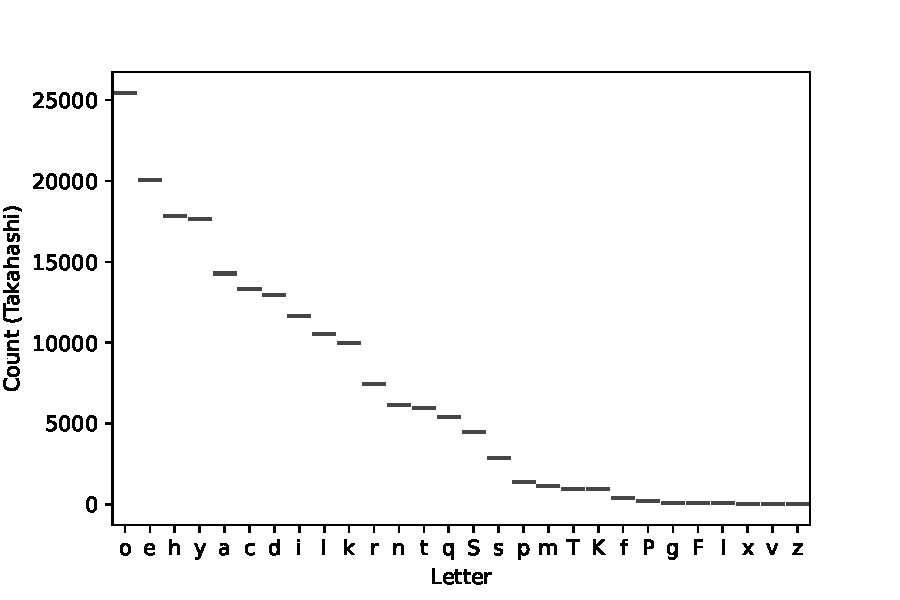
\includegraphics[scale=0.5]{figures/count_translit.pdf}
   \caption{Letter frequencies in Takahashi's transliteration.}
   \label{fig:count_translit}
\end{figure}

Determining what counts as \textit{one} glyph, though, is in some cases an interpretative act.
It seems straightforward to assume that {\eva c} and {\eva h} are one glyph (i.e., {\eva ch}).
Likewise, {\eva S} and {\eva h} could be interpreted as another glyph (i.e., {\eva Sh}).
Additionally, one \textit{might} interpret instances of {\eva cTh}, {\eva cKh}, {\eva cPh}, or {\eva cFh} as representing {\eva ch} (or {\eva Sh}), on the one hand, and {\eva t}, {\eva k}, {\eva p}, or {\eva f}, on the other.
Concerning those ``gallows'' characters, as they have come to be called, it is not clear whether {\eva t} and {\eva k} or {\eva p} and {\eva f} are variations of the same glyphs, only diverging in one small loop (as \cite{tiltman_voynich_1967} seems to have interpreted them).
In the following, the four gallows will be treated as distinct glyphs, as has become customary.
Accordingly, Table \ref{tab:count_c} gives frequencies for several {\eva c} combinations, taking into account four forms of ``pedestalled gallows'' (also see Figure \ref{fig:count_c}).
The table also includes three instances that bear some resemblance to Latin abbreviations (also see \cite[p. 95]{dimperio_voynich_1978}).

\begin{table}[ht]
\center
\begin{tabular}{ccrr}
   \hline
   Letter(s)      & Representation   & \multicolumn{2}{c}{Count}       \\
                  &                  & Takahashi   & Takahashi/Bauer   \\
   \hline\hline
   \texttt{ch}    & {\eva ch}        & 11,008      &                   \\
   \texttt{Sh}    & {\eva Sh}        &  4,501      &                   \\
   \texttt{cTh}   & {\eva cTh}       &    950      &                   \\
   \texttt{cKh}   & {\eva cKh}       &    906      &                   \\
   \texttt{cPh}   & {\eva cPh}       &    216      &                   \\
   \texttt{cFh}   & {\eva cFh}       &     74      &                   \\
   \texttt{c}     & {\eva c}         &    143      &                   \\
   \texttt{co}    & {\eva co}        &      9      &                   \\
   \texttt{cy}    & {\eva cy}        &      7      &                   \\
   \hline
                  &                  & 17,814      &                   \\
   \hline
\end{tabular}
\caption{Frequencies in Takahashi's transliteration for several {\eva c} combinations.}
\label{tab:count_c}
\end{table}

\begin{figure}
   \centering
   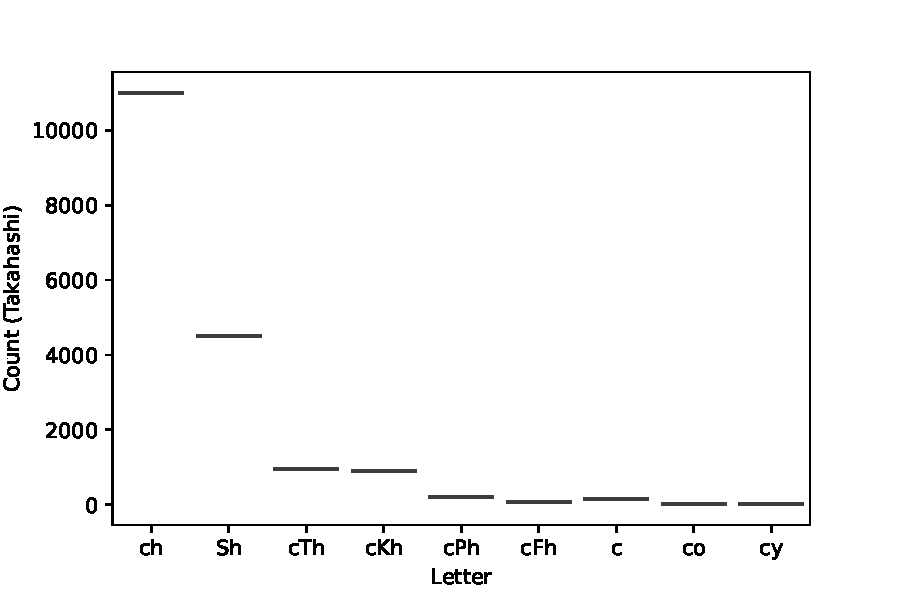
\includegraphics[scale=0.5]{figures/count_c.pdf}
   \caption{Frequencies in Takahashi's transliteration for several {\eva c} combinations.}
   \label{fig:count_c}
\end{figure}

Furthermore, while there are instances of a single {\eva i}, it is not clear whether instances like {\eva ii} and {\eva iii} or combinations with {\eva n} like {\eva in} or {\eva iin} represent separate glyphs.
Table \ref{tab:count_i} gives frequencies for several of those {\eva i} combinations (also see Figure \ref{fig:count_i}).
Assuming there are three glyphs {\eva i}, {\eva in}, and {\eva iin}, it is of course difficult to determine when there actually is a {\eva in} or a {\eva iin}.

\begin{table}[ht]
\center
\begin{tabular}{ccrr}
   \hline
   Letter(s)        & Representation   & \multicolumn{2}{c}{Count}       \\
                    &                  & Takahashi   & Takahashi/Bauer   \\
   \hline\hline
   \texttt{i}       & {\eva i}         &   590       &                   \\
   \texttt{ii}      & {\eva ii}        &   195       &                   \\
   \texttt{iii}     & {\eva iii}       &    10       &                   \\
   \texttt{n}       & {\eva n}         &   148       &                   \\
   \texttt{in}      & {\eva in}        & 1,752       &                   \\
   \texttt{iin}     & {\eva iin}       & 4,076       &                   \\
   \texttt{iiin}    & {\eva iiin}      &   154       &                   \\
   \texttt{iiiin}   & {\eva iiiin}     &     2       &                   \\
   \hline
                    &                  & 6,927       &                   \\
   \hline
\end{tabular}
\caption{Frequencies in Takahashi's transliteration for several {\eva i} combinations.}
\label{tab:count_i}
\end{table}

\begin{figure}
   \centering
   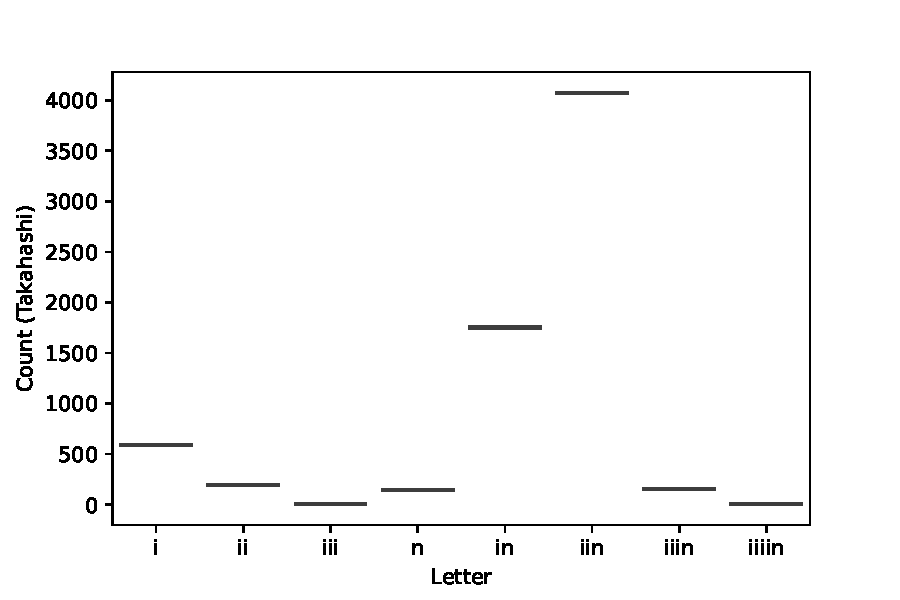
\includegraphics[scale=0.5]{figures/count_i.pdf}
   \caption{Frequencies in Takahashi's transliteration for several {\eva i} combinations.}
   \label{fig:count_i}
\end{figure}

This being said, I tentatively stipulate a set of 22 glyphs.
Table \ref{tab:count_glyph} gives frequencies for those glyphs (also see Figure \ref{fig:count_glyph}).
They are counted according to the following rules:

\begin{itemize}
   \item The glyphs {\eva a}, {\eva d}, {\eva e}, {\eva g}, {\eva I}, {\eva l}, {\eva m}, {\eva o}, {\eva q}, {\eva r}, {\eva s}, {\eva v}, {\eva x}, and {\eva y} are simply counted as before. Hence, frequencies are identical with Table \ref{tab:count_translit}.
   \item The glyph {\eva Sh} is counted every time {\eva S} and {\eva h} appear consecutively.
   \item The glyph {\eva ch} is counted every time {\eva c} and {\eva h} appear consecutively, as well as in cases where there is {\eva T}, {\eva K}, {\eva P}, or {\eva F} between them.
   \item The glyph {\eva t} is counted every time {\eva t} or {\eva T} appears.
   \item The glyph {\eva k} is counted every time {\eva k}, {\eva K}, or {\eva z} appears.
   \item The glyph {\eva p} is counted every time {\eva p} or {\eva P} appears.
   \item The glyph {\eva f} is counted every time {\eva f} or {\eva F} appears.
   \item The glyph {\eva in} is counted every time {\eva i} and {\eva n} appear consecutively without there being a preceding second {\eva i}.
   \item The glyph {\eva iin} is counted every time {\eva i}, {\eva i}, and {\eva n} appear consecutively.
   \item The glyph {\eva i} is counted every time it is not part of {\eva in} or {\eva iin} as well as in instances of {\eva I}.
\end{itemize}

\begin{table}[ht]
\center
\begin{tabular}{ccrrrr}
   \hline
   Letter(s)      & Glyph        & \multicolumn{4}{c}{Count (Percent)}                                     \\
                  &              & \multicolumn{2}{c}{Takahashi}   & \multicolumn{2}{c}{Takahashi/Bauer}   \\
   \hline\hline
   \texttt{o}     & {\eva o}     &  25,468   & (15.636)            &       &                               \\
   \texttt{e}     & {\eva e}     &  20,070   & (12.322)            &       &                               \\
   \texttt{y}     & {\eva y}     &  17,655   & (10.839)            &       &                               \\
   \texttt{a}     & {\eva a}     &  14,281   &  (8.768)            &       &                               \\
   \texttt{ch}    & {\eva ch}    &  13,154   &  (8.076)            &       &                               \\
   \texttt{d}     & {\eva d}     &  12,973   &  (7.965)            &       &                               \\
   \texttt{k}     & {\eva k}     &  10,934   &  (6.713)            &       &                               \\
   \texttt{l}     & {\eva l}     &  10,518   &  (6.458)            &       &                               \\
   \texttt{r}     & {\eva r}     &   7,456   &  (4.578)            &       &                               \\
   \texttt{t}     & {\eva t}     &   6,944   &  (4.263)            &       &                               \\
   \texttt{q}     & {\eva q}     &   5,423   &  (3.329)            &       &                               \\
   \texttt{Sh}    & {\eva Sh}    &   4,501   &  (2.763)            &       &                               \\
   \texttt{iin}   & {\eva iin}   &   4,232   &  (2.598)            &       &                               \\
   \texttt{s}     & {\eva s}     &   2,886   &  (1.772)            &       &                               \\
   \texttt{in}    & {\eva in}    &   1,752   &  (1.076)            &       &                               \\
   \texttt{p}     & {\eva p}     &   1,630   &  (1.001)            &       &                               \\
   \texttt{i}     & {\eva i}     &   1,240   &  (0.761)            &       &                               \\
   \texttt{m}     & {\eva m}     &   1,116   &  (0.685)            &       &                               \\
   \texttt{f}     & {\eva f}     &     505   &  (0.310)            &       &                               \\
   \texttt{g}     & {\eva g}     &      96   &  (0.059)            &       &                               \\
   \texttt{x}     & {\eva x}     &      35   &  (0.021)            &       &                               \\
   \texttt{v}     & {\eva v}     &       9   & (<0.001)            &       &                               \\
   \hline
                  &              & 162,878   &                     &       &                               \\
   \hline
\end{tabular}
\caption{Glyph frequencies in Takahashi's transliteration}
\label{tab:count_glyph}
\end{table}

\begin{figure}
   \centering
   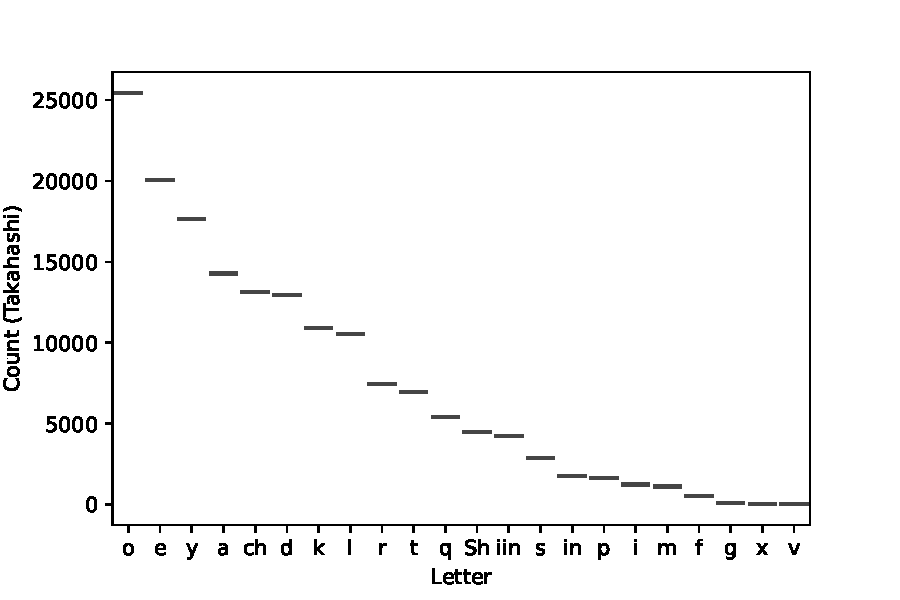
\includegraphics[scale=0.5]{figures/count_glyph.pdf}
   \caption{Glyph frequencies in Takahashi's transliteration.}
   \label{fig:count_glyph}
\end{figure}

\subsubsection{Glyph and Word Frequencies for Currier Languages}\label{sec:frequencies_currier}

\subsubsection{Glyph and Word Frequencies for Hands}\label{sec:frequencies_hands}


%%%%%%%%%%%
% ENTROPY %
%%%%%%%%%%%
\subsection{Entropy}\label{sec:entropy}
Next, let's take a look at the manuscript's entropy.
To this end, I utilize the conceptualization of information entropy by \citet{shannon_mathematical_1948}, basically measuring the variability of glyphs in the manuscript.
Entropy $H$ can be defined as shown in (\ref{eq:shannon}), where $p_{z}$ denotes the probability of $z$, with $z$ being an element of the alphabet $Z$.

\begin{equation}\label{eq:shannon}
   H=-\sum_{z\in Z}p_{z}\log_{2}p_{z}
\end{equation}

\noindent To calculate the entropy, I suppose the above stipulated glyphs to form alphabet $Z$ (see Table \ref{tab:count_glyph}).
Accordingly, changes to the corpus are made so that each stipulated glyph has a single corresponding character in the transliteration.
Changes are made according to the following rules:

\begin{itemize}
   \item The glyph {\eva Sh} is represented by \texttt{Sh} in EVA. For calculating the entropy, every time \texttt{S} and \texttt{h} appear consecutively, they are replaced by \texttt{1}
   \item The glyph {\eva ch} is represented by \texttt{ch} in EVA. Every time \texttt{c} and \texttt{h} appear consecutively, they are replaced by \texttt{2}. Following the above stated rules for glyph counting, {\eva ch} is also believed to be present when {\eva c} and {\eva h} are separated by {\eva T}, {\eva K}, {\eva P}, or {\eva F}, represented by \texttt{T}, \texttt{K}, \texttt{P}, or \texttt{F} in EVA. In those cases, it is believed that {\eva t}, {\eva k}, {\eva p}, or {\eva f} are also present. They are represented by \texttt{t}, \texttt{k}, \texttt{p}, or \texttt{f}  in EVA. Hence, they are replaced by \texttt{2t}, \texttt{2k}, \texttt{2p}, or \texttt{2f}.
   \item The glyph {\eva z}, represented by \texttt{z} in EVA, is counted as {\eva k}, represented by \texttt{k} in EVA. Hence, every \texttt{z} is replaced by \texttt{k}.
   \item The glyph {\eva iin} is represented by \texttt{iin} in EVA. Every time \texttt{i}, \texttt{i}, and \texttt{n} appear consecutively, they are replaced by \texttt{3}.   
   \item The glyph {\eva in} is represented by \texttt{in} in EVA. Every time \texttt{i} and \texttt{n} appear consecutively, they are replaced by \texttt{4}.
   \item Lastly, the glyph {\eva I}, represented by \texttt{I} in EVA, is counted as {\eva i}, represented by \texttt{i} in EVA. Hence, every \texttt{I} is replaced by \texttt{i}.
\end{itemize}

\noindent Calculating the entropy for this converted corpus results in $H=3.866$.
As comparisons, Table \ref{tab:entropy} also offers the entropy values for the unconverted transliteration as well as for a randomly generated text consisting of 22 different characters and being 234,956 characters long (just as the converted transliteration).

\begin{table}[ht]
\center
\begin{tabular}{lr}
   \hline
   Corpus                        & \multicolumn{1}{c}{$H$}   \\
   \hline\hline
   Takahashi                     & 4.021                     \\
   Takahashi (converted)         & 3.866                     \\
   Takahashi/Bauer               &                           \\
   Takahashi/Bauer (converted)   &                           \\
   Random text                   & 4.459                     \\
   \hline
\end{tabular}
\caption{Entropy ($H$) for different transliterations.}
\label{tab:entropy}
\end{table}


%%%%%%%%%%%%%%
% REFERENCES %
%%%%%%%%%%%%%%
\clearpage
\printbibliography


\end{document}
